\chapter{Zoekmethodes}
\label{s:searchMethods}
\chapterquote{Toen ik moe was van zoeken, leerde ik vinden.}{Friedrich Nietzsche, Duits dichter en filosoof (1844-1900)}
Indien we een state-space gebouwd hebben, kunnen we vervolgens een algoritme ontwikkelen die door deze state-space zoekt naar een oplossing. Hiervoor bestaan er verschillende methodes die kunnen gebruikt worden: De \termenglos{basic search methods}{Een set van zoekalgoritmen die we kunnen gebruiken om een oplossing te zoeken in een state-space.}.
\paragraph{Evaluatie-criteria}
We kunnen een zoekmethode evalueren op volgende criteria:
\begin{itemize}
 \item \termenglos{Completeness}{Een eigenschap van een zoek algoritme. Indien een zoekalgoritme compleet is, vindt het altijd de oplossing indien er een oplossing voor het probleem bestaat.}: vindt het algoritme altijd een oplossing (indien er een oplossing bestaat)
 \item \termenglos{Speed}{Een eigenschap van een zoek algoritme. De snelheid is de worst-case tijdscomplexiteit van het zoekalgoritme.}: de worst-case tijdscomplexiteit
 \item \termenglos{Memory}{Een eigenschap van een zoek algoritme. De snelheid is de worst-case geheugencomplexiteit van het zoekalgoritme.}: de worst-case geheugencomplexiteit
 \item \termenglos{Optimaliteit}{Een eigenschap van een zoekalgoritme. Indien een zoekalgoritme optimaal is, vindt het altijd de optimale oplossing (optimaal volgens een zelfgekozen metriek).}: zoeken we de optimale oplossing, of is \'e\'en oplossing voldoende
\end{itemize}
Voor complexiteitsanalyses zullen we gebruikmaken van onderstaande parameters:
\begin{itemize}
 \item $d$: de diepte van de boom
 \item $b$: de vertakkingsfactor
 \item $m$: de diepte van de minst diepe oplossing
 \item $\delta$: de kleinste kost tussen twee staten (zie \ref{ss:optimalSearch})
\end{itemize}
\section{Leidend Voorbeeld: Wegenplan}
\begin{leftbar}
Doorheen deze sectie zullen we vaak concepten verduidelijken met behulp van een voorbeeld. Dit voorbeeld wordt hieronder kort toegelicht. Het betreft een sterk vereenvoudigd wegenplan. Hierbij willen we vanuit $S$ (de begintoestand), $G$ (het doel) bereiken. We gaan er vanuit dat er slechts 9 steden bestaan: $A$ (Antwerpen), $B$ (Brussel), $C$ (Charleroi), $D$ (Durbuy), $E$ (Eeklo), $F$ (Fosses-la-Ville), $G$ (Geel), $H$ (Hoei) en $S$ (Sint-Niklaas). Verder bestaan er alleen wegen die tussen twee steden lopen met een bepaalde afstand in kilometer. Dit wordt weergegeven op figuur \ref{fig:searchMapCity}.
\end{leftbar}
\begin{figure}[htb]
\centering
\begin{tikzpicture}[scale=0.7,city/.style={shape=circle,draw=black},dist/.style={halfway,sloped,below},heur/.style={gray,anchor=south}]
\def\sqrttf{4.898979486};
\def\sqrts{2.449489743};
\def\xs{-24*\sqrts/25-16/25};
\def\ys{32*\sqrts/25-12/25};
\def\xg{8.71151};%24*\sqrts/25+53/25
\def\yg{1.28363};%18*\sqrts/25-12/25
\def\xh{3.90957};
\def\yh{-2.31377};
\node[city] (S) at (\xs,\ys) {$S$};
\node[city] (A) at (-1,\sqrttf) {$A$};
\node[city] (B) at (3,\sqrttf) {$B$};
\node[city] (C) at (7,\sqrttf) {$C$};
\node[city] (D) at (0,0) {$D$};
\node[city] (E) at (2,0) {$E$};
\node[city] (F) at (6,0) {$F$};
\node[city] (G) at (\xg,\yg) {$G$};
\node[city] (H) at (\xh,\yh) {$H$};
\node[heur] (Sh) at (S.north) {$11.8$};
\node[heur] (Ah) at (A.north) {$10.4$};
\node[heur] (Bh) at (B.north) {$6.8$};
\node[heur] (Ch) at (C.north) {$4$};
\node[heur] (Dh) at (D.north) {$8.8$};
\node[heur] (Eh) at (E.north) {$6.8$};
\node[heur] (Fh) at (F.north) {$3$};
\node[heur] (Gh) at (G.north) {$0$};
\node[heur] (Hh) at (H.north) {$6$};
\draw (S) to node[dist]{3} (A) to node[dist]{5} (D) to node[dist]{2} (E) to node[dist]{5} (B) to node[dist]{4} (C);
\draw (E) to node[dist]{4} (F) to node[dist,above]{3} (G);
\draw (E) to node[dist]{3} (H) to node[dist]{6} (G);
\draw (S) to node[dist]{4} (D);
\draw (A) to node[dist]{4} (B);
\end{tikzpicture}
\caption{Voorstelling van een door ons beschouwd wegenplan}
\label{fig:searchMapCity}
\end{figure}
\begin{leftbar}
Als overgangsregels beschouwen we iedere weg naar iedere stad die we tot dan toe nog niet bezocht hebben. Vanuit $S$ kunnen we dus naar twee andere toestanden: $A$ en $D$. Indien we vervolgens verder de productieregels op deze toestanden toepassen, bekomen we een boom zoals op figuur \ref{fig:searchTreeCity}.
\end{leftbar}
\begin{figure}[htb]
\centering
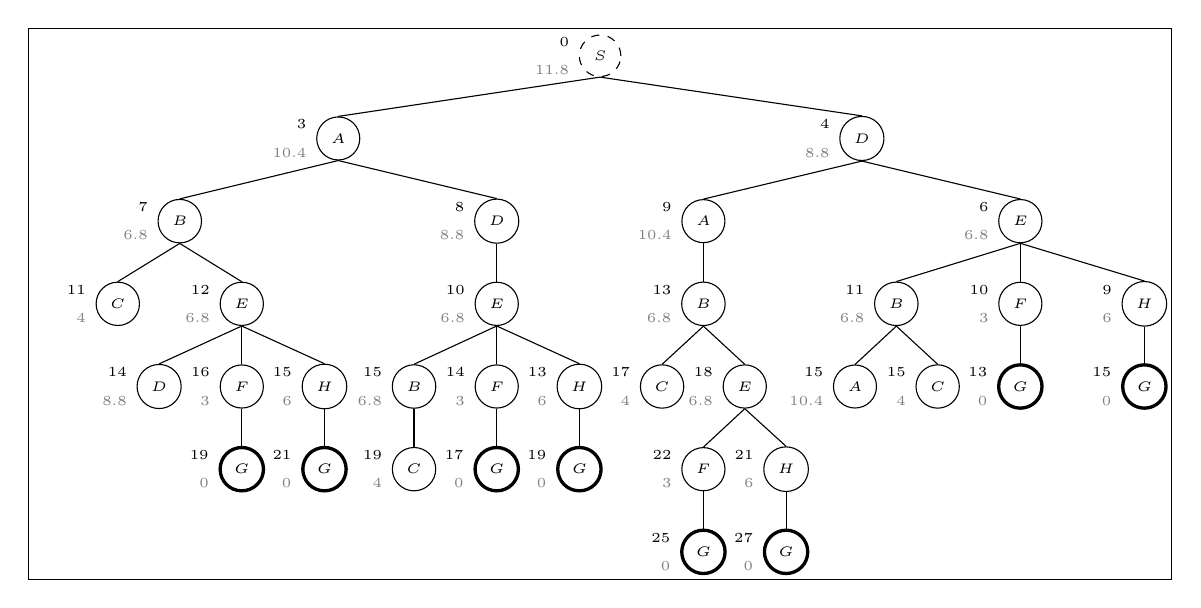
\begin{tikzpicture}[scale=1.4,city/.style={shape=circle,draw=black},costc/.style={anchor=south east},heurh/.style={anchor=north east,gray},cityG/.style={city,very thick},cityM/.style={city,fill=gray}]
\def\dy{-0.75};
\def\dxa{4.75};
\def\dxb{2.875};
\def\dxc{1.125};
\def\dxd{0.75};
\def\dxe{0.75};

\draw (-0.5*\dxa-0.5*\dxb-\dxc-0.25,0.25) rectangle (0.5*\dxa+0.5*\dxb+\dxc+0.25,6*\dy-0.25);

\node[city,dashed] (S) at (0,0) {\tiny $S$};
\node[costc] (Sc) at (S.west) {\tiny 0};
\node[heurh] (Sh) at (S.west) {\tiny 11.8};

\node[city] (A) at (-0.5*\dxa,\dy) {\tiny $A$};
\node[costc] (Ac) at (A.west) {\tiny 3};
\node[heurh] (Ah) at (A.west) {\tiny 10.4};
\draw (S.south) -- (A.north);
\node[city] (D) at (0.5*\dxa,\dy) {\tiny $D$};
\node[costc] (Dc) at (D.west) {\tiny 4};
\node[heurh] (Dh) at (D.west) {\tiny 8.8};
\draw (S.south) -- (D.north);

\node[city] (B) at (-0.5*\dxa-0.5*\dxb,2*\dy) {\tiny $B$};
\node[costc] (Bc) at (B.west) {\tiny 7};
\node[heurh] (Bh) at (B.west) {\tiny 6.8};
\draw (A.south) -- (B.north);
\node[city] (D2) at (-0.5*\dxa+0.5*\dxb,2*\dy) {\tiny $D$};
\node[costc] (D2c) at (D2.west) {\tiny 8};
\node[heurh] (D2h) at (D2.west) {\tiny 8.8};
\draw (A.south) -- (D2.north);
\node[city] (A2) at (0.5*\dxa-0.5*\dxb,2*\dy) {\tiny $A$};
\node[costc] (A2c) at (A2.west) {\tiny 9};
\node[heurh] (A2h) at (A2.west) {\tiny 10.4};
\draw (D.south) -- (A2.north);
\node[city] (E) at (0.5*\dxa+0.5*\dxb,2*\dy) {\tiny $E$};
\node[costc] (Ec) at (E.west) {\tiny 6};
\node[heurh] (Eh) at (E.west) {\tiny 6.8};
\draw (D.south) -- (E.north);

\node[city] (C) at (-0.5*\dxa-0.5*\dxb-0.5*\dxc,3*\dy) {\tiny $C$};
\node[costc] (Cc) at (C.west) {\tiny 11};
\node[heurh] (Ch) at (C.west) {\tiny 4};
\draw (B.south) -- (C.north);
\node[city] (E2) at (-0.5*\dxa-0.5*\dxb+0.5*\dxc,3*\dy) {\tiny $E$};
\node[costc] (E2c) at (E2.west) {\tiny 12};
\node[heurh] (E2h) at (E2.west) {\tiny 6.8};
\draw (B.south) -- (E2.north);
\node[city] (E3) at (-0.5*\dxa+0.5*\dxb,3*\dy) {\tiny $E$};
\node[costc] (E3c) at (E3.west) {\tiny 10};
\node[heurh] (E3h) at (E3.west) {\tiny 6.8};
\draw (D2.south) -- (E3.north);
\node[city] (B2) at (0.5*\dxa-0.5*\dxb,3*\dy) {\tiny $B$};
\node[costc] (B2c) at (B2.west) {\tiny 13};
\node[heurh] (B2h) at (B2.west) {\tiny 6.8};
\draw (A2.south) -- (B2.north);
\node[city] (B3) at (0.5*\dxa+0.5*\dxb-\dxc,3*\dy) {\tiny $B$};
\node[costc] (B3c) at (B3.west) {\tiny 11};
\node[heurh] (B3h) at (B3.west) {\tiny 6.8};
\draw (E.south) -- (B3.north);
\node[city] (F) at (0.5*\dxa+0.5*\dxb,3*\dy) {\tiny $F$};
\node[costc] (Fc) at (F.west) {\tiny 10};
\node[heurh] (Fh) at (F.west) {\tiny 3};
\draw (E.south) -- (F.north);
\node[city] (H) at (0.5*\dxa+0.5*\dxb+\dxc,3*\dy) {\tiny $H$};
\node[costc] (Hc) at (H.west) {\tiny 9};
\node[heurh] (Hh) at (H.west) {\tiny 6};
\draw (E.south) -- (H.north);

\node[city] (D3) at (-0.5*\dxa-0.5*\dxb+0.5*\dxc-\dxd,4*\dy) {\tiny $D$};
\node[costc] (D3c) at (D3.west) {\tiny 14};
\node[heurh] (D3h) at (D3.west) {\tiny 8.8};
\draw (E2.south) -- (D3.north);
\node[city] (F2) at (-0.5*\dxa-0.5*\dxb+0.5*\dxc,4*\dy) {\tiny $F$};
\node[costc] (F2c) at (F2.west) {\tiny 16};
\node[heurh] (F2h) at (F2.west) {\tiny 3};
\draw (E2.south) -- (F2.north);
\node[city] (H2) at (-0.5*\dxa-0.5*\dxb+0.5*\dxc+\dxd,4*\dy) {\tiny $H$};
\node[costc] (H2c) at (H2.west) {\tiny 15};
\node[heurh] (H2h) at (H2.west) {\tiny 6};
\draw (E2.south) -- (H2.north);
\node[city] (B4) at (-0.5*\dxa+0.5*\dxb-\dxd,4*\dy) {\tiny $B$};
\node[costc] (B4c) at (B4.west) {\tiny 15};
\node[heurh] (B4h) at (B4.west) {\tiny 6.8};
\draw (E3.south) -- (B4.north);
\node[city] (F3) at (-0.5*\dxa+0.5*\dxb,4*\dy) {\tiny $F$};
\node[costc] (F3c) at (F3.west) {\tiny 14};
\node[heurh] (F3h) at (F3.west) {\tiny 3};
\draw (E3.south) -- (F3.north);
\node[city] (H3) at (-0.5*\dxa+0.5*\dxb+\dxd,4*\dy) {\tiny $H$};
\node[costc] (H3c) at (H3.west) {\tiny 13};
\node[heurh] (H3h) at (H3.west) {\tiny 6};
\draw (E3.south) -- (H3.north);
\node[city] (C2) at (0.5*\dxa-0.5*\dxb-0.5*\dxd,4*\dy) {\tiny $C$};
\node[costc] (C2c) at (C2.west) {\tiny 17};
\node[heurh] (C2h) at (C2.west) {\tiny 4};
\draw (B2.south) -- (C2.north);
\node[city] (E4) at (0.5*\dxa-0.5*\dxb+0.5*\dxd,4*\dy) {\tiny $E$};
\node[costc] (E4c) at (E4.west) {\tiny 18};
\node[heurh] (E4h) at (E4.west) {\tiny 6.8};
\draw (B2.south) -- (E4.north);
\node[city] (A3) at (0.5*\dxa+0.5*\dxb-\dxc-0.5*\dxd,4*\dy) {\tiny $A$};
\node[costc] (A3c) at (A3.west) {\tiny 15};
\node[heurh] (A3h) at (A3.west) {\tiny 10.4};
\draw (B3.south) -- (A3.north);
\node[city] (C3) at (0.5*\dxa+0.5*\dxb-\dxc+0.5*\dxd,4*\dy) {\tiny $C$};
\node[costc] (C3c) at (C3.west) {\tiny 15};
\node[heurh] (C3h) at (C3.west) {\tiny 4};
\draw (B3.south) -- (C3.north);
\node[cityG] (G) at (0.5*\dxa+0.5*\dxb,4*\dy) {\tiny $G$};
\node[costc] (Gc) at (G.west) {\tiny 13};
\node[heurh] (Gh) at (G.west) {\tiny 0};
\draw (F.south) -- (G.north);
\node[cityG] (G2) at (0.5*\dxa+0.5*\dxb+\dxc,4*\dy) {\tiny $G$};
\node[costc] (G2c) at (G2.west) {\tiny 15};
\node[heurh] (G2h) at (G2.west) {\tiny 0};
\draw (H.south) -- (G2.north);

\node[cityG] (G3) at (-0.5*\dxa-0.5*\dxb+0.5*\dxc,5*\dy) {\tiny $G$};
\node[costc] (G3c) at (G3.west) {\tiny 19};
\node[heurh] (G3h) at (G3.west) {\tiny 0};
\draw (F2.south) -- (G3.north);
\node[cityG] (G4) at (-0.5*\dxa-0.5*\dxb+0.5*\dxc+\dxd,5*\dy) {\tiny $G$};
\node[costc] (G4c) at (G4.west) {\tiny 21};
\node[heurh] (G4h) at (G4.west) {\tiny 0};
\draw (H2.south) -- (G4.north);
\node[city] (C4) at (-0.5*\dxa+0.5*\dxb-\dxd,5*\dy) {\tiny $C$};
\node[costc] (C4c) at (C4.west) {\tiny 19};
\node[heurh] (C4h) at (C4.west) {\tiny 4};
\draw (B4.south) -- (C4.north);
\node[cityG] (G5) at (-0.5*\dxa+0.5*\dxb,5*\dy) {\tiny $G$};
\node[costc] (G5c) at (G5.west) {\tiny 17};
\node[heurh] (G5h) at (G5.west) {\tiny 0};
\draw (F3.south) -- (G5.north);
\node[cityG] (G6) at (-0.5*\dxa+0.5*\dxb+\dxd,5*\dy) {\tiny $G$};
\node[costc] (G6c) at (G6.west) {\tiny 19};
\node[heurh] (G6h) at (G6.west) {\tiny 0};
\draw (H3.south) -- (G6.north);
\node[city] (F4) at (0.5*\dxa-0.5*\dxb+0.5*\dxd-0.5*\dxe,5*\dy) {\tiny $F$};
\node[costc] (F4c) at (F4.west) {\tiny 22};
\node[heurh] (F4h) at (F4.west) {\tiny 3};
\draw (E4.south) -- (F4.north);
\node[city] (H4) at (0.5*\dxa-0.5*\dxb+0.5*\dxd+0.5*\dxe,5*\dy) {\tiny $H$};
\node[costc] (H4c) at (H4.west) {\tiny 21};
\node[heurh] (H4h) at (H4.west) {\tiny 6};
\draw (E4.south) -- (H4.north);

\node[cityG] (G7) at (0.5*\dxa-0.5*\dxb+0.5*\dxd-0.5*\dxe,6*\dy) {\tiny $G$};
\node[costc] (G7c) at (G7.west) {\tiny 25};
\node[heurh] (G7h) at (G7.west) {\tiny 0};
\draw (F4.south) -- (G7.north);
\node[cityG] (G8) at (0.5*\dxa-0.5*\dxb+0.5*\dxd+0.5*\dxe,6*\dy) {\tiny $G$};
\node[costc] (G8c) at (G8.west) {\tiny 27};
\node[heurh] (G8h) at (G8.west) {\tiny 0};
\draw (H4.south) -- (G8.north);
\end{tikzpicture}
\caption{Zoekboom van het wegenplan}
\label{fig:searchTreeCity}
\end{figure}
\begin{leftbar}
Als heuristiek (zie \ref{sss:heuristicFunction}) nemen we tot slot de afstand in vogelvlucht tussen de stad in kwestie, en $G$ zelf. Deze wordt in het grijs op het wegenplan aangegeven. We zullen in deze sectie heel wat zoekalgoritmen uitvoeren op deze boom, om zo de concrete werking te verduidelijken. Deze afbeeldingen staan niet in de tekst zelf, maar staan in \ref{ss:cityFigures} op pagina \pageref{ss:cityFigures}.
\end{leftbar}
\section{Blind Search Methods}
Indien we geen specifieke kennis over het probleem hebben, of deze te complex/lastig is om te formuleren kunnen we een \termenglos{Blind Search Method}{Een subset van de basic search methods waarbij we geen specifieke kennis over het probleem hebben.} gebruiken. Het is evident dat zoeken zonder probleemgerelateerde informatie ineffici\"ent is. Bij deze methodes zijn we ook niet ge\"interesseerd in de optimale oplossing.
\subsection{Depth-First Search}
Bij \termenglos{Depth-First Search}{Een blind search algoritme die blijft productieregels op een toestand toepassen totdat we het doel gevonden hebben, of geen productieregels meer toe te passen zijn. In het laatste geval voeren we backtracking uit tot we terug bij een toestand zijn waar we een alternatieve productieregel kunnen volgen.} of \termen{Diepte-eerst zoeken} volgen we een bepaalde productieregel vanaf de begintoestand. Vervolgens blijven we deze regel recursief toepassen tot we vast zitten. Indien we een doel gevonden hebben is het algoritme ten einde. Indien het niet het doel is, zal het algoritme de laatste productieregel ongedaan maken en een andere in de plaats stellen. Indien er geen ongebruikte regels meer voor handen zijn maken we de regels daarvoor ongedaan tot we terug een regel kunnen kiezen. Een andere naam hiervoor is \termenglos{Chronological Backtracking}{Een backtrackingsmechanisme waarbij we  de laatst gekozen productieregels ongedaan maken totdat we een toestand tegenkomen waarbij we een nog niet onderzocht alternatief tegenkomen.}. Deze zoekmethode wordt ge\"illustreerd in \algref{alg:depthFirst}. We voorkomen dat we in een lus terechtkomen (indien de productieregel dit toelaten) door telkens we een toestand genereren te controleren of \'e\'en van zijn voorouders identiek aan die toestand is. Indien dit zo is, zullen we die toestand niet meer verder evalueren. Dit systeem noemen we \termenglos{Loopdetectie}{Een detectiemechanisme die detecteert dat we door een sequentie van productieregels, in een reeds bezochte toestand tegenkomen. In dat geval dienen we backtracking toe te passen.}.
\begin{algorithm}[htb]                      % enter the algorithm environment
\caption{Depth-First zoekalgoritme}          % give the algorithm a caption
\label{alg:depthFirst}                           % and a label for \ref{} commands later in the document
\begin{algorithmic}[1]                    % enter the algorithmic environment
\STATE $\queue\leftarrow\mbox{Path containing the root}$
\WHILE{$\notempty{\queue}\wedge\neg\goalreached{\queue}$}
\STATE $r\leftarrow\dequeue{\queue}$
\STATE $R\leftarrow\createnewpaths{r}$
\STATE $\removeloops{R}$
\STATE $\enqueuefront{\queue,R}$
\ENDWHILE
\IF{$\goalreached{\queue}$}
\RETURN $\success$
\ELSE
\RETURN $\failure$
\ENDIF
\end{algorithmic}
\end{algorithm}
\paragraph{Complexiteiten}
We zullen nu de tijd- en geheugencomplexiteit voor Depth-First analyseren. Hierbij zullen we systemen zoals het loopdetectie systeem buiten beschouwing laten. We gaan er dus vanuit dat we een pad analyseren in \bigoh{1}. Dit is uiteraard niet het geval, en zal in andere algoritmes zelfs oplopen tot lange procedures. We zijn dus meer ge\"interesseerd in het aantal maal we de while-lus uitvoeren, en beschouwen dit als tijdscomplexiteit. 
\paragraph{}
Indien we dit toepassen op Depth-First stellen we vast dat we een tijdscomplexiteit van \bigoh{b^d} uitkomen. Vrij vertaald betekent dit dus dat we de volledige boom doorlopen. Dit is te beargumenteren: stel dat de oplossing zich in de meest rechtse tak bevindt. In dat geval, zal Depth-First eerst alle andere paden van links naar rechts doorlopen. Het maakt niet zoveel uit op welke diepte de oplossing zich bevindt (indien niet onmiddellijk onder de wortel). Deze eigenschap kan ook de compleetheid van het algoritme ook in gevaar brengen. Indien we met een oneindig diepe boom te maken hebben. Waarbij we telkens verder op een bepaalde knoop kunnen produceren, zal het algoritme nooit stoppen. We moeten dus over productieregels beschikken die vroeg of laat ieder pad doen stoppen, om dit algoritme volledig te doen werken.
\paragraph{}
Het geheugengebruik van Depth-First is beter. Op ieder niveau is op ieder moment hooguit \'e\'en knoop ge\"expandeert, bijgevolg zitten er in de $\queue$ hooguit \bigoh{b\cdot d} knopen. Namelijk per diepte $b$ verschillende knopen.	
\paragraph{}
Indien we dit samenvatten bekomen we volgende criteria:
\begin{center}
\begin{tabular}{ll}
\textbf{Compleet}:&Ja, indien geen oneindig diepe boom\\
\textbf{Snelheid}:&\bigoh{b^d}\\
\textbf{Geheugen}:&\bigoh{b\cdot d}\\
\textbf{Optimaal}:&Nee
\end{tabular}
\end{center}
\begin{leftbar}
We illustreren de werking van dit algoritme op het wegenplan in figuur \ref{fig:depthFirstCity} op pagina \pageref{fig:depthFirstCity}.
\end{leftbar}
\subsection{Breadth-First Search}
Bij \termen{Breadth-First Search}{Een blind search algoritme waarbij we gelaagd werken: we houden een lijst bij van alle toestanden (samen met het pad die tot deze toestanden leidde) die we na $i$ productieregels op de begintoestanden kunnen bereiken. Vervolg expanderen we \'e\'en van deze toestanden en voegen de toestanden van de volgende laag achteraan in de wachtrij toe.} of de \termen{Breedte-eerst zoeken} zoekmethode wordt een laag aan oplossingen afgewerkt alvorens er een nieuwe laag wordt bekeken. Concreet betekent dit dus dat de kinderen van een ge\"evalueerde knoop achteraan in een wachtrij geplaatst worden, en dus pas behandeld worden wanneer alle andere knopen van dezelfde boom toegevoegd zijn. Dit wordt ge\"illustreerd in \algref{alg:breadthFirst}.
\begin{algorithm}[htb]                      % enter the algorithm environment
\caption{Breadth-First zoekalgoritme}          % give the algorithm a caption
\label{alg:breadthFirst}                           % and a label for \ref{} commands later in the document
\begin{algorithmic}[1]                    % enter the algorithmic environment
\STATE $\queue\leftarrow\mbox{Path containing the root}$
\WHILE{$\notempty{\queue}\wedge\neg\goalreached{\queue}$}
\STATE $r\leftarrow\dequeue{\queue}$
\STATE $R\leftarrow\createnewpaths{r}$
\STATE $\removeloops{R}$
\STATE $\enqueueback{\queue,R}$
\ENDWHILE
\IF{$\goalreached{\queue}$}
\RETURN $\success$
\ELSE
\RETURN $\failure$
\ENDIF
\end{algorithmic}
\end{algorithm}
\paragraph{Complexiteiten}
In tijdscomplexiteit is een breedte eerst benadering in de meeste gevallen beter. Het algoritme zal immers alleen de boom expanderen tot de diepte waar een doel zich bevindt. De boom die we bekomen tot een diepte $m$ telt \bigoh{b^m} knopen. Bijgevolg hebben we dus ook \bigoh{b^{m-1}} evaluaties gedaan. Of eenvoudiger \bigoh{b^m}. Een ander voordeel van een Breedte-Eerst benadering is dat ook oneindig diepe bomen ge\"evalueerd kunnen worden. Bovendien zal het algoritme als oplossing een pad teruggeven met het minimale aantal stappen om tot een oplossing te komen (niet te verwarren met goedkoopste bij optimaal zoeken, het is niet omdat we het minste aantal steden passeren, dat we ook het minste kilometers afleggen).
\paragraph{}
De ommezijde van deze medaille is dat het geheugen erg ineffici\"ent gebruikt wordt. Dit moet immers telkens alle paden bijhouden op een diepte $m$. Dit is uiteraard eveneens gelijk aan \bigoh{b^m}. Omdat bij een hoge $m$ of $b$ het geheugengebruik makkelijk grote proporties aanneemt waarbij zelf moderne geheugens soms moeten afhaken is Breedte-Eerst alleen geschikt voor kleine problemen.
\paragraph{}
Samenvattend bekomen we dus volgende criteria:
\begin{center}
\begin{tabular}{ll}
\textbf{Compleet}:&Ja, zelfs de kortste\\
\textbf{Snelheid}:&\bigoh{b^m}\\
\textbf{Geheugen}:&\bigoh{b^m}\\
\textbf{Optimaal}:&Nee, wel het kortst
\end{tabular}
\end{center}
\begin{leftbar}
We illustreren de werking van dit algoritme op het wegenplan in figuur \ref{fig:breadthFirstCity} op pagina \pageref{fig:breadthFirstCity}.
\end{leftbar}
\subsection{Non-Deterministic Search}
Bij \termen{Non-Deterministic Search}{Een blind search algoritme waarbij we in willekeurige volgorde een toestand nemen, de toestanden na het toepassen van een productieregel genereren en deze toevoegen in de wachtrij.} of de \termen{Niet-deterministisch zoeken} zoekmethode worden de gegenereerde kinderen op toevallige plaatsen in de wachtrij gezet. Het gevolg is dus dat de we toevallig de boom expanderen. Soms kunnen deze methodes tot snelle resultaten leiden, anderzijds is de tijdsduur niet te berekenen. Dit wordt ge\"illustreerd in \algref{alg:nonDeterministic}.
\begin{algorithm}[htb]                      % enter the algorithm environment
\caption{Non-Deterministic zoekalgoritme}          % give the algorithm a caption
\label{alg:nonDeterministic}                           % and a label for \ref{} commands later in the document
\begin{algorithmic}[1]                    % enter the algorithmic environment
\STATE $\queue\leftarrow\mbox{Path containing the root}$
\WHILE{$\notempty{\queue}\wedge\neg\goalreached{\queue}$}
\STATE $r\leftarrow\dequeue{\queue}$
\STATE $R\leftarrow\createnewpaths{r}$
\STATE $\removeloops{R}$
\STATE $\enqueuerandom{\queue,R}$
\ENDWHILE
\IF{$\goalreached{\queue}$}
\RETURN $\success$
\ELSE
\RETURN $\failure$
\ENDIF
\end{algorithmic}
\end{algorithm}
\paragraph{Complexiteiten}
Het berekenen van de complexiteiten is behoorlijk eenvoudig: we weten eenvoudigweg niet hoe de knopen ge\"evalueerd zullen worden. In het slechtste geval wordt telkens een foute knoop gekozen, en moeten we dus eerst de volledige boom evalueren. De tijdscomplexiteit is dus \bigoh{b^d}. Dit algoritme zal echter niet vastlopen op oneindig diepe bomen. Vroeg of laat zal het de juiste combinatie van knopen evalueren om tot een oplossing te komen. Hoe lang dit duurt is echter onmogelijk te voorspellen. Verder kunnen we ook eerst alle knopen evalueren zodat we de onderste laag van onze boom in het geheugen opslaan. De geheugencomplexiteit is dus ook gelijk aan \bigoh{b^d}.
\paragraph{}
Indien we dus het loopdetectie-systeem even buiten beschouwing laten in onze tijds- en geheugencomplexiteitsanalyse bekomen we volgende criteria:
\begin{center}
\begin{tabular}{ll}
\textbf{Compleet}:&Ja\\
\textbf{Snelheid}:&\bigoh{b^d}\\
\textbf{Geheugen}:&\bigoh{b^d}\\
\textbf{Optimaal}:&Nee
\end{tabular}
\end{center}
\begin{leftbar}
 Een mogelijk scenario van dit algoritme is weergegeven in figuur \ref{fig:nonDeterministicCity} op pagina \pageref{fig:nonDeterministicCity}.
\end{leftbar}
\subsection{Iterative Deepening Search}
Een in het algemeen interessante zoekmethode is \termen{Iterative Deepening Search} of \termen{Iteratief verdiepend zoeken}. Deze methode maakt gebruik van het \termen{Depth-limited search} algoritme, dit is een algoritme die een implementatie is van Depth First, maar waarbij vanaf een bepaalde diepte gestopt wordt. Iterative Deepening Search maakt van deze methode gebruik door de diepte-limiet parameter op een bepaalde beginwaarde te zetten, en deze telkens te verhogen zolang er niets gevonden wordt. Dit wordt ge\"illustreerd in \algref{alg:iterativeDeepening}.
\begin{algorithm}[htb]                      % enter the algorithm environment
\caption{Iterative Deepening zoekalgoritme}          % give the algorithm a caption
\label{alg:iterativeDeepening}                           % and a label for \ref{} commands later in the document
\begin{algorithmic}[1]                    % enter the algorithmic environment
\STATE $\queue\leftarrow\varnothing$
\STATE $\depth\leftarrow1$\COMMENT{Or any other offset depth}
\WHILE{$\neg\goalreached{\queue}$}
\STATE\COMMENT{Start Depth-Limited Search}
\STATE $\queue\leftarrow\mbox{Path containing the root}$
\WHILE{$\notempty{\queue}\wedge\neg\goalreached{\queue}$}
\STATE $r\leftarrow\dequeue{\queue}$
\IF{$\depthNode{r}<\depth$}
\STATE $R\leftarrow\createnewpaths{r}$
\STATE $\removeloops{R}$
\STATE $\enqueuefront{\queue,R}$
\ENDIF
\ENDWHILE
\STATE\COMMENT{End Depth-Limited Search}
\STATE $\depth\leftarrow\depth+1$
\ENDWHILE
\end{algorithmic}
\end{algorithm}
\paragraph{Complexiteiten}
De complexiteit van Iterative Deepening berekenen we als volgt. We genereren een iteratie op Depth-First, hierbij zullen we de diepte blijven ophogen tot $m$ (op deze hoogte vinden we dus ons doel). Daarom berekenen we de tijdscomplexiteit als de som van alle Diepte-Eerst pogingen tot $m$:
\begin{equation}
\displaystyle\sum_{i=1}^m{b^i}=\displaystyle\frac{b^{m+1}-b}{b-1}=\bigoh{b^m}
\end{equation}
\paragraph{}
Bij het berekenen van de geheugencomplexiteit zullen we eenvoudig het maximum van de geheugencomplexiteit van de verschillende Diepte-Eerst pogingen nemen. Omdat $b\geq1$. Is dit dus gelijk aan de laatste: de geheugencomplexiteit is bijgevolg \bigoh{b\cdot m}.
\paragraph{}
Indien we dus het loopdetectie-systeem even buiten beschouwing laten in onze tijds- en geheugencomplexiteitsanalyse bekomen we volgende criteria:
\begin{center}
\begin{tabular}{ll}
\textbf{Compleet}:&Ja, zelfs de kortste\\
\textbf{Snelheid}:&\bigoh{b^m}\\
\textbf{Geheugen}:&\bigoh{b\cdot m}\\
\textbf{Optimaal}:&Nee
\end{tabular}
\end{center}
In veel opzichten is dit het beste blind search algoritme. Het is compleet en vindt zelfs de kortste route, daarnaast is het ook nog het snelste en het meest geheugeneffici\"ente algoritme.
\subsection{Bi-Directional Search}
\termen{Bi-Directional Search} of de \termen{bidirectioneel zoeken} zoekmethode is een methode waarbij tegelijk vanuit de bron als uit het doel gerekend wordt, en dit tot een gemeenschappelijke toestand gevonden wordt. Meestal wordt hiervoor breedte-eerst gebruikt, andere implementatie zijn echter ook mogelijk. Dit wordt ge\"illustreerd in \algref{alg:biDirectional}.
\begin{algorithm}[htb]                      % enter the algorithm environment
\caption{Bi-Directional zoekalgoritme (met Breedte-Eerst)}          % give the algorithm a caption
\label{alg:biDirectional}                           % and a label for \ref{} commands later in the document
\begin{algorithmic}[1]                    % enter the algorithmic environment
\STATE $\queue_1\leftarrow\mbox{Path containing the root}$
\STATE $\queue_2\leftarrow\mbox{Path containing the goal}$
\WHILE{$\notempty{\queue_1}\wedge\notempty{\queue_2}\wedge\neg\sharestate{\queue_1,\queue_2}$}
\STATE $r\leftarrow\dequeue{\queue_1}$
\STATE $R\leftarrow\createnewpaths{r}$
\STATE $\removeloops{R}$
\STATE $\enqueueback{\queue_1,R}$
\STATE $r\leftarrow\dequeue{\queue_2}$
\STATE $R\leftarrow\createnewreversedpaths{r}$
\STATE $\removeloops{R}$
\STATE $\enqueueback{\queue_2,R}$
\ENDWHILE
\IF{$\sharestate{\queue_1,\queue_2}$}
\RETURN $\success$
\ELSE
\RETURN $\failure$
\ENDIF
\end{algorithmic}
\end{algorithm}
\paragraph{Complexiteiten}
Opnieuw is het berekenen van de complexiteiten gebaseerd op eerder berekende resultaten. We verwachten dat bij een Breedte-eerst benadering we een gemeenschappelijke toestand vinden rond $m/2$. Indien een Breedte-Eerst implementatie eindigt op deze diepte, bekomen we een tijdscomplexiteit \bigoh{b^{m/2}} en een geheugencomplexiteit \bigoh{b^{m/2}}. Dat we dit algoritme tweemaal toepassen, maakt geen verschil.
\paragraph{}
Indien we het loopdetectie-systeem even buiten beschouwing laten in onze tijds- en geheugencomplexiteitsanalyse bekomen we volgende criteria:
\begin{center}
\begin{tabular}{ll}
\textbf{Compleet}:&Ja\\
\textbf{Snelheid}:&\bigoh{b^{m/2}}\\
\textbf{Geheugen}:&\bigoh{b^{m/2}}\\
\textbf{Optimaal}:&Nee
\end{tabular}
\end{center}
\section{Heuristic Search Methods}
\subsection{De heuristische functie}
\label{sss:heuristicFunction}
\termen{Heuristische zoekmethodes} of \termen{Heuristic Search Methods} maken gebruik van een \termen{heuristische functie} $h:\Ss\rightarrow\Rr:s\mapsto r=h\left(s\right)$. Deze functie vertaalt een bepaalde toestand $s$ in een getal $r$, die een schatting is van hoe goed de toestand is. Dit stelt ons in staat om generische zoekalgoritmen te ontwikkelen die toch \termen{probleem-specifieke kennis} in zich dragen. In het algemeen houdt een heuristiek in dat je een schatting geeft hoeveel productieregels nog op een toestand moeten worden toegepast, alvorens tot het doel te transformeren. Meestal is dit aantal echter niet gekend en blijft het bij een schatting. Maar zelfs vage schattingen kunnen zoekalgoritmen en enorme snelheidswinst geven.
\subsection{Hill climbing}
Vervolgens kunnen we onze zoekmethodes die we eerder gedefinieerd hebben omzetten naar algoritmen die het heuristische aspect bevatten. \termen{Hill Climbing} is de variant van Depth First met heuristische functie. In plaats van echter de productieregels van links naar rechts te volgen zoals bij depth first het geval is, zullen we altijd eerst de gegenereerde kinderen sorteren op heuristiek en zo toevoegen. Zoals formeel gesteld in \algref{alg:hillClimbing}.
\begin{algorithm}[htb]                      % enter the algorithm environment
\caption{Hill Climbing zoekalgoritme}          % give the algorithm a caption
\label{alg:hillClimbing}                           % and a label for \ref{} commands later in the document
\begin{algorithmic}[1]                    % enter the algorithmic environment
\STATE $\queue\leftarrow\mbox{Path containing the root}$
\WHILE{$\notempty{\queue}\wedge\neg\goalreached{\queue}$}
\STATE $r\leftarrow\dequeue{\queue}$
\STATE $R\leftarrow\createnewpaths{r}$
\STATE $\removeloops{R}$
\STATE $\quicksort{R,h\left(R_i\right)}$
\STATE $\enqueuefront{\queue,R}$
\ENDWHILE
\IF{$\goalreached{\queue}$}
\RETURN $\success$
\ELSE
\RETURN $\failure$
\ENDIF
\end{algorithmic}
\end{algorithm}
Over het algemeen werkt een algoritme gebaseerd op een heuristiek beter. Indien de heuristiek echter slecht gekozen is kan dit resulteren in dezelfde complexiteiten als voor diepte eerst:
\begin{center}
\begin{tabular}{ll}
\textbf{Compleet}:&Ja\\
\textbf{Snelheid}:&\bigoh{b^d}\\
\textbf{Geheugen}:&\bigoh{b\cdot d}\\
\textbf{Optimaal}:&Nee
\end{tabular}
\end{center}
\begin{leftbar}
We illustreren de werking van dit algoritme op het wegenplan in figuur \ref{fig:hillClimbingCity} op pagina \pageref{fig:hillClimbingCity}.
\end{leftbar}
\subsection{Beam Search}
\termen{Beam Search} kan gezien worden als de tegenhanger van breedte-eerst. Omdat breedte-eerst slechts weinig ruimte geeft om er een heuristiek aan toe te voegen is het concept licht gewijzigd. In plaats van alle knopen op een bepaald niveau te onderzoeken worden alleen de $w$ beste (laagste $h$-waarde) onderzocht. Dit resulteert in een zoekalgoritme dat niet altijd een oplossing garandeert. Anderzijds indien de heuristiek goed genoeg gekozen is, zodat een pad naar de oplossing telkens gekozen wordt, kan dit algoritme snel tot een oplossing komen. Dit algoritme is weergegeven in \algref{alg:beamSearch}
\begin{algorithm}[htb]                      % enter the algorithm environment
\caption{Beam Search zoekalgoritme}          % give the algorithm a caption
\label{alg:beamSearch}                           % and a label for \ref{} commands later in the document
\begin{algorithmic}[1]                    % enter the algorithmic environment
\STATE $\nextdepth\leftarrow\mbox{Path containing the root}$
\STATE $\queue\leftarrow\varnothing$
\WHILE{$\notempty{\nextdepth}\wedge\neg\goalreached{\queue}$}
\STATE $\queue\leftarrow\nextdepth$
\STATE $\nextdepth\leftarrow\varnothing$
\WHILE{$\notempty{\queue}\wedge\neg\goalreached{\queue}$}
\STATE $r\leftarrow\dequeue{\queue}$
\STATE $R\leftarrow\createnewpaths{r}$
\STATE $\removeloops{R}$
\STATE $\nextdepth\leftarrow\nextdepth\cup R$
\WHILE{$\#\nextdepth>w$}
\STATE\COMMENT{Verwijder pad met de hoogste heuristiek uit $\nextdepth$}
\STATE $\nextdepth\leftarrow\nextdepth\setminus\left\{\maxM{h}{R}\right\}$
\ENDWHILE
\ENDWHILE
\ENDWHILE
\IF{$\goalreached{\queue}$}
\RETURN $\success$
\ELSE
\RETURN $\failure$
\ENDIF
\end{algorithmic}
\end{algorithm}
Indien we het loopdetectie-systeem even buiten beschouwing laten in onze tijds- en geheugencomplexiteitsanalyse, en we gaan ervan uit dat het algoritme succesvol is, bekomen we volgende criteria:
\begin{center}
\begin{tabular}{ll}
\textbf{Compleet}:&Nee\\
\textbf{Snelheid}:&\bigoh{w\cdot m}\\
\textbf{Geheugen}:&\bigoh{w}\\
\textbf{Optimaal}:&Nee
\end{tabular}
\end{center}
\begin{leftbar}
We illustreren de werking van dit algoritme op het wegenplan in figuur \ref{fig:beamSearchCity} op pagina \pageref{fig:beamSearchCity}.
\end{leftbar}
\subsection{Hill Climbing 2}
\termen{Hill Climbing 2} is een specifiek geval van Beam Search met $w=1$. De naam doet nochtans vermoeden dat het een variant van Hill Climbing is. We kunnen Hill Climbing 2 echter ook zien als een vorm van Hill Climbing zonder backtrackingsmechanisme. Dit algoritme is weergegeven in \algref{alg:hillClimbing2}
\begin{algorithm}[htb]                      % enter the algorithm environment
\caption{Hill Climbing 2 zoekalgoritme}          % give the algorithm a caption
\label{alg:hillClimbing2}                           % and a label for \ref{} commands later in the document
\begin{algorithmic}[1]                    % enter the algorithmic environment
\STATE $r\leftarrow\rootR$
\WHILE{$\neg\goalreached{r}$}
\STATE $R\leftarrow\createnewpaths{r}$
\STATE $\removeloops{R}$
\IF{$\notempty{R}$}
\STATE $r\leftarrow\minM{h}{R}$
\ELSE
\RETURN $\failure$
\ENDIF
\ENDWHILE
\RETURN $\success$
\end{algorithmic}
\end{algorithm}
Indien we het loopdetectie-systeem even buiten beschouwing laten in onze tijds- en geheugencomplexiteitsanalyse, en we gaan ervan uit dat het algoritme succesvol is, bekomen we volgende criteria:
\begin{center}
\begin{tabular}{ll}
\textbf{Compleet}:&Nee\\
\textbf{Snelheid}:&\bigoh{m}\\
\textbf{Geheugen}:&\bigoh{b}\\
\textbf{Optimaal}:&Nee
\end{tabular}
\end{center}
Hill Climbing 2 introduceert echter ook enkele bekende problemen:
\begin{itemize}
 \item \termen{Foothills}: Dit zijn lokale minima die echter niet naar het doel zelf leiden. Dergelijke minima werken als een val die Hill Climbing 2 van het doel doet afwijken
 \item \termen{Plateaus}: Soms kan het gebeuren dat alle kinderen dezelfde heuristische waarde als hun ouder hebben, in dat geval weet Hill Climbing 2 niet wat kiezen en is de kans op een foute keuze groot
 \item \termen{Ridges}: De kinderen hebben een lagere heuristische waarde maar zijn equivalent aan elkaar. Opnieuw is de keuze waarschijnlijk fout.
\end{itemize}
Hill Climbing 2 is een vorm van \termen{Local Search}, dit is een zoekstrategie waarbij de queue telkens maar 1 element bevat. Een ander voorbeeld van een Local Search Algoritme is \termen{Minimal Cost Search}. Hierbij nemen we telkens het kind met de kleinste kost.
\begin{leftbar}
We illustreren de werking van dit algoritme op het wegenplan in figuur \ref{fig:hillClimbing2City} op pagina \pageref{fig:hillClimbing2City}.
\end{leftbar}
\subsection{Greedy Search}
\termen{Greedy Search} is samen met Hill Climbing de enige complete heuristische oplossing. Greedy Search expandeert telkens de knoop die de kleinste heuristiek heeft, daar deze waarschijnlijk het snelst tot de oplossing komt. Het houdt echter de andere knopen nog steeds in zijn queue. Dit algoritme is weergegeven in \algref{alg:greedy}
\begin{algorithm}[htb]                      % enter the algorithm environment
\caption{Greedy zoekalgoritme}          % give the algorithm a caption
\label{alg:greedy}                           % and a label for \ref{} commands later in the document
\begin{algorithmic}[1]                    % enter the algorithmic environment
\STATE $\queue\leftarrow\mbox{Path containing the root}$
\WHILE{$\notempty{\queue}\wedge\neg\goalreached{\queue}$}
\STATE $r\leftarrow\dequeue{\queue}$
\STATE $R\leftarrow\createnewpaths{r}$
\STATE $\removeloops{R}$
\STATE $\enqueue{\queue,R}$\COMMENT{Doesn't matter where}
\STATE $\quicksort{\queue,h}$
\ENDWHILE
\IF{$\goalreached{\queue}$}
\RETURN $\success$
\ELSE
\RETURN $\failure$
\ENDIF
\end{algorithmic}
\end{algorithm}
Over het algemeen levert greedy search zeer competitieve resultaten. In het slechtste geval klopt de schatting echter niet, en dwingt deze het algoritme de volledige boom te doorzoeken. We bekomen dus volgende criteria:
\begin{center}
\begin{tabular}{ll}
\textbf{Compleet}:&Ja\\
\textbf{Snelheid}:&\bigoh{b^d}\\
\textbf{Geheugen}:&\bigoh{b^d}\\
\textbf{Optimaal}:&Nee
\end{tabular}
\end{center}
\section{Optimal Search Methods}
\label{ss:optimalSearch}
Onder \termen{Optimal Search} of \termen{Optimaal zoeken} verstaan we het zoeken naar een oplossing die daarenboven de kleinste \termen{accumulatieve kost} bevat. Dit leidt tot meer complexe algoritmen die meestal ook gebruikmaken van heuristische functies. De kostfunctie defini\"eren we als $c:\Pp\rightarrow\Rr:p\mapsto r=c\left(p\right)$. Hierbij is de kost van een pad $p$ te berekenen door de som tussen iedere 2 staten te bereken:
\begin{equation}
c\left(p\right)=\left.\displaystyle\sum_i{c\left(p_i,p_{i+1}\right)}\ \ \ \ \ \ \ \right|c\left(p_i,p_{i+1}\right)\geq0
\end{equation}
\subsection{Uniform Cost Algorithm}
Het \termen{Uniform Cost Algorithm}, ook wel \termen{Uniform best-first} algoritme genoemd is een variant van het greedy algoritme waarbij de queue niet gesorteerd wordt op de heuristiek, maar op de geaccumuleerde kost. Dit levert echter niet altijd de optimale oplossing op. Het kan immers zijn dat een toestand die tot dan toe de goedkoopste was een doel bereikt, maar hiervoor een zware prijs betaald. Terwijl een andere toestand in de queue aanvankelijk duurder was, maar naar het doel convergeert zodat de totale kost toch lager is. Dit wordt ge\"illustreerd in figuur \ref{fig:badUniformCost}, die een algemeen geval beschouwd. We zijn immers meer geneigd om hierbij $A$ te evalueren met een lagere kost. Een pad dat echter vanuit $B$ vertrekt, lijkt op het eerste zicht duurder, maar kost uiteindelijk minder.
\begin{figure}[htb]
\centering
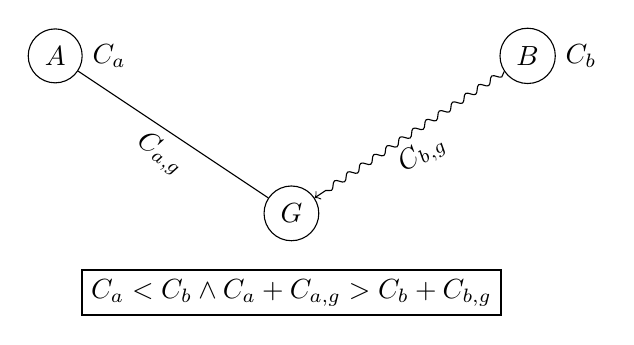
\begin{tikzpicture}[stateS/.style={shape=circle,draw=black},costC/.style={below,sloped,midway},costS/.style={anchor=west}]
\node[stateS] (A) at (-3,0) {$A$};
\node[costS] (cA) at (A.east) {$C_a$};
\node[stateS] (B) at (3,0) {$B$};
\node[costS] (cB) at (B.east) {$C_b$};
\node[stateS] (G) at (0,-2) {$G$};
\node[anchor=north,yshift=-10,shape=rectangle,draw=black,thick] (M) at (G.south) {$C_a<C_b\wedge C_a+C_{a,g}>C_b+C_{b,g}$};
\draw (A) to node[costC]{$C_{a,g}$} (G);
\draw[->,decorate,decoration={snake,amplitude=.4mm,segment length=2mm,post length=1mm}] (B) to node[costC]{$C_{b,g}$} (G);
\end{tikzpicture}
\caption{Algemeen geval van falen bij Uniform Cost Search}
\label{fig:badUniformCost}
\end{figure}
\begin{leftbar}
We passen bovendien dit algoritme toe op ons wegenplan, en bekomen een niet optimaal pad of figuur \ref{fig:uniformCostCity} op pagina \pageref{fig:uniformCostCity}, waar de kost 15 is, in plaats van 13.
\end{leftbar}
Dit algoritme geeft wel in de meeste gevallen al een behoorlijk optimale oplossing. Dit algoritme wordt beschreven in \algref{alg:uniformCost}.
\begin{algorithm}[htb]                      % enter the algorithm environment
\caption{Uniform Cost zoekalgoritme}          % give the algorithm a caption
\label{alg:uniformCost}                           % and a label for \ref{} commands later in the document
\begin{algorithmic}[1]                    % enter the algorithmic environment
\STATE $\queue\leftarrow\mbox{Path containing the root}$
\WHILE{$\notempty{\queue}\wedge\neg\goalreached{\queue}$}
\STATE $r\leftarrow\dequeue{\queue}$
\STATE $R\leftarrow\createnewpaths{r}$
\STATE $\removeloops{R}$
\STATE $\enqueue{\queue,R}$\COMMENT{De plaats doet er niet toe, de $\queue$ wordt nog gesorteerd}
\STATE $\quicksort{\queue,c}$
\ENDWHILE
\IF{$\goalreached{\queue}$}
\RETURN $\success$
\ELSE
\RETURN $\failure$
\ENDIF
\end{algorithmic}
\end{algorithm}
Indien we het loopdetectie-systeem even buiten beschouwing laten in onze tijds- en geheugencomplexiteitsanalyse, bekomen we volgende criteria:
\begin{center}
\begin{tabular}{ll}
\textbf{Compleet}:&Ja\\
\textbf{Snelheid}:&\bigoh{b^d}\\
\textbf{Geheugen}:&\bigoh{b^d}\\
\textbf{Optimaal}:&Nee
\end{tabular}
\end{center}
\subsection{Optimal Uniform Cost Algorithm}
Het \termen{Optimal Uniform Cost Algorithm}, garandeert wel een optimale oplossing, dit wordt gegarandeerd door het \termen{Branch-and-Bound Principe}. Dat principe zegt dat eenmaal we een pad dat naar een doel wijst gevonden hebben, we alle paden met een accumulatieve kost groter dan dat pad niet meer dienen te beschouwen (de kost neemt immers alleen maar toe). Indien onze $\queue$ een pad bevat dat naar een doel wijst, en dit komt als eerste voor, weten we zeker dat dit het optimale pad is. Gebasseerd op deze theorie herschrijven we dus onze terminatieconditie van het Uniform Cost Algorithm. Dit algoritme wordt beschreven in \algref{alg:optimalUniformCost}.
\begin{algorithm}[htb]                      % enter the algorithm environment
\caption{Optimal Uniform Cost zoekalgoritme}          % give the algorithm a caption
\label{alg:optimalUniformCost}                           % and a label for \ref{} commands later in the document
\begin{algorithmic}[1]                    % enter the algorithmic environment
\STATE $\queue\leftarrow\mbox{Path containing the root}$
\WHILE{$\notempty{\queue}\wedge\neg\goalreached{\queue\left[0\right]}$}
\STATE $r\leftarrow\dequeue{\queue}$
\STATE $R\leftarrow\createnewpaths{r}$
\STATE $\removeloops{R}$
\STATE $\enqueue{\queue,R}$\COMMENT{De plaats doet er niet toe, de $\queue$ wordt nog gesorteerd}
\STATE $\quicksort{\queue,c}$
\ENDWHILE
\IF{$\goalreached{\queue\left[0\right]}$}
\RETURN $\success$
\ELSE
\RETURN $\failure$
\ENDIF
\end{algorithmic}
\end{algorithm}
Indien we het loopdetectie-systeem even buiten beschouwing laten in onze tijds- en geheugencomplexiteitsanalyse, bekomen we volgende criteria:
\begin{center}
\begin{tabular}{ll}
\textbf{Compleet}:&Ja\\
\textbf{Snelheid}:&\bigoh{b^d}\\
\textbf{Geheugen}:&\bigoh{b^d}\\
\textbf{Optimaal}:&Ja
\end{tabular}
\end{center}
\begin{leftbar}
Een concrete uitwerking van dit algoritme wordt weergegeven op figuur \ref{fig:optimalUniformCostCity} op pagina \pageref{fig:optimalUniformCostCity}. We merken op dat deze gegarandeerde optimaliteit echter een grote hoeveelheid extra werk kan betekenen (66\% extra werk voor een oplossing die slechts 13\% beter is).
\end{leftbar}
\subsection{Extended Uniform Cost}
Het Optimal Uniform Cost algoritme werkt goed zolang de constraint $c\left(p_i,p_{i+1}\right)>0$ stand houdt, met andere woorden dat de kost tussen elke boog groter is dan 0. Het nadeel van dit zoekalgoritme is echter dat er opnieuw weinig probleem gerelateerde informatie aan te pas komt. Een oplossing bestaat erin een nieuwe functie te defini\"eren: de \termen{Extended Uniform Cost} $f:\Pp\rightarrow\Rr:p\mapsto r=f\left(p\right)$:
\begin{equation}
f\left(p\right)=c\left(p\right)+h\left(p_{\mbox{\small{end state}}}\right)
\end{equation}
Dit is dus de som van de reeds gemaakte kosten $c$, en een schatting $h$ van de nog te maken kosten tot de oplossing. Samen vormt dit dus een schatting van de kosten die we zullen betalen voor een pad naar het doel, met als subpad het huidige pad. Met deze functie kunnen we algoritmen ontwikkelen die gerichter op zoek gaan naar een oplossing, maar waarbij de optimaliteit behouden blijft.
\subsection{Estimate-extended Uniform Cost Algorithm}
Een algoritme die gebruik maakt van de Extended Uniform Cost is het \termen{Estimate-extended Uniform Cost Algorithm}. Dit is een variant op het Optimal Uniform Cost Algorithm, maar waarbij de knopen op de Extended Uniform Cost $f$ gesorteerd worden in plaats van de Uniform Cost $c$. Dit algoritme wordt beschreven in \algref{alg:estimateExtendedUniformCost}.
\begin{algorithm}[htb]                      % enter the algorithm environment
\caption{Estimate-extended Uniform Cost zoekalgoritme}          % give the algorithm a caption
\label{alg:estimateExtendedUniformCost}                           % and a label for \ref{} commands later in the document
\begin{algorithmic}[1]                    % enter the algorithmic environment
\STATE $\queue\leftarrow\mbox{Path containing the root}$
\WHILE{$\notempty{\queue}\wedge\neg\goalreached{\queue\left[0\right]}$}
\STATE $r\leftarrow\dequeue{\queue}$
\STATE $R\leftarrow\createnewpaths{r}$
\STATE $\removeloops{R}$
\STATE $\enqueue{\queue,R}$\COMMENT{De plaats doet er niet toe, de $\queue$ wordt nog gesorteerd}
\STATE $\quicksort{\queue,f}$
\ENDWHILE
\IF{$\goalreached{\queue\left[0\right]}$}
\RETURN $\success$
\ELSE
\RETURN $\failure$
\ENDIF
\end{algorithmic}
\end{algorithm}
Dit algoritme komt tot een optimale oplossing wanneer we echter nog een extra constraint plaatsen op de heuristiek. Als we het terminatiecriterium bekijken moet de meest optimale oplossing op het einde van het algoritme vooraan staan. Eventueel kunnen paden, die op dat moment echter een ongunstige heuristiek hebben, toch nog optimalere oplossingen opleveren. Het zou kunnen gebeuren dat optimale paden uit de boot vallen, indien op dat moment de heuristiek de nog te maken kosten overschat. De oplossing is het stellen dat de heuristiek altijd een \termen{Onderschatting} moet zijn van de nog te nemen kost tot een doel. Met andere woorden:
\begin{equation}
h\left(T\right)\leq c\left(T_{\mbox{\small{end point}}}\ldots\goal\right)
\end{equation}
Over het algemeen presteren deze algoritmen goed indien een goede heuristische functie gekozen wordt. Het berekenen van de functie impliceert echter ook overhead, bijgevolg is de beste heuristiek niet altijd geschikt om te zoeken. Indien we het loopdetectie-systeem even buiten beschouwing laten in onze tijds- en geheugencomplexiteitsanalyse, bekomen we volgende criteria:
\begin{center}
\begin{tabular}{ll}
\textbf{Compleet}:&Ja\\
\textbf{Snelheid}:&\bigoh{b^d}\\
\textbf{Geheugen}:&\bigoh{b^d}\\
\textbf{Optimaal}:&Ja (mits onderschatting)
\end{tabular}
\end{center}
\begin{leftbar}
Een uitgewerkt voorbeeld van Estimate-Extended Uniform Cost Search op het wegenplan wordt beschreven op figuur \ref{fig:estimateExtendedUniformCostCity} op pagina \pageref{fig:estimateExtendedUniformCostCity}.
\end{leftbar}
\subsection{Path Deletion}
Een andere uitbreiding die we kunnen toepassen en die algemeen toepasbaar is, is \termen{Path Deletion}. Bij het genereren van de boom genereren we vaak dezelfde toestand in verschillende takken van de boom (volgens het principe ``vele wegen leiden naar Rome''). We kunnen echter door de evaluatie van \'e\'en van deze staten tot een oplossing komen. Evaluatie van de andere versies leidt alleen maar tot overhead, en enkel de versie van de staat met de tot dan toe laagste cummulatieve kost komt in aanmerking voor een optimale oplossing. Path Deletion verwijdert de paden uit de queue die overhead veroorzaken. Indien er al een pad bestaat met dezelfde eindstaat, en de kost van dat pad is lager, is het niet nodig om de paden met eenzelfde eindpunt maar een hogere kost in de wachtrij te houden. Deze zullen immers altijd een hogere kost behouden. Of meer formeel in \algref{alg:pathDeletion}.
\begin{algorithm}[htb]                      % enter the algorithm environment
\caption{Path Deletion Principe}          % give the algorithm a caption
\label{alg:pathDeletion}                           % and a label for \ref{} commands later in the document
\begin{algorithmic}[1]                    % enter the algorithmic environment
\IF{$P\in\queue\wedge P=\left(\rootR,\ldots,I\right)\wedge Q\in\queue\wedge Q=\left(\rootR,\ldots,I,\ldots\right)\wedge c\left(P\right)\geq c\left(Q\right)$}
\STATE $\delete{\queue,P}$
\ENDIF
\end{algorithmic}
\end{algorithm}
\subsection{A* Search}
Het populairste zoekalgoritme bij uitstek is \termen{A* Search}, die eigenlijk een combinatie is van het beste uit verschillende zoekalgoritmen. A* is een uitbreiding op het Extended Uniform Cost Search Algoritme waarbij men het Branch-and-Bound principe, Heuristische Underestimate en de Redudant Path Deletion uitbreidingen toevoegt. Dit algoritme wordt beschreven in \algref{alg:aStar}. Een uitgewerkt voorbeeld staat op figuur \ref{fig:aStarCity} op pagina \pageref{fig:aStarCity}.
\begin{algorithm}[htb]                      % enter the algorithm environment
\caption{A* zoekalgoritme}          % give the algorithm a caption
\label{alg:aStar}                           % and a label for \ref{} commands later in the document
\begin{algorithmic}[1]                    % enter the algorithmic environment
\STATE $\queue\leftarrow\mbox{Path containing the root}$
\WHILE{$\notempty{\queue}\wedge\neg\goalreached{\queue\left[0\right]}$}
\STATE $r\leftarrow\dequeue{\queue}$
\STATE $R\leftarrow\createnewpaths{r}$
\STATE $\removeloops{R}$
\STATE $\enqueue{\queue,R}$\COMMENT{De plaats doet er niet toe, de $\queue$ wordt nog gesorteerd}
\STATE $\quicksort{\queue,f}$
\STATE\COMMENT{Path Deletion}
\FORALL{$P,Q\in\queue$}
\IF{$P=\left(\rootR,\ldots,I\right)\wedge Q=\left(\rootR,\ldots,I,\ldots\right)\wedge c\left(P\right)\geq c\left(Q\right)$}
\STATE $\delete{\queue,P}$
\ENDIF
\ENDFOR
\ENDWHILE
\IF{$\goalreached{\queue\left[0\right]}$}
\RETURN $\success$
\ELSE
\RETURN $\failure$
\ENDIF
\end{algorithmic}
\end{algorithm}
Vanwege de populariteit van A* zullen we wat dieper ingaan op enkele eigenschappen van A*.
\paragraph{Bewijs van Optimaliteit}
Alvorens we A* kunnen gebruiken, moeten we eerst een bewijs kunnen formuleren die borg staat dat A* altijd tot een optimale oplossing zal komen. Hiervoor maken we gebruik van enkele eigenschappen die we ook formeel aantonen. Hierbij stelt $B$ het meest optimale pad van de bron naar het doel voor.
\begin{theorem}
Voor ieder subpad $p$ van $B$ is de uitgebreide kost van $p$ kleiner of gelijk aan de kost van $B$. $\forall p \mbox{ subpath of } B: f\left(p\right)\leq c\left(B\right)$
\end{theorem}
\begin{proof}
\[
\begin{array}{c}
f\left(p\right)=c\left(p\right)+h\left(p_{\mbox{\small{end point}}}\right)\wedge h\left(p_{\mbox{\small{end point}}}\right)\leq c\left(p_{\mbox{\small{end point}}}\ldots\goal\right)\\
\Downarrow\\
f\left(p\right)\leq c\left(p\right)+c\left(p_{\mbox{\small{end point}}}\ldots\goal\right)=c\left(p,\ldots,\goal\right)=c\left(B\right)
\end{array}
\]
\end{proof}
\begin{theorem}
Tijdens iedere while test van A* bevat de $\queue$ een subpad van $B$
\label{the:astarsubpath}
\end{theorem}
\begin{proof}
\[
\begin{array}{c}
\mbox{bewijs door middel van inductie}:\\\\
\begin{array}{ll}
\mbox{\underline{Initieel:} }&S=\mbox{pad dat de bron bevat } \in\queue\wedge S \mbox{ is een subpad van } B\\
&\Downarrow\\
&\mbox{subpad van }B\in\queue\\\\
\mbox{\underline{Iteratie:} }&\mbox{indien een subpad van $B$ verwijdert wordt}\\\\
&\mbox{- het subpad heeft ten minste een kind (anders bestaat er geen $B$)}\\
&\mbox{- bovendien bevat dat kind geen lus ($B$ bevat geen lus)}\\\\
&\Rightarrow\mbox{Dit kind wordt weer toegevoegd aan de $\queue$}\\
&\Rightarrow\mbox{een subpad van }B\in\queue\\\\
\end{array}
\end{array}
\]
\end{proof}
\begin{corollary}
Voor ieder pad $p$ zodat $f\left(p\right)>c\left(B\right)$, kan $p$ nooit geselecteerd worden (Het zal nooit als eerste in de $\queue$ zitten).
\end{corollary}
\begin{proof}
\[
\begin{array}{c}
\begin{array}{rcl}
\mbox{altijd een subpad $q$ van}&\wedge&f\left(q\right)\leq c\left(B\right)<f\left(p\right)\\
\mbox{$B$ met } f\left(q\right)\leq c\left(B\right)&&\\
&\Downarrow&\\
\multicolumn{3}{c}{\mbox{$p$ wordt nooit geselecteerd}}
\end{array}
\end{array}
\]
\end{proof}
\paragraph{Bewijs van terminatie}
Stel $d$ is een natuurlijk getal $>c\left(B\right)/\delta$ (hierbij is $\delta$ de kleinste kost van alle bogen), en stel $P$ een pad van lengte $d$. In dat geval geldt:
\begin{equation}
f\left(P\right)=c\left(P\right)+h\left(P\right)\geq c\left(P\right)\geq d\cdot\delta>c\left(B\right)=f\left(B\right)
\end{equation}
We weten dus dat het pad $P$ nooit geselecteerd zal worden ($B$ is immers een pad dat het doel bereikt, en heeft een lagere $f$-waarde). Omdat we uitgaan van een eindige vertakkingsfactor $b$, zijn er dus maar een eindig aantal knopen die in de $\queue$ geplaatst kunnen worden. Omdat telkens wanneer we de lus uitvoeren er \'e\'en element uit de $\queue$ gehaald wordt, zal de $\queue$ op een gegeven moment leeg zijn, waardoor de lus doorbroken wordt en het algoritme stopt.
\paragraph{Bewijs van compleetheid}
Door theorema \ref{the:astarsubpath} kunnen we bewijzen dat het pad dat uiteindelijk zal evolueren naar een doel altijd in de $\queue$ zit, bijgevolg zal A* altijd het doel vinden.
\paragraph{Selectiegedrag van A*}
Welke knopen zullen ge\"expandeert worden? We kunnen de impliciete boom onderverdelen in drie verschillende groepen:
\begin{itemize}
 \item \termen{Nooit geselecteerde knopen}: Hierbij is $f\left(p\right)>c\left(B\right)$ of een redundant pad.
 \item \termen{Misschien geselecteerd knopen}: Hierbij is $f\left(p\right)=c\left(B\right)$
 \item \termen{Geselecteerde knopen}: Hierbij is $p\in\queue\wedge p\mbox{ is niet redundant}\wedge f\left(p\right)<c\left(B\right)$
\end{itemize}
\paragraph{Heuristische kracht}
\termen{Heuristical Power} gaat over in welke mate de heuristische functie belangrijk is voor het A* algoritme, en of we twee heuristische functies op de \'e\'en of andere manier kunnen vergelijken met elkaar. Door de constraint dat iedere heuristische functie alleen strikt positieve getallen moet teruggeven, en daarenboven een onderschatting moet zijn van de nog te nemen kost, kunnen we aantonen dat de heuristische functie het A* algoritme in ieder geval niet slechter kan doen presteren dan bijvoorbeeld het Optimal Uniform Cost algoritme. Indien we echter naar een vergelijking tussen twee heuristische functies streven, is het zo dat een functie die bij iedere toestand een grotere waarde retourneert dan zijn tegenhanger per definitie beter is. Met andere woorden:
\begin{equation}
 h_1 \mbox{ is beter dan } h_2\leftrightarrow\forall s\in\Ss:h_1\left(s\right)\geq h_2\left(s\right)
\end{equation}
Dit kunnen we beargumenteren omdat een heuristische functie per definitie een onderschatting moet zijn voor de werkelijke nog te betalen kost, en dus de heuristiek waarschijnlijk realistischer zal zijn. Verder kunnen we ook nog formeel aantonen dat indien $h_1$ beter is dan $h_2$ en er bestaat een pad van de bron naar het doel, dan zal A* met $h_2$ alle knopen evalueren die A* onder $h_1$ ge\"evalueerd zou hebben, met andere woorden A* zal zo goed als altijd langer werken met een slechtere heuristiek dan met een betere, volgens onze definitie van beter.
\subparagraph{Minimale kost paden en monotoniciteit}
Als we \algref{alg:pathDeletion} dichter bekijken zien we een asymmetrie in het algoritme, dit resulteert in het feit dat niet elke redundante knoop ontdekt wordt. Indien we bijvoorbeeld een pad beschouwen $\left(S,A,C,D\right)$ dat bij $C$ een geaccumuleerde kost heeft van $5$, en we expanderen een ander pad zodat er een kind-pad ontstaat $\left(S,B,C\right)$ met een geaccumuleerde kost van $4$ zal het eerste pad niet verwijdert worden (zie figuur \ref{fig:badMonotonicity}, hierbij gebeurt evaluatie als volgt: $S$, $A$, $C$, $D$ en $B$).
\begin{figure}[htb]
\centering
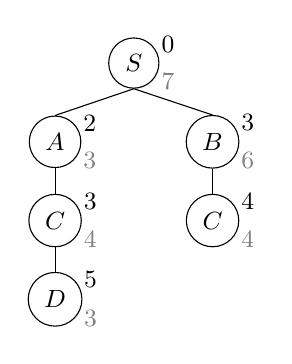
\begin{tikzpicture}[scale=0.5,stateS/.style={shape=circle,draw=black},costC/.style={below,sloped,midway},costS/.style={anchor=west},heurS/.style={gray,anchor=west}]
\node[stateS] (S) at (0,0) {\small $S$};
\node[costS] (cS) at (S.north east) {\small $0$};
\node[heurS] (hS) at (S.south east) {\small $7$};

\node[stateS] (A) at (-2,-2) {\small $A$};
\node[costS] (cA) at (A.north east) {\small $2$};
\node[heurS] (hA) at (A.south east) {\small $3$};

\node[stateS] (C) at (-2,-4) {\small $C$};
\node[costS] (cC) at (C.north east) {\small $3$};
\node[heurS] (hC) at (C.south east) {\small $4$};

\node[stateS] (D) at (-2,-6) {\small $D$};
\node[costS] (cD) at (D.north east) {\small $5$};
\node[heurS] (hD) at (D.south east) {\small $3$};

\node[stateS] (B) at (2,-2) {\small $B$};
\node[costS] (cB) at (B.north east) {\small $3$};
\node[heurS] (hB) at (B.south east) {\small $6$};

\node[stateS] (C2) at (2,-4) {\small $C$};
\node[costS] (cC2) at (C2.north east) {\small $4$};
\node[heurS] (hC2) at (C2.south east) {\small $4$};
\draw (S.south) -- (A.north);
\draw (A.south) -- (C.north);
\draw (C.south) -- (D.north);
\draw (S.south) -- (B.north);
\draw (B.south) -- (C2.north);
\end{tikzpicture}
\caption{Concreet geval van een niet monotone heuristiek}
\label{fig:badMonotonicity}
\end{figure}
Het is immers al het verst uitgebreid, en de kost is niet lager. Deze situatie kan voorkomen indien de heuristiek van $B$ bijvoorbeeld heel hoog was, terwijl deze van $A$ en $C$ veel kleiner waren. We kunnen het Path Deletion algoritme in principe niet al te veel aanpassen zodat het hier ook rekening mee houdt. Dit komt omdat deze knoop al ge\"expandeert is en we dus dubbel werk willen vermijden. Anderzijds kunnen we een constraint opleggen op onze heuristiek zodat deze nooit tot dergelijk situaties kan leiden. Deze constraint heet \termen{Monotoniciteit} of \termen{Monotonicity}. Deze stelt dat indien we een staat $A$ hebben, en $B$ is hiervan een kind, dan moet de heuristische waarde van $A$ kleiner of gelijk zijn aan de heuristische waarde van $B$ en de kost van $A$ naar $B$, of meer formeel:
\begin{equation}
B\mbox{ is een kind van }A\rightarrow h\left(A\right)\leq h\left(B\right)+c\left(A,B\right)
\end{equation}
Opnieuw is deze maatregel redelijk: indien immers niet aan de monotoniciteitsregel wordt voldaan betekent dit dat de heuristiek van $B$ een nog grotere onderschatting van het pad is dan de heuristiek van $A$. We weten na de heuristiek van $A$ te hebben ge\"evalueerd reeds dat we meer kosten zullen hebben dan die heuristiek. Indien $B$ een grotere onderschatting is, weten we eigenlijk helemaal niets nieuws. De heuristiek van $B$ zou in dat geval informatieloos zijn. A* zal indien we de monotoniciteitsregel volgen altijd een knoop selecteren met het meest effici\"entste pad tot de knoop. Verder kunnen we ook het Redudant Path algoritme optimaliseren onder deze voorwaarde, zoals in \algref{alg:optimalPathDeletion}.
\begin{algorithm}[htb]                      % enter the algorithm environment
\caption{Geoptimaliseerd Path Deletion Principe}          % give the algorithm a caption
\label{alg:optimalPathDeletion}                           % and a label for \ref{} commands later in the document
\begin{algorithmic}[1]                    % enter the algorithmic environment
\STATE ${\mathfrak H}\leftarrow\varnothing$
\IF{A* selecteerd een pad $p$}
\STATE $s\leftarrow p_{\mbox{end state}}$
\IF{$\hashtablecontains{{\mathfrak H},s}$}
\STATE do not evaluate $p$
\ELSE
\STATE $\inserthashtable{{\mathfrak H},s}$
\ENDIF
\ENDIF
\end{algorithmic}
\end{algorithm}
Hierdoor wordt path deletion vrijwel altijd gedaan in \bigoh{1}.
\paragraph{Pathmax}
\termen{Pathmax} is een variant van A* die deze monotoniciteitsregel afdwingt. Dit kan op verschillende manieren gedaan worden:
\begin{itemize}
 \item Corrigeren van de waarde van $f$: Indien $B$ een kind is van $A$ en $f\left(S,\ldots,A,B\right)<f\left(S,\ldots,A,\right)$ dan nemen we voor $f\left(S,\ldots,A,B\right)$ dezelfde waarde als $f\left(S,\ldots,A\right)$.
 \item $f$ herdefini\"eren: we genereren zelf een functie $f'$ die we defini\"eren als
\begin{equation}
f'\left(S,\ldots,A,B\right)=\mathfunc{max}{c\left(S,\ldots,A,B\right)+h\left(B\right),f'\left(S,\ldots,A\right)}
\end{equation}
\end{itemize}
\subsection{Iterative Deepening A* (IDA*)}
Een variant van A* is \termen{Iterative Deepening A*} of afgekort \termen{IDA*}. Deze heeft tot doel het geheugengebruik van A* meer onder controle te houden (we kunnen A* immers in de verte vergelijken met breedte-eerst, en dit algoritme is niet zuinig met geheugen). Net als Iterative Deepening een beperking op de diepte stelt voor Depth-First, stelt IDA* een beperking op de $f$ waarde. Indien we verwachten dat de oplossing bijvoorbeeld een $f$-waarde zal hebben van 100 zal het algoritme de kinderen van ge\"evalueerde knopen niet meer opslaan indien deze een $f$-waarde groter hebben dan 100. Uiteraard kan het gebeuren dat onze schatting niet toereikend was om tot een oplossing te komen, in dat geval wordt de $f$-waarde verhoogt en voeren \termen{$f$-limited Search} opnieuw uit. Meestal wordt als begin $f$-waarde de $f$-waarde van de bron $f\left(S\right)$ genomen, al dan niet vermenigvuldigt met een factor. Verder wordt de $f$-limiet meestal verhoogt naar de minimale $f$ die groter was dan de $f$-limiet. Dit wordt beschreven in \algref{alg:iterativeDeepeningAStar}.
\begin{algorithm}[htb]                      % enter the algorithm environment
\caption{Iterative Deepening A* zoekalgoritme}          % give the algorithm a caption
\label{alg:iterativeDeepeningAStar}                           % and a label for \ref{} commands later in the document
\begin{algorithmic}[1]                    % enter the algorithmic environment
\STATE $\fbound\leftarrow f\left(S\right)$\COMMENT{Or another $\fbound$-offset value}
\STATE $\queue\leftarrow\varnothing$
\WHILE{$\neg\goalreached{\queue}$}
\STATE\COMMENT{Begin $f$-limited Search}
\STATE $\queue\leftarrow\mbox{Path containing the root}$
\STATE $\fnew\leftarrow\infty$
\WHILE{$\notempty{\queue}$}
\STATE $r\leftarrow\dequeue{\queue}$
\STATE $R\leftarrow\createnewpaths{r}$
\STATE $\removeloops{R}$
\STATE $\fnew\leftarrow\minM{}{\fnew,f\left(\minM{f}{\select{R,\left(R_i\right)>\fbound}}\right)}$
\STATE $\removeif{R,f\left(R_i\right)>\fbound}$
\STATE\COMMENT{Because we will evaluate them all the nodes lower than}
\STATE\COMMENT{a certain $f$-value we don't have to sort them in any order}
\STATE $\enqueuefront{\queue,R}$
\STATE\COMMENT{Path Deletion}
\IF{$P,Q\in\queue\wedge P=\left(\rootR,\ldots,I\right)\wedge Q=\left(\rootR,\ldots,I,\ldots\right)\wedge c\left(P\right)\geq c\left(Q\right)$}
\STATE $\delete{\queue,P}$
\ENDIF
\ENDWHILE
\STATE\COMMENT{Einde $f$-limited Search}
\STATE $\fbound\leftarrow\fnew$
\ENDWHILE
\end{algorithmic}
\end{algorithm}
Indien we het loopdetectie- en path deletion-systeem even buiten beschouwing laten in onze tijds- en geheugencomplexiteitsanalyse, bekomen we volgende criteria:
\begin{center}
\begin{tabular}{ll}
\textbf{Compleet}:&Ja\\
\textbf{Snelheid}:&\bigoh{N^2}\\
\textbf{Geheugen}:&\bigoh{b\cdot c\left(B\right)/\delta}\\
\textbf{Optimaal}:&Ja\\
\end{tabular}
\end{center}
\subsection{Simplified Memory-bounded A* (SMA*)}
Een gelijkaardig effect probeert \termen{Simplified Memory-bounded A*} (of kortweg \termen{SMA*}) te bereiken. Hierbij is het geheugen echter begrensd, en moeten we proberen om in deze beperkende omstandigheden toch een optimale oplossing te vinden. Dit behoorlijke complexe algoritme heeft als basisidee dat indien het geheugen vol is, en we moeten een knoop evalueren, de knopen met de hoogste $f$-waarde tijdelijk uit het geheugen worden gelaten. Om echter geen overbodig werkt te doen in het herberekenen van alle knopen veranderen we de $f$-waarde van de ouder. De ouder van een te verwijderen knoop houdt telkens de beste (laagste) $f$-waarde van van zijn kinderen bij. Deze $f$-waardes spelen vervolgens nog een rol om de knopen opnieuw te evalueren, en te zoeken naar een eventueel doel.
\paragraph{}Een belangrijk aspect hierbij is dat kinderen \'e\'en voor \'e\'en gegenereerd worden om geen \termen{Memory Overflow} te bekomen. Indien het geheugen vol is, moet een knoop wijken voor de te genereren knoop. Verder kan dit algoritme uiteraard geen doelen vinden waarbij het pad naar het doel meer geheugen vereist dan er beschikbaar is. Het algoritme is echter wel compleet wanneer er voldoende geheugen voorradig is.%Dit wordt formeel beschreven in \algref{alg:simplifiedMemoryBoundedAStar}.
%\begin{algorithm}[htb]                      % enter the algorithm environment
%\caption{Simplified Memory-bounded A* zoekalgoritme}          % give the algorithm a caption
%\label{alg:simplifiedMemoryBoundedAStar}                           % and a label for \ref{} commands later in the document
%\begin{algorithmic}[1]                    % enter the algorithmic environment
%\STATE $\queue\leftarrow\mbox{Path containing the root}$
%\WHILE{$\notempty{\queue}\wedge\neg\goalreached{\queue\left[0\right]}$}
%\STATE $r\leftarrow\queue\left[0\right]$\COMMENT{The node still remains in the $\queue$}
%\STATE $r'\leftarrow\mathcommand{nextSuccessor}{r}$
%\STATE $f\left(r'\right)\leftarrow\mathcommand{max}{f\left(r\right),f\left(r'\right)}$
%\STATE $\enqueue{\queue,r'}$\COMMENT{Doesn't matter where}
%\ENDWHILE
%\IF{$\goalreached{\queue\left[0\right]}$}
%\STATE $\quicksort{\queue,f}$
%\RETURN $\success$
%\ELSE
%\RETURN $\failure$
%\ENDIF
%\end{algorithmic}
%\end{algorithm}
%Indien we het loopdetectie- en path deletion-systeem even buiten beschouwing laten in onze tijds- en geheugencomplexiteitsanalyse, bekomen we volgende criteria:
%\begin{center}
%\begin{tabular}{ll}
%\textbf{Completeness}:&Ja\\
%\textbf{Speed}:&\bigoh{b^d}\\
%\textbf{Memory}:&\bigoh{1}\\
%\end{tabular}
%\end{center}
\section{Besluitende commentaren}
\subsection{Niet Optimale Varianten}
Tot dusver zochten we altijd naar optimale oplossingen, soms is het echter beter om niet de meest optimale oplossing te zoeken indien dit tijdswinst kan opleveren. Indien we gebruik maken van \termen{Non-optimal variants}, is dit meestal door de heuristiek aan te passen. Deze zullen meestal het onderschattings-aspect achterwege laten, en worden meestal \termen{Non-admissible heuristics} genoemd. Een andere mogelijkheid is het toepassen van een ander zoekalgoritme. Een variant van A*, het \termen{Non-admissible A* Search Algorithm} is hier een voorbeeld van. Hierbij wordt $f$ als volgt gedefinieerd:
\begin{equation}
f\left(p\right)=\left.\omega\cdot c\left(p\right)+h\left(p_{\mbox{\small{end state}}}\right)\ \ \ \ \right|\omega\in\left[0,1\right]
\end{equation}
Met $\omega$ als een parameter. Indien $\omega=1$ verkrijgen we opnieuw het A* algoritme, indien we $\omega=0$ nemen bekomen we opnieuw Greedy Search.
\subsection{Complexiteit in het algemeen}
Bij nature is het vinden van een optimaal pad dat naar een oplossing voor een dergelijke probleem NP-compleet. Er bestaan echter wel parallelle\footnote{Algoritmen die we kunnen uitvoeren op bijvoorbeeld vector-, DNA- en kwantumcomputers met massaparallellisme.} algoritmen die in polynomiale tijd kunnen werken.%Deze algoritmen zijn echter over het algemeen alleen toepasbaar op kwantumcomputers.
\paragraph{}Meestal leidt dit tot een trade-off waarbij we de optimaliteit reduceren tot een behoorlijke optimale oplossing en hierbij een grote hoeveelheid tijd besparen naar het zoeken van de oplossing. Een voorbeeld hierbij is het instellen van $\omega$ bij Non-admissible A*: hoe meer $\omega$ naar $1$ gaat, hoe meer we in de buurt van een optimale oplossing komen.
\section{Samenvatting}
\label{app:SearchMethods}
\begin{table}[H]
\centering
\begin{tabular}{l|llll|l}
\hline
\textbf{Name}&\textbf{Compleet}&\textbf{Optimaal}&\textbf{Snelheid}&\textbf{Geheugen}&\textbf{Alg.(p.)}\\\hline
\hline
\multicolumn{6}{l}{\textbf{Blind Search}}\\\hline
- Depth First&Ja&Nee&\bigoh{b^d}&\bigoh{b\cdot d}&\ref{alg:depthFirst}(\pageref{alg:depthFirst})\\\hline
- Breadth First&Ja&Nee&\bigoh{b^m}&\bigoh{b^m}&\ref{alg:breadthFirst}(\pageref{alg:breadthFirst})\\\hline
- Neen-Deterministic&Ja&Nee&\bigoh{b^d}&\bigoh{b^d}&\ref{alg:nonDeterministic}(\pageref{alg:nonDeterministic})\\\hline
- Iterative Deepening&Ja&Nee&\bigoh{b^m}&\bigoh{b\cdot m}&\ref{alg:iterativeDeepening}(\pageref{alg:iterativeDeepening})\\\hline
- Bi-Direction Search&Ja&Nee&\bigoh{b^{m/2}}&\bigoh{b^{m/2}}&\ref{alg:biDirectional}(\pageref{alg:biDirectional})\\\hline
\multicolumn{6}{l}{\textbf{Heuristic Search}}\\\hline
- Hill Climbing&Ja&Nee&\bigoh{b^d}&\bigoh{b\cdot d}&\ref{alg:hillClimbing}(\pageref{alg:hillClimbing})\\\hline
- Beam Search&Nee&Nee&\bigoh{w\cdot m}&\bigoh{w}&\ref{alg:beamSearch}(\pageref{alg:beamSearch})\\\hline
- Hill Climbing 2&Nee&Nee&\bigoh{m}&\bigoh{b}&\ref{alg:hillClimbing2}(\pageref{alg:hillClimbing2})\\\hline
- Greedy Search&Ja&Nee&\bigoh{b^d}&\bigoh{b^d}&\ref{alg:greedy}(\pageref{alg:greedy})\\\hline
\multicolumn{6}{l}{\textbf{Optimal Search}}\\\hline
- Uniform Cost&Ja&Nee&\bigoh{b^d}&\bigoh{b^d}&\ref{alg:uniformCost}(\pageref{alg:uniformCost})\\\hline
- Optimal Uniform Cost&Ja&Ja&\bigoh{b^d}&\bigoh{b^d}&\ref{alg:optimalUniformCost}(\pageref{alg:optimalUniformCost})\\\hline
- Estimate-extended Uniform Cost&Ja&Ja&\bigoh{b^d}&\bigoh{b^d}&\ref{alg:estimateExtendedUniformCost}(\pageref{alg:estimateExtendedUniformCost})\\\hline
- A*&Ja&Ja&\bigoh{b^d}&\bigoh{b^d}&\ref{alg:aStar}(\pageref{alg:aStar})\\\hline
- Iterative Deepening A*&Ja&Ja&\bigoh{N^2}&\bigoh{b\cdot c\left(B\right)/\delta}&\ref{alg:iterativeDeepeningAStar}(\pageref{alg:iterativeDeepeningAStar})\\\hline
- Simplified Memory-bounded A*&Ja&Ja&\bigoh{b^d}&\bigoh{1}&\\\hline%\ref{alg:simplifiedMemoryBoundedAStar}(\pageref{alg:simplifiedMemoryBoundedAStar})
\end{tabular}
\caption{Samenvatting van de zoekmethodes}
\end{table}
Een samenvattend schema is te vinden in appendix \ref{app:schemaSearch} op pagina \pageref{app:schemaSearch}.
\newpage
\section{Toepassingen van de zoekalgoritmen (Afbeeldingen)}
\label{ss:cityFigures}
\subsection{Blind Search Methods}
\begin{figure}[H]
\centering
\subfigure{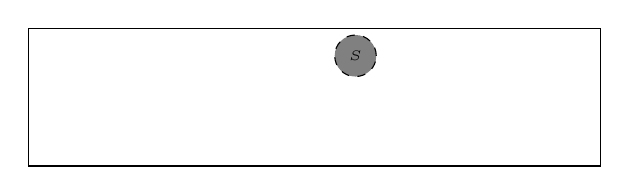
\begin{tikzpicture}[xscale=0.7,yscale=1.4,city/.style={shape=circle,draw=black},costc/.style={anchor=south east},heurh/.style={anchor=north east,gray},cityG/.style={city,very thick},cityM/.style={city,fill=gray}]
\def\dy{-0.75};
\def\dxa{4.75};
\def\dxb{2.875};
\def\dxc{1.125};
\def\dxd{0.75};
\def\dxe{0.75};

\draw (-0.5*\dxa-0.5*\dxb-\dxc-1,0.25) rectangle (0.5*\dxa+0.5*\dxb+\dxc-0.5,1*\dy-0.25);

\node[cityM,dashed] (S) at (0,0) {\tiny $S$};

\end{tikzpicture}}
\subfigure{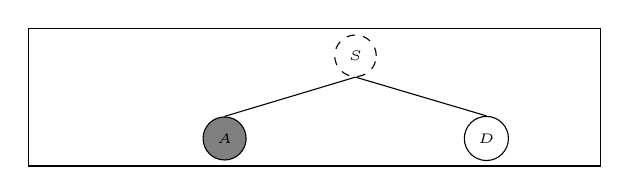
\begin{tikzpicture}[xscale=0.7,yscale=1.4,city/.style={shape=circle,draw=black},costc/.style={anchor=south east},heurh/.style={anchor=north east,gray},cityG/.style={city,very thick},cityM/.style={city,fill=gray}]
\def\dy{-0.75};
\def\dxa{4.75};
\def\dxb{2.875};
\def\dxc{1.125};
\def\dxd{0.75};
\def\dxe{0.75};

\draw (-0.5*\dxa-0.5*\dxb-\dxc-1,0.25) rectangle (0.5*\dxa+0.5*\dxb+\dxc-0.5,1*\dy-0.25);

\node[city,dashed] (S) at (0,0) {\tiny $S$};

\node[cityM] (A) at (-0.5*\dxa,\dy) {\tiny $A$};
\draw (S.south) -- (A.north);
\node[city] (D) at (0.5*\dxa,\dy) {\tiny $D$};
\draw (S.south) -- (D.north);

\end{tikzpicture}}
\subfigure{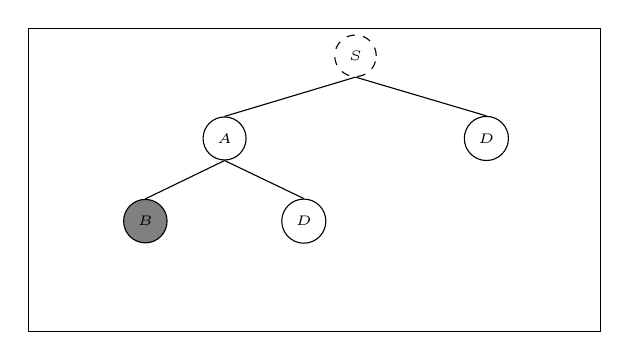
\begin{tikzpicture}[xscale=0.7,yscale=1.4,city/.style={shape=circle,draw=black},costc/.style={anchor=south east},heurh/.style={anchor=north east,gray},cityG/.style={city,very thick},cityM/.style={city,fill=gray}]
\def\dy{-0.75};
\def\dxa{4.75};
\def\dxb{2.875};
\def\dxc{1.125};
\def\dxd{0.75};
\def\dxe{0.75};

\draw (-0.5*\dxa-0.5*\dxb-\dxc-1,0.25) rectangle (0.5*\dxa+0.5*\dxb+\dxc-0.5,3*\dy-0.25);

\node[city,dashed] (S) at (0,0) {\tiny $S$};

\node[city] (A) at (-0.5*\dxa,\dy) {\tiny $A$};
\draw (S.south) -- (A.north);
\node[city] (D) at (0.5*\dxa,\dy) {\tiny $D$};
\draw (S.south) -- (D.north);

\node[cityM] (B) at (-0.5*\dxa-0.5*\dxb,2*\dy) {\tiny $B$};
\draw (A.south) -- (B.north);
\node[city] (D2) at (-0.5*\dxa+0.5*\dxb,2*\dy) {\tiny $D$};
\draw (A.south) -- (D2.north);
\end{tikzpicture}}
\subfigure{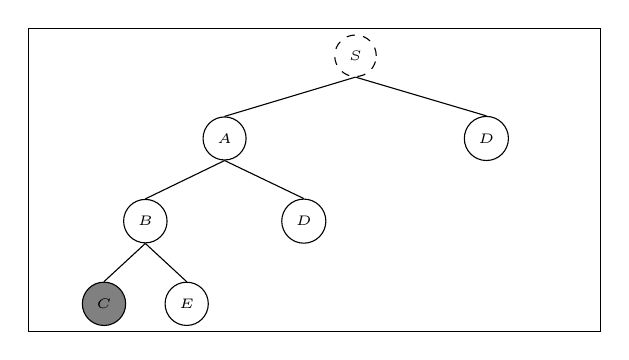
\begin{tikzpicture}[xscale=0.7,yscale=1.4,city/.style={shape=circle,draw=black},costc/.style={anchor=south east},heurh/.style={anchor=north east,gray},cityG/.style={city,very thick},cityM/.style={city,fill=gray}]
\def\dy{-0.75};
\def\dxa{4.75};
\def\dxb{2.875};
\def\dxc{1.125};
\def\dxd{0.75};
\def\dxe{0.75};

\draw (-0.5*\dxa-0.5*\dxb-\dxc-1,0.25) rectangle (0.5*\dxa+0.5*\dxb+\dxc-0.5,3*\dy-0.25);
\def\dxc{1.5};

\node[city,dashed] (S) at (0,0) {\tiny $S$};

\node[city] (A) at (-0.5*\dxa,\dy) {\tiny $A$};
\draw (S.south) -- (A.north);
\node[city] (D) at (0.5*\dxa,\dy) {\tiny $D$};
\draw (S.south) -- (D.north);

\node[city] (B) at (-0.5*\dxa-0.5*\dxb,2*\dy) {\tiny $B$};
\draw (A.south) -- (B.north);
\node[city] (D2) at (-0.5*\dxa+0.5*\dxb,2*\dy) {\tiny $D$};
\draw (A.south) -- (D2.north);

\node[cityM] (C) at (-0.5*\dxa-0.5*\dxb-0.5*\dxc,3*\dy) {\tiny $C$};
\draw (B.south) -- (C.north);
\node[city] (E2) at (-0.5*\dxa-0.5*\dxb+0.5*\dxc,3*\dy) {\tiny $E$};
\draw (B.south) -- (E2.north);
\end{tikzpicture}}
\subfigure{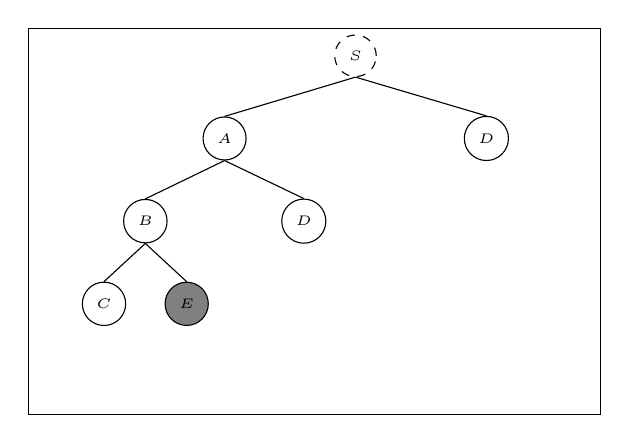
\begin{tikzpicture}[xscale=0.7,yscale=1.4,city/.style={shape=circle,draw=black},costc/.style={anchor=south east},heurh/.style={anchor=north east,gray},cityG/.style={city,very thick},cityM/.style={city,fill=gray}]
\def\dy{-0.75};
\def\dxa{4.75};
\def\dxb{2.875};
\def\dxc{1.125};
\def\dxd{0.75};
\def\dxe{0.75};

\draw (-0.5*\dxa-0.5*\dxb-\dxc-1,0.25) rectangle (0.5*\dxa+0.5*\dxb+\dxc-0.5,4*\dy-0.25);
\def\dxc{1.5};

\node[city,dashed] (S) at (0,0) {\tiny $S$};

\node[city] (A) at (-0.5*\dxa,\dy) {\tiny $A$};
\draw (S.south) -- (A.north);
\node[city] (D) at (0.5*\dxa,\dy) {\tiny $D$};
\draw (S.south) -- (D.north);

\node[city] (B) at (-0.5*\dxa-0.5*\dxb,2*\dy) {\tiny $B$};
\draw (A.south) -- (B.north);
\node[city] (D2) at (-0.5*\dxa+0.5*\dxb,2*\dy) {\tiny $D$};
\draw (A.south) -- (D2.north);

\node[city] (C) at (-0.5*\dxa-0.5*\dxb-0.5*\dxc,3*\dy) {\tiny $C$};
\draw (B.south) -- (C.north);
\node[cityM] (E2) at (-0.5*\dxa-0.5*\dxb+0.5*\dxc,3*\dy) {\tiny $E$};
\draw (B.south) -- (E2.north);
\end{tikzpicture}}
\subfigure{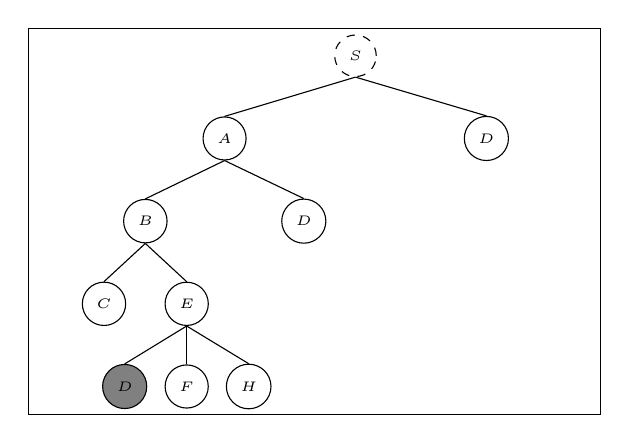
\begin{tikzpicture}[xscale=0.7,yscale=1.4,city/.style={shape=circle,draw=black},costc/.style={anchor=south east},heurh/.style={anchor=north east,gray},cityG/.style={city,very thick},cityM/.style={city,fill=gray}]
\def\dy{-0.75};
\def\dxa{4.75};
\def\dxb{2.875};
\def\dxc{1.125};
\def\dxd{1.125};
\def\dxe{0.75};

\draw (-0.5*\dxa-0.5*\dxb-\dxc-1,0.25) rectangle (0.5*\dxa+0.5*\dxb+\dxc-0.5,4*\dy-0.25);
\def\dxc{1.5};

\node[city,dashed] (S) at (0,0) {\tiny $S$};

\node[city] (A) at (-0.5*\dxa,\dy) {\tiny $A$};
\draw (S.south) -- (A.north);
\node[city] (D) at (0.5*\dxa,\dy) {\tiny $D$};
\draw (S.south) -- (D.north);

\node[city] (B) at (-0.5*\dxa-0.5*\dxb,2*\dy) {\tiny $B$};
\draw (A.south) -- (B.north);
\node[city] (D2) at (-0.5*\dxa+0.5*\dxb,2*\dy) {\tiny $D$};
\draw (A.south) -- (D2.north);

\node[city] (C) at (-0.5*\dxa-0.5*\dxb-0.5*\dxc,3*\dy) {\tiny $C$};
\draw (B.south) -- (C.north);
\node[city] (E2) at (-0.5*\dxa-0.5*\dxb+0.5*\dxc,3*\dy) {\tiny $E$};
\draw (B.south) -- (E2.north);

\node[cityM] (D3) at (-0.5*\dxa-0.5*\dxb+0.5*\dxc-\dxd,4*\dy) {\tiny $D$};
\draw (E2.south) -- (D3.north);
\node[city] (F2) at (-0.5*\dxa-0.5*\dxb+0.5*\dxc,4*\dy) {\tiny $F$};
\draw (E2.south) -- (F2.north);
\node[city] (H2) at (-0.5*\dxa-0.5*\dxb+0.5*\dxc+\dxd,4*\dy) {\tiny $H$};
\draw (E2.south) -- (H2.north);
\end{tikzpicture}}
\subfigure{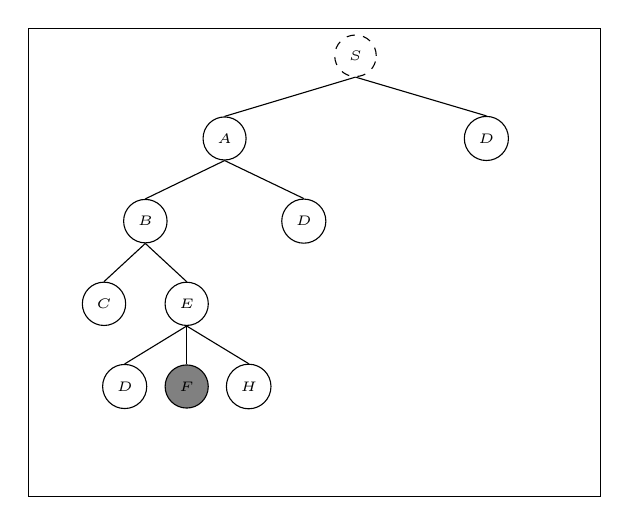
\begin{tikzpicture}[xscale=0.7,yscale=1.4,city/.style={shape=circle,draw=black},costc/.style={anchor=south east},heurh/.style={anchor=north east,gray},cityG/.style={city,very thick},cityM/.style={city,fill=gray}]
\def\dy{-0.75};
\def\dxa{4.75};
\def\dxb{2.875};
\def\dxc{1.125};
\def\dxd{1.125};
\def\dxe{0.75};

\draw (-0.5*\dxa-0.5*\dxb-\dxc-1,0.25) rectangle (0.5*\dxa+0.5*\dxb+\dxc-0.5,5*\dy-0.25);
\def\dxc{1.5};

\node[city,dashed] (S) at (0,0) {\tiny $S$};

\node[city] (A) at (-0.5*\dxa,\dy) {\tiny $A$};
\draw (S.south) -- (A.north);
\node[city] (D) at (0.5*\dxa,\dy) {\tiny $D$};
\draw (S.south) -- (D.north);

\node[city] (B) at (-0.5*\dxa-0.5*\dxb,2*\dy) {\tiny $B$};
\draw (A.south) -- (B.north);
\node[city] (D2) at (-0.5*\dxa+0.5*\dxb,2*\dy) {\tiny $D$};
\draw (A.south) -- (D2.north);

\node[city] (C) at (-0.5*\dxa-0.5*\dxb-0.5*\dxc,3*\dy) {\tiny $C$};
\draw (B.south) -- (C.north);
\node[city] (E2) at (-0.5*\dxa-0.5*\dxb+0.5*\dxc,3*\dy) {\tiny $E$};
\draw (B.south) -- (E2.north);

\node[city] (D3) at (-0.5*\dxa-0.5*\dxb+0.5*\dxc-\dxd,4*\dy) {\tiny $D$};
\draw (E2.south) -- (D3.north);
\node[cityM] (F2) at (-0.5*\dxa-0.5*\dxb+0.5*\dxc,4*\dy) {\tiny $F$};
\draw (E2.south) -- (F2.north);
\node[city] (H2) at (-0.5*\dxa-0.5*\dxb+0.5*\dxc+\dxd,4*\dy) {\tiny $H$};
\draw (E2.south) -- (H2.north);
\end{tikzpicture}}
\subfigure{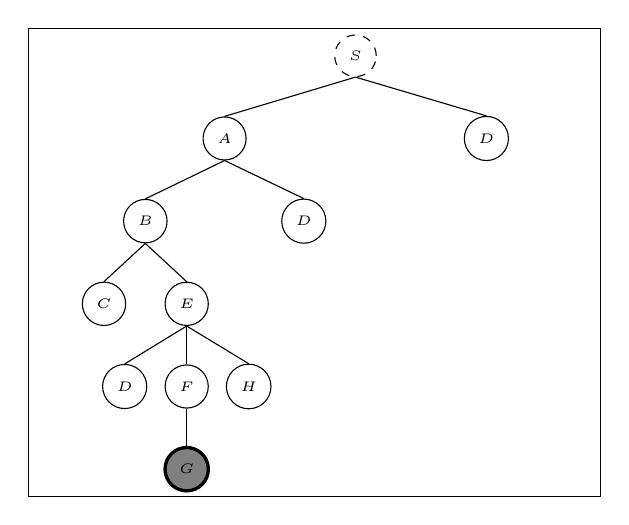
\begin{tikzpicture}[xscale=0.7,yscale=1.4,city/.style={shape=circle,draw=black},costc/.style={anchor=south east},heurh/.style={anchor=north east,gray},cityG/.style={city,very thick},cityM/.style={city,fill=gray},cityMG/.style={cityM,very thick},cityM/.style={city,fill=gray}]
\def\dy{-0.75};
\def\dxa{4.75};
\def\dxb{2.875};
\def\dxc{1.125};
\def\dxd{1.125};
\def\dxe{0.75};

\draw (-0.5*\dxa-0.5*\dxb-\dxc-1,0.25) rectangle (0.5*\dxa+0.5*\dxb+\dxc-0.5,5*\dy-0.25);
\def\dxc{1.5};

\node[city,dashed] (S) at (0,0) {\tiny $S$};

\node[city] (A) at (-0.5*\dxa,\dy) {\tiny $A$};
\draw (S.south) -- (A.north);
\node[city] (D) at (0.5*\dxa,\dy) {\tiny $D$};
\draw (S.south) -- (D.north);

\node[city] (B) at (-0.5*\dxa-0.5*\dxb,2*\dy) {\tiny $B$};
\draw (A.south) -- (B.north);
\node[city] (D2) at (-0.5*\dxa+0.5*\dxb,2*\dy) {\tiny $D$};
\draw (A.south) -- (D2.north);

\node[city] (C) at (-0.5*\dxa-0.5*\dxb-0.5*\dxc,3*\dy) {\tiny $C$};
\draw (B.south) -- (C.north);
\node[city] (E2) at (-0.5*\dxa-0.5*\dxb+0.5*\dxc,3*\dy) {\tiny $E$};
\draw (B.south) -- (E2.north);

\node[city] (D3) at (-0.5*\dxa-0.5*\dxb+0.5*\dxc-\dxd,4*\dy) {\tiny $D$};
\draw (E2.south) -- (D3.north);
\node[city] (F2) at (-0.5*\dxa-0.5*\dxb+0.5*\dxc,4*\dy) {\tiny $F$};
\draw (E2.south) -- (F2.north);
\node[city] (H2) at (-0.5*\dxa-0.5*\dxb+0.5*\dxc+\dxd,4*\dy) {\tiny $H$};
\draw (E2.south) -- (H2.north);

\node[cityMG] (G3) at (-0.5*\dxa-0.5*\dxb+0.5*\dxc,5*\dy) {\tiny $G$};
\draw (F2.south) -- (G3.north);
\end{tikzpicture}}
\caption{Depth-First toegepast op het wegenplan}
\label{fig:depthFirstCity}
\end{figure}
\begin{figure}[H]
\centering
\subfigure{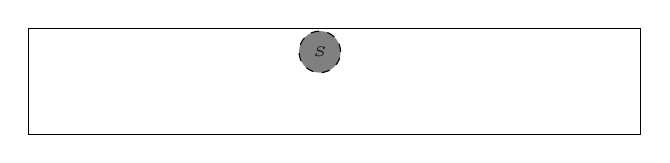
\begin{tikzpicture}[xscale=0.75,yscale=1,city/.style={shape=circle,draw=black},costc/.style={anchor=south east},heurh/.style={anchor=north east,gray},cityG/.style={city,very thick},cityM/.style={city,fill=gray}]
\def\dy{-0.75};
\def\dxa{4.75};
\def\dxb{2.875};
\def\dxc{1.125};
\def\dxd{0.75};
\def\dxe{0.75};

\draw (-0.5*\dxa-0.5*\dxb-\dxc,0.3) rectangle (0.5*\dxa+0.5*\dxb+\dxc+0.5,1*\dy-0.3);

\node[cityM,dashed] (S) at (0,0) {\tiny $S$};
\end{tikzpicture}}
\subfigure{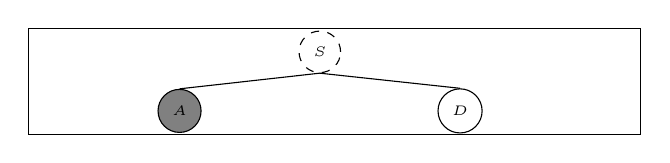
\begin{tikzpicture}[xscale=0.75,yscale=1,city/.style={shape=circle,draw=black},costc/.style={anchor=south east},heurh/.style={anchor=north east,gray},cityG/.style={city,very thick},cityM/.style={city,fill=gray}]
\def\dy{-0.75};
\def\dxa{4.75};
\def\dxb{2.875};
\def\dxc{1.125};
\def\dxd{0.75};
\def\dxe{0.75};

\draw (-0.5*\dxa-0.5*\dxb-\dxc,0.3) rectangle (0.5*\dxa+0.5*\dxb+\dxc+0.5,1*\dy-0.3);

\node[city,dashed] (S) at (0,0) {\tiny $S$};

\node[cityM] (A) at (-0.5*\dxa,\dy) {\tiny $A$};
\draw (S.south) -- (A.north);
\node[city] (D) at (0.5*\dxa,\dy) {\tiny $D$};
\draw (S.south) -- (D.north);
\end{tikzpicture}}
\subfigure{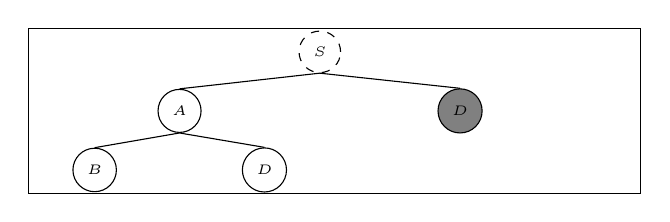
\begin{tikzpicture}[xscale=0.75,yscale=1,city/.style={shape=circle,draw=black},costc/.style={anchor=south east},heurh/.style={anchor=north east,gray},cityG/.style={city,very thick},cityM/.style={city,fill=gray}]
\def\dy{-0.75};
\def\dxa{4.75};
\def\dxb{2.875};
\def\dxc{1.125};
\def\dxd{0.75};
\def\dxe{0.75};

\draw (-0.5*\dxa-0.5*\dxb-\dxc,0.3) rectangle (0.5*\dxa+0.5*\dxb+\dxc+0.5,2*\dy-0.3);

\node[city,dashed] (S) at (0,0) {\tiny $S$};

\node[city] (A) at (-0.5*\dxa,\dy) {\tiny $A$};
\draw (S.south) -- (A.north);
\node[cityM] (D) at (0.5*\dxa,\dy) {\tiny $D$};
\draw (S.south) -- (D.north);

\node[city] (B) at (-0.5*\dxa-0.5*\dxb,2*\dy) {\tiny $B$};
\draw (A.south) -- (B.north);
\node[city] (D2) at (-0.5*\dxa+0.5*\dxb,2*\dy) {\tiny $D$};
\draw (A.south) -- (D2.north);
\end{tikzpicture}}
\subfigure{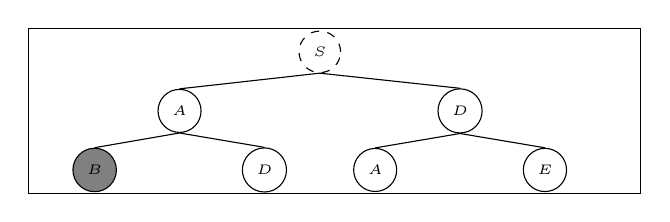
\begin{tikzpicture}[xscale=0.75,yscale=1,city/.style={shape=circle,draw=black},costc/.style={anchor=south east},heurh/.style={anchor=north east,gray},cityG/.style={city,very thick},cityM/.style={city,fill=gray}]
\def\dy{-0.75};
\def\dxa{4.75};
\def\dxb{2.875};
\def\dxc{1.125};
\def\dxd{0.75};
\def\dxe{0.75};

\draw (-0.5*\dxa-0.5*\dxb-\dxc,0.3) rectangle (0.5*\dxa+0.5*\dxb+\dxc+0.5,2*\dy-0.3);

\node[city,dashed] (S) at (0,0) {\tiny $S$};

\node[city] (A) at (-0.5*\dxa,\dy) {\tiny $A$};
\draw (S.south) -- (A.north);
\node[city] (D) at (0.5*\dxa,\dy) {\tiny $D$};
\draw (S.south) -- (D.north);

\node[cityM] (B) at (-0.5*\dxa-0.5*\dxb,2*\dy) {\tiny $B$};
\draw (A.south) -- (B.north);
\node[city] (D2) at (-0.5*\dxa+0.5*\dxb,2*\dy) {\tiny $D$};
\draw (A.south) -- (D2.north);
\node[city] (A2) at (0.5*\dxa-0.5*\dxb,2*\dy) {\tiny $A$};
\draw (D.south) -- (A2.north);
\node[city] (E) at (0.5*\dxa+0.5*\dxb,2*\dy) {\tiny $E$};
\draw (D.south) -- (E.north);
\end{tikzpicture}}
\subfigure{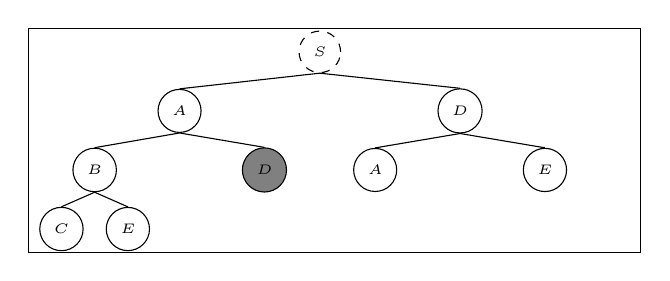
\begin{tikzpicture}[xscale=0.75,yscale=1,city/.style={shape=circle,draw=black},costc/.style={anchor=south east},heurh/.style={anchor=north east,gray},cityG/.style={city,very thick},cityM/.style={city,fill=gray}]
\def\dy{-0.75};
\def\dxa{4.75};
\def\dxb{2.875};
\def\dxc{1.125};
\def\dxd{0.75};
\def\dxe{0.75};

\draw (-0.5*\dxa-0.5*\dxb-\dxc,0.3) rectangle (0.5*\dxa+0.5*\dxb+\dxc+0.5,3*\dy-0.3);

\node[city,dashed] (S) at (0,0) {\tiny $S$};

\node[city] (A) at (-0.5*\dxa,\dy) {\tiny $A$};
\draw (S.south) -- (A.north);
\node[city] (D) at (0.5*\dxa,\dy) {\tiny $D$};
\draw (S.south) -- (D.north);

\node[city] (B) at (-0.5*\dxa-0.5*\dxb,2*\dy) {\tiny $B$};
\draw (A.south) -- (B.north);
\node[cityM] (D2) at (-0.5*\dxa+0.5*\dxb,2*\dy) {\tiny $D$};
\draw (A.south) -- (D2.north);
\node[city] (A2) at (0.5*\dxa-0.5*\dxb,2*\dy) {\tiny $A$};
\draw (D.south) -- (A2.north);
\node[city] (E) at (0.5*\dxa+0.5*\dxb,2*\dy) {\tiny $E$};
\draw (D.south) -- (E.north);

\node[city] (C) at (-0.5*\dxa-0.5*\dxb-0.5*\dxc,3*\dy) {\tiny $C$};
\draw (B.south) -- (C.north);
\node[city] (E2) at (-0.5*\dxa-0.5*\dxb+0.5*\dxc,3*\dy) {\tiny $E$};
\draw (B.south) -- (E2.north);
\end{tikzpicture}}
\subfigure{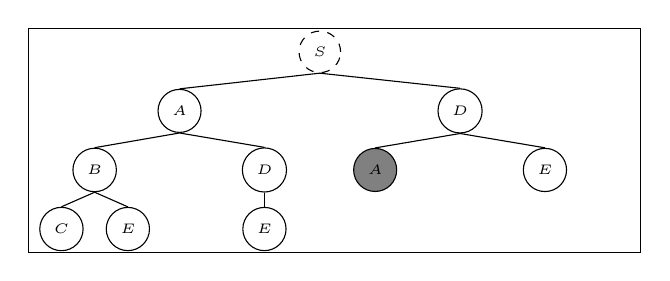
\begin{tikzpicture}[xscale=0.75,yscale=1,city/.style={shape=circle,draw=black},costc/.style={anchor=south east},heurh/.style={anchor=north east,gray},cityG/.style={city,very thick},cityM/.style={city,fill=gray}]
\def\dy{-0.75};
\def\dxa{4.75};
\def\dxb{2.875};
\def\dxc{1.125};
\def\dxd{0.75};
\def\dxe{0.75};

\draw (-0.5*\dxa-0.5*\dxb-\dxc,0.3) rectangle (0.5*\dxa+0.5*\dxb+\dxc+0.5,3*\dy-0.3);

\node[city,dashed] (S) at (0,0) {\tiny $S$};

\node[city] (A) at (-0.5*\dxa,\dy) {\tiny $A$};
\draw (S.south) -- (A.north);
\node[city] (D) at (0.5*\dxa,\dy) {\tiny $D$};
\draw (S.south) -- (D.north);

\node[city] (B) at (-0.5*\dxa-0.5*\dxb,2*\dy) {\tiny $B$};
\draw (A.south) -- (B.north);
\node[city] (D2) at (-0.5*\dxa+0.5*\dxb,2*\dy) {\tiny $D$};
\draw (A.south) -- (D2.north);
\node[cityM] (A2) at (0.5*\dxa-0.5*\dxb,2*\dy) {\tiny $A$};
\draw (D.south) -- (A2.north);
\node[city] (E) at (0.5*\dxa+0.5*\dxb,2*\dy) {\tiny $E$};
\draw (D.south) -- (E.north);

\node[city] (C) at (-0.5*\dxa-0.5*\dxb-0.5*\dxc,3*\dy) {\tiny $C$};
\draw (B.south) -- (C.north);
\node[city] (E2) at (-0.5*\dxa-0.5*\dxb+0.5*\dxc,3*\dy) {\tiny $E$};
\draw (B.south) -- (E2.north);
\node[city] (E3) at (-0.5*\dxa+0.5*\dxb,3*\dy) {\tiny $E$};
\draw (D2.south) -- (E3.north);
\end{tikzpicture}}
\subfigure{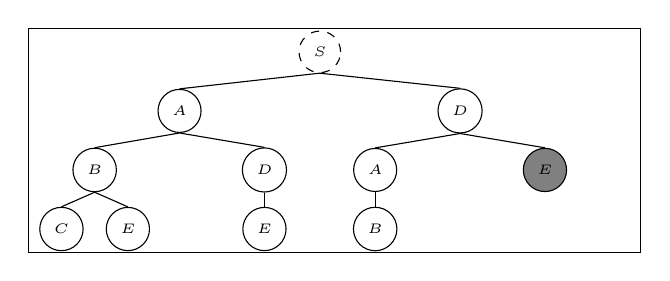
\begin{tikzpicture}[xscale=0.75,yscale=1,city/.style={shape=circle,draw=black},costc/.style={anchor=south east},heurh/.style={anchor=north east,gray},cityG/.style={city,very thick},cityM/.style={city,fill=gray}]
\def\dy{-0.75};
\def\dxa{4.75};
\def\dxb{2.875};
\def\dxc{1.125};
\def\dxd{0.75};
\def\dxe{0.75};

\draw (-0.5*\dxa-0.5*\dxb-\dxc,0.3) rectangle (0.5*\dxa+0.5*\dxb+\dxc+0.5,3*\dy-0.3);

\node[city,dashed] (S) at (0,0) {\tiny $S$};

\node[city] (A) at (-0.5*\dxa,\dy) {\tiny $A$};
\draw (S.south) -- (A.north);
\node[city] (D) at (0.5*\dxa,\dy) {\tiny $D$};
\draw (S.south) -- (D.north);

\node[city] (B) at (-0.5*\dxa-0.5*\dxb,2*\dy) {\tiny $B$};
\draw (A.south) -- (B.north);
\node[city] (D2) at (-0.5*\dxa+0.5*\dxb,2*\dy) {\tiny $D$};
\draw (A.south) -- (D2.north);
\node[city] (A2) at (0.5*\dxa-0.5*\dxb,2*\dy) {\tiny $A$};
\draw (D.south) -- (A2.north);
\node[cityM] (E) at (0.5*\dxa+0.5*\dxb,2*\dy) {\tiny $E$};
\draw (D.south) -- (E.north);

\node[city] (C) at (-0.5*\dxa-0.5*\dxb-0.5*\dxc,3*\dy) {\tiny $C$};
\draw (B.south) -- (C.north);
\node[city] (E2) at (-0.5*\dxa-0.5*\dxb+0.5*\dxc,3*\dy) {\tiny $E$};
\draw (B.south) -- (E2.north);
\node[city] (E3) at (-0.5*\dxa+0.5*\dxb,3*\dy) {\tiny $E$};
\draw (D2.south) -- (E3.north);
\node[city] (B2) at (0.5*\dxa-0.5*\dxb,3*\dy) {\tiny $B$};
\draw (A2.south) -- (B2.north);
\end{tikzpicture}}
\subfigure{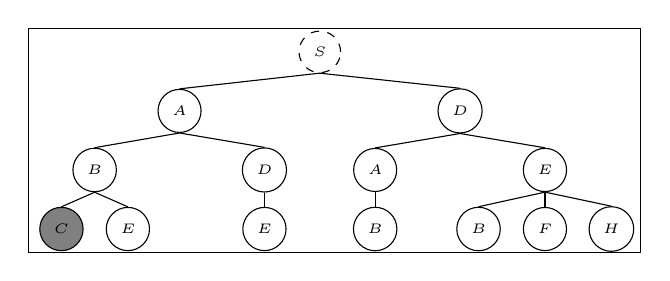
\begin{tikzpicture}[xscale=0.75,yscale=1,city/.style={shape=circle,draw=black},costc/.style={anchor=south east},heurh/.style={anchor=north east,gray},cityG/.style={city,very thick},cityM/.style={city,fill=gray}]
\def\dy{-0.75};
\def\dxa{4.75};
\def\dxb{2.875};
\def\dxc{1.125};
\def\dxd{0.75};
\def\dxe{0.75};

\draw (-0.5*\dxa-0.5*\dxb-\dxc,0.3) rectangle (0.5*\dxa+0.5*\dxb+\dxc+0.5,3*\dy-0.3);

\node[city,dashed] (S) at (0,0) {\tiny $S$};

\node[city] (A) at (-0.5*\dxa,\dy) {\tiny $A$};
\draw (S.south) -- (A.north);
\node[city] (D) at (0.5*\dxa,\dy) {\tiny $D$};
\draw (S.south) -- (D.north);

\node[city] (B) at (-0.5*\dxa-0.5*\dxb,2*\dy) {\tiny $B$};
\draw (A.south) -- (B.north);
\node[city] (D2) at (-0.5*\dxa+0.5*\dxb,2*\dy) {\tiny $D$};
\draw (A.south) -- (D2.north);
\node[city] (A2) at (0.5*\dxa-0.5*\dxb,2*\dy) {\tiny $A$};
\draw (D.south) -- (A2.north);
\node[city] (E) at (0.5*\dxa+0.5*\dxb,2*\dy) {\tiny $E$};
\draw (D.south) -- (E.north);

\node[cityM] (C) at (-0.5*\dxa-0.5*\dxb-0.5*\dxc,3*\dy) {\tiny $C$};
\draw (B.south) -- (C.north);
\node[city] (E2) at (-0.5*\dxa-0.5*\dxb+0.5*\dxc,3*\dy) {\tiny $E$};
\draw (B.south) -- (E2.north);
\node[city] (E3) at (-0.5*\dxa+0.5*\dxb,3*\dy) {\tiny $E$};
\draw (D2.south) -- (E3.north);
\node[city] (B2) at (0.5*\dxa-0.5*\dxb,3*\dy) {\tiny $B$};
\draw (A2.south) -- (B2.north);
\node[city] (B3) at (0.5*\dxa+0.5*\dxb-\dxc,3*\dy) {\tiny $B$};
\draw (E.south) -- (B3.north);
\node[city] (F) at (0.5*\dxa+0.5*\dxb,3*\dy) {\tiny $F$};
\draw (E.south) -- (F.north);
\node[city] (H) at (0.5*\dxa+0.5*\dxb+\dxc,3*\dy) {\tiny $H$};
\draw (E.south) -- (H.north);
\end{tikzpicture}}
\subfigure{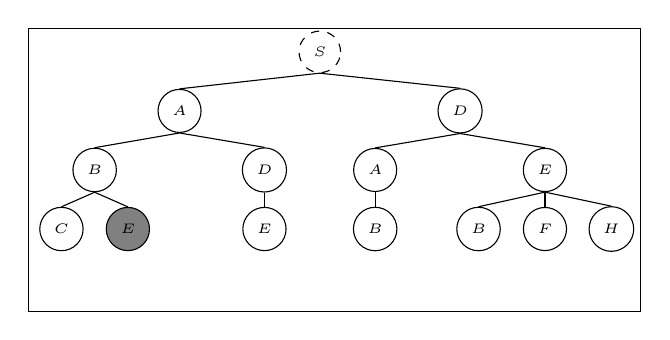
\begin{tikzpicture}[xscale=0.75,yscale=1,city/.style={shape=circle,draw=black},costc/.style={anchor=south east},heurh/.style={anchor=north east,gray},cityG/.style={city,very thick},cityM/.style={city,fill=gray}]
\def\dy{-0.75};
\def\dxa{4.75};
\def\dxb{2.875};
\def\dxc{1.125};
\def\dxd{0.75};
\def\dxe{0.75};

\draw (-0.5*\dxa-0.5*\dxb-\dxc,0.3) rectangle (0.5*\dxa+0.5*\dxb+\dxc+0.5,4*\dy-0.3);

\node[city,dashed] (S) at (0,0) {\tiny $S$};

\node[city] (A) at (-0.5*\dxa,\dy) {\tiny $A$};
\draw (S.south) -- (A.north);
\node[city] (D) at (0.5*\dxa,\dy) {\tiny $D$};
\draw (S.south) -- (D.north);

\node[city] (B) at (-0.5*\dxa-0.5*\dxb,2*\dy) {\tiny $B$};
\draw (A.south) -- (B.north);
\node[city] (D2) at (-0.5*\dxa+0.5*\dxb,2*\dy) {\tiny $D$};
\draw (A.south) -- (D2.north);
\node[city] (A2) at (0.5*\dxa-0.5*\dxb,2*\dy) {\tiny $A$};
\draw (D.south) -- (A2.north);
\node[city] (E) at (0.5*\dxa+0.5*\dxb,2*\dy) {\tiny $E$};
\draw (D.south) -- (E.north);

\node[city] (C) at (-0.5*\dxa-0.5*\dxb-0.5*\dxc,3*\dy) {\tiny $C$};
\draw (B.south) -- (C.north);
\node[cityM] (E2) at (-0.5*\dxa-0.5*\dxb+0.5*\dxc,3*\dy) {\tiny $E$};
\draw (B.south) -- (E2.north);
\node[city] (E3) at (-0.5*\dxa+0.5*\dxb,3*\dy) {\tiny $E$};
\draw (D2.south) -- (E3.north);
\node[city] (B2) at (0.5*\dxa-0.5*\dxb,3*\dy) {\tiny $B$};
\draw (A2.south) -- (B2.north);
\node[city] (B3) at (0.5*\dxa+0.5*\dxb-\dxc,3*\dy) {\tiny $B$};
\draw (E.south) -- (B3.north);
\node[city] (F) at (0.5*\dxa+0.5*\dxb,3*\dy) {\tiny $F$};
\draw (E.south) -- (F.north);
\node[city] (H) at (0.5*\dxa+0.5*\dxb+\dxc,3*\dy) {\tiny $H$};
\draw (E.south) -- (H.north);
\end{tikzpicture}}
\subfigure{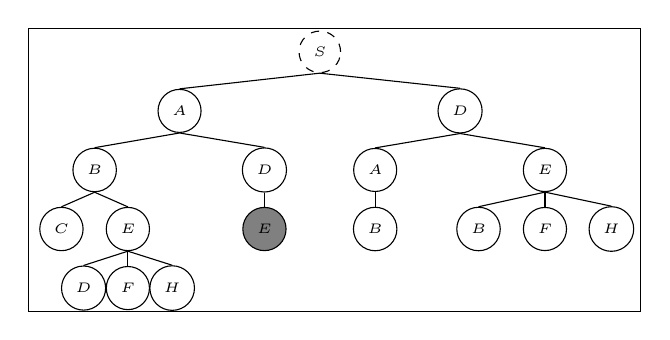
\begin{tikzpicture}[xscale=0.75,yscale=1,city/.style={shape=circle,draw=black},costc/.style={anchor=south east},heurh/.style={anchor=north east,gray},cityG/.style={city,very thick},cityM/.style={city,fill=gray}]
\def\dy{-0.75};
\def\dxa{4.75};
\def\dxb{2.875};
\def\dxc{1.125};
\def\dxd{0.75};
\def\dxe{0.75};

\draw (-0.5*\dxa-0.5*\dxb-\dxc,0.3) rectangle (0.5*\dxa+0.5*\dxb+\dxc+0.5,4*\dy-0.3);

\node[city,dashed] (S) at (0,0) {\tiny $S$};

\node[city] (A) at (-0.5*\dxa,\dy) {\tiny $A$};
\draw (S.south) -- (A.north);
\node[city] (D) at (0.5*\dxa,\dy) {\tiny $D$};
\draw (S.south) -- (D.north);

\node[city] (B) at (-0.5*\dxa-0.5*\dxb,2*\dy) {\tiny $B$};
\draw (A.south) -- (B.north);
\node[city] (D2) at (-0.5*\dxa+0.5*\dxb,2*\dy) {\tiny $D$};
\draw (A.south) -- (D2.north);
\node[city] (A2) at (0.5*\dxa-0.5*\dxb,2*\dy) {\tiny $A$};
\draw (D.south) -- (A2.north);
\node[city] (E) at (0.5*\dxa+0.5*\dxb,2*\dy) {\tiny $E$};
\draw (D.south) -- (E.north);

\node[city] (C) at (-0.5*\dxa-0.5*\dxb-0.5*\dxc,3*\dy) {\tiny $C$};
\draw (B.south) -- (C.north);
\node[city] (E2) at (-0.5*\dxa-0.5*\dxb+0.5*\dxc,3*\dy) {\tiny $E$};
\draw (B.south) -- (E2.north);
\node[cityM] (E3) at (-0.5*\dxa+0.5*\dxb,3*\dy) {\tiny $E$};
\draw (D2.south) -- (E3.north);
\node[city] (B2) at (0.5*\dxa-0.5*\dxb,3*\dy) {\tiny $B$};
\draw (A2.south) -- (B2.north);
\node[city] (B3) at (0.5*\dxa+0.5*\dxb-\dxc,3*\dy) {\tiny $B$};
\draw (E.south) -- (B3.north);
\node[city] (F) at (0.5*\dxa+0.5*\dxb,3*\dy) {\tiny $F$};
\draw (E.south) -- (F.north);
\node[city] (H) at (0.5*\dxa+0.5*\dxb+\dxc,3*\dy) {\tiny $H$};
\draw (E.south) -- (H.north);

\node[city] (D3) at (-0.5*\dxa-0.5*\dxb+0.5*\dxc-\dxd,4*\dy) {\tiny $D$};
\draw (E2.south) -- (D3.north);
\node[city] (F2) at (-0.5*\dxa-0.5*\dxb+0.5*\dxc,4*\dy) {\tiny $F$};
\draw (E2.south) -- (F2.north);
\node[city] (H2) at (-0.5*\dxa-0.5*\dxb+0.5*\dxc+\dxd,4*\dy) {\tiny $H$};
\draw (E2.south) -- (H2.north);
\end{tikzpicture}}
\subfigure{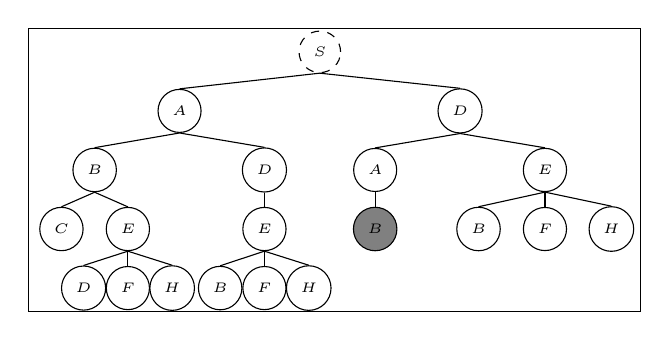
\begin{tikzpicture}[xscale=0.75,yscale=1,city/.style={shape=circle,draw=black},costc/.style={anchor=south east},heurh/.style={anchor=north east,gray},cityG/.style={city,very thick},cityM/.style={city,fill=gray}]
\def\dy{-0.75};
\def\dxa{4.75};
\def\dxb{2.875};
\def\dxc{1.125};
\def\dxd{0.75};
\def\dxe{0.75};

\draw (-0.5*\dxa-0.5*\dxb-\dxc,0.3) rectangle (0.5*\dxa+0.5*\dxb+\dxc+0.5,4*\dy-0.3);

\node[city,dashed] (S) at (0,0) {\tiny $S$};

\node[city] (A) at (-0.5*\dxa,\dy) {\tiny $A$};
\draw (S.south) -- (A.north);
\node[city] (D) at (0.5*\dxa,\dy) {\tiny $D$};
\draw (S.south) -- (D.north);

\node[city] (B) at (-0.5*\dxa-0.5*\dxb,2*\dy) {\tiny $B$};
\draw (A.south) -- (B.north);
\node[city] (D2) at (-0.5*\dxa+0.5*\dxb,2*\dy) {\tiny $D$};
\draw (A.south) -- (D2.north);
\node[city] (A2) at (0.5*\dxa-0.5*\dxb,2*\dy) {\tiny $A$};
\draw (D.south) -- (A2.north);
\node[city] (E) at (0.5*\dxa+0.5*\dxb,2*\dy) {\tiny $E$};
\draw (D.south) -- (E.north);

\node[city] (C) at (-0.5*\dxa-0.5*\dxb-0.5*\dxc,3*\dy) {\tiny $C$};
\draw (B.south) -- (C.north);
\node[city] (E2) at (-0.5*\dxa-0.5*\dxb+0.5*\dxc,3*\dy) {\tiny $E$};
\draw (B.south) -- (E2.north);
\node[city] (E3) at (-0.5*\dxa+0.5*\dxb,3*\dy) {\tiny $E$};
\draw (D2.south) -- (E3.north);
\node[cityM] (B2) at (0.5*\dxa-0.5*\dxb,3*\dy) {\tiny $B$};
\draw (A2.south) -- (B2.north);
\node[city] (B3) at (0.5*\dxa+0.5*\dxb-\dxc,3*\dy) {\tiny $B$};
\draw (E.south) -- (B3.north);
\node[city] (F) at (0.5*\dxa+0.5*\dxb,3*\dy) {\tiny $F$};
\draw (E.south) -- (F.north);
\node[city] (H) at (0.5*\dxa+0.5*\dxb+\dxc,3*\dy) {\tiny $H$};
\draw (E.south) -- (H.north);

\node[city] (D3) at (-0.5*\dxa-0.5*\dxb+0.5*\dxc-\dxd,4*\dy) {\tiny $D$};
\draw (E2.south) -- (D3.north);
\node[city] (F2) at (-0.5*\dxa-0.5*\dxb+0.5*\dxc,4*\dy) {\tiny $F$};
\draw (E2.south) -- (F2.north);
\node[city] (H2) at (-0.5*\dxa-0.5*\dxb+0.5*\dxc+\dxd,4*\dy) {\tiny $H$};
\draw (E2.south) -- (H2.north);
\node[city] (B4) at (-0.5*\dxa+0.5*\dxb-\dxd,4*\dy) {\tiny $B$};
\draw (E3.south) -- (B4.north);
\node[city] (F3) at (-0.5*\dxa+0.5*\dxb,4*\dy) {\tiny $F$};
\draw (E3.south) -- (F3.north);
\node[city] (H3) at (-0.5*\dxa+0.5*\dxb+\dxd,4*\dy) {\tiny $H$};
\draw (E3.south) -- (H3.north);
\end{tikzpicture}}
\subfigure{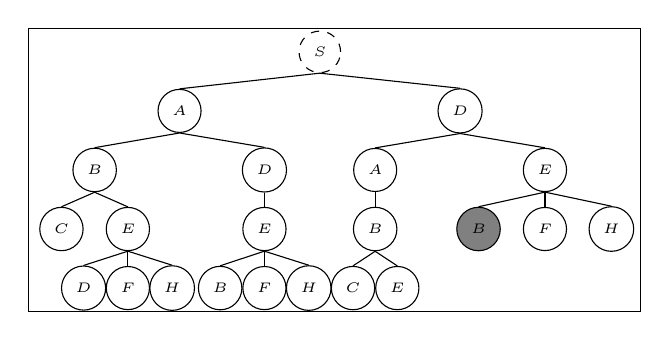
\begin{tikzpicture}[xscale=0.75,yscale=1,city/.style={shape=circle,draw=black},costc/.style={anchor=south east},heurh/.style={anchor=north east,gray},cityG/.style={city,very thick},cityM/.style={city,fill=gray}]
\def\dy{-0.75};
\def\dxa{4.75};
\def\dxb{2.875};
\def\dxc{1.125};
\def\dxd{0.75};
\def\dxe{0.75};

\draw (-0.5*\dxa-0.5*\dxb-\dxc,0.3) rectangle (0.5*\dxa+0.5*\dxb+\dxc+0.5,4*\dy-0.3);

\node[city,dashed] (S) at (0,0) {\tiny $S$};

\node[city] (A) at (-0.5*\dxa,\dy) {\tiny $A$};
\draw (S.south) -- (A.north);
\node[city] (D) at (0.5*\dxa,\dy) {\tiny $D$};
\draw (S.south) -- (D.north);

\node[city] (B) at (-0.5*\dxa-0.5*\dxb,2*\dy) {\tiny $B$};
\draw (A.south) -- (B.north);
\node[city] (D2) at (-0.5*\dxa+0.5*\dxb,2*\dy) {\tiny $D$};
\draw (A.south) -- (D2.north);
\node[city] (A2) at (0.5*\dxa-0.5*\dxb,2*\dy) {\tiny $A$};
\draw (D.south) -- (A2.north);
\node[city] (E) at (0.5*\dxa+0.5*\dxb,2*\dy) {\tiny $E$};
\draw (D.south) -- (E.north);

\node[city] (C) at (-0.5*\dxa-0.5*\dxb-0.5*\dxc,3*\dy) {\tiny $C$};
\draw (B.south) -- (C.north);
\node[city] (E2) at (-0.5*\dxa-0.5*\dxb+0.5*\dxc,3*\dy) {\tiny $E$};
\draw (B.south) -- (E2.north);
\node[city] (E3) at (-0.5*\dxa+0.5*\dxb,3*\dy) {\tiny $E$};
\draw (D2.south) -- (E3.north);
\node[city] (B2) at (0.5*\dxa-0.5*\dxb,3*\dy) {\tiny $B$};
\draw (A2.south) -- (B2.north);
\node[cityM] (B3) at (0.5*\dxa+0.5*\dxb-\dxc,3*\dy) {\tiny $B$};
\draw (E.south) -- (B3.north);
\node[city] (F) at (0.5*\dxa+0.5*\dxb,3*\dy) {\tiny $F$};
\draw (E.south) -- (F.north);
\node[city] (H) at (0.5*\dxa+0.5*\dxb+\dxc,3*\dy) {\tiny $H$};
\draw (E.south) -- (H.north);

\node[city] (D3) at (-0.5*\dxa-0.5*\dxb+0.5*\dxc-\dxd,4*\dy) {\tiny $D$};
\draw (E2.south) -- (D3.north);
\node[city] (F2) at (-0.5*\dxa-0.5*\dxb+0.5*\dxc,4*\dy) {\tiny $F$};
\draw (E2.south) -- (F2.north);
\node[city] (H2) at (-0.5*\dxa-0.5*\dxb+0.5*\dxc+\dxd,4*\dy) {\tiny $H$};
\draw (E2.south) -- (H2.north);
\node[city] (B4) at (-0.5*\dxa+0.5*\dxb-\dxd,4*\dy) {\tiny $B$};
\draw (E3.south) -- (B4.north);
\node[city] (F3) at (-0.5*\dxa+0.5*\dxb,4*\dy) {\tiny $F$};
\draw (E3.south) -- (F3.north);
\node[city] (H3) at (-0.5*\dxa+0.5*\dxb+\dxd,4*\dy) {\tiny $H$};
\draw (E3.south) -- (H3.north);
\node[city] (C2) at (0.5*\dxa-0.5*\dxb-0.5*\dxd,4*\dy) {\tiny $C$};
\draw (B2.south) -- (C2.north);
\node[city] (E4) at (0.5*\dxa-0.5*\dxb+0.5*\dxd,4*\dy) {\tiny $E$};
\draw (B2.south) -- (E4.north);
\end{tikzpicture}}
\subfigure{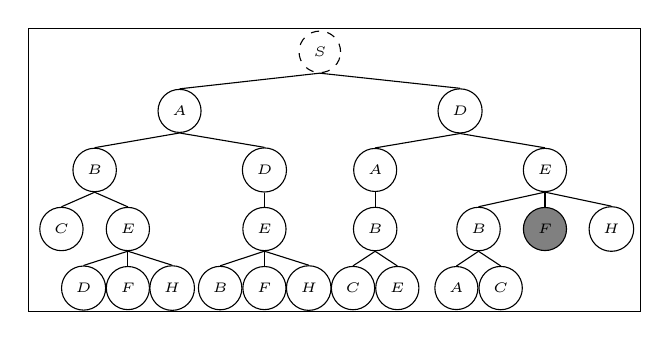
\begin{tikzpicture}[xscale=0.75,yscale=1,city/.style={shape=circle,draw=black},costc/.style={anchor=south east},heurh/.style={anchor=north east,gray},cityG/.style={city,very thick},cityM/.style={city,fill=gray}]
\def\dy{-0.75};
\def\dxa{4.75};
\def\dxb{2.875};
\def\dxc{1.125};
\def\dxd{0.75};
\def\dxe{0.75};

\draw (-0.5*\dxa-0.5*\dxb-\dxc,0.3) rectangle (0.5*\dxa+0.5*\dxb+\dxc+0.5,4*\dy-0.3);

\node[city,dashed] (S) at (0,0) {\tiny $S$};

\node[city] (A) at (-0.5*\dxa,\dy) {\tiny $A$};
\draw (S.south) -- (A.north);
\node[city] (D) at (0.5*\dxa,\dy) {\tiny $D$};
\draw (S.south) -- (D.north);

\node[city] (B) at (-0.5*\dxa-0.5*\dxb,2*\dy) {\tiny $B$};
\draw (A.south) -- (B.north);
\node[city] (D2) at (-0.5*\dxa+0.5*\dxb,2*\dy) {\tiny $D$};
\draw (A.south) -- (D2.north);
\node[city] (A2) at (0.5*\dxa-0.5*\dxb,2*\dy) {\tiny $A$};
\draw (D.south) -- (A2.north);
\node[city] (E) at (0.5*\dxa+0.5*\dxb,2*\dy) {\tiny $E$};
\draw (D.south) -- (E.north);

\node[city] (C) at (-0.5*\dxa-0.5*\dxb-0.5*\dxc,3*\dy) {\tiny $C$};
\draw (B.south) -- (C.north);
\node[city] (E2) at (-0.5*\dxa-0.5*\dxb+0.5*\dxc,3*\dy) {\tiny $E$};
\draw (B.south) -- (E2.north);
\node[city] (E3) at (-0.5*\dxa+0.5*\dxb,3*\dy) {\tiny $E$};
\draw (D2.south) -- (E3.north);
\node[city] (B2) at (0.5*\dxa-0.5*\dxb,3*\dy) {\tiny $B$};
\draw (A2.south) -- (B2.north);
\node[city] (B3) at (0.5*\dxa+0.5*\dxb-\dxc,3*\dy) {\tiny $B$};
\draw (E.south) -- (B3.north);
\node[cityM] (F) at (0.5*\dxa+0.5*\dxb,3*\dy) {\tiny $F$};
\draw (E.south) -- (F.north);
\node[city] (H) at (0.5*\dxa+0.5*\dxb+\dxc,3*\dy) {\tiny $H$};
\draw (E.south) -- (H.north);

\node[city] (D3) at (-0.5*\dxa-0.5*\dxb+0.5*\dxc-\dxd,4*\dy) {\tiny $D$};
\draw (E2.south) -- (D3.north);
\node[city] (F2) at (-0.5*\dxa-0.5*\dxb+0.5*\dxc,4*\dy) {\tiny $F$};
\draw (E2.south) -- (F2.north);
\node[city] (H2) at (-0.5*\dxa-0.5*\dxb+0.5*\dxc+\dxd,4*\dy) {\tiny $H$};
\draw (E2.south) -- (H2.north);
\node[city] (B4) at (-0.5*\dxa+0.5*\dxb-\dxd,4*\dy) {\tiny $B$};
\draw (E3.south) -- (B4.north);
\node[city] (F3) at (-0.5*\dxa+0.5*\dxb,4*\dy) {\tiny $F$};
\draw (E3.south) -- (F3.north);
\node[city] (H3) at (-0.5*\dxa+0.5*\dxb+\dxd,4*\dy) {\tiny $H$};
\draw (E3.south) -- (H3.north);
\node[city] (C2) at (0.5*\dxa-0.5*\dxb-0.5*\dxd,4*\dy) {\tiny $C$};
\draw (B2.south) -- (C2.north);
\node[city] (E4) at (0.5*\dxa-0.5*\dxb+0.5*\dxd,4*\dy) {\tiny $E$};
\draw (B2.south) -- (E4.north);
\node[city] (A3) at (0.5*\dxa+0.5*\dxb-\dxc-0.5*\dxd,4*\dy) {\tiny $A$};
\draw (B3.south) -- (A3.north);
\node[city] (C3) at (0.5*\dxa+0.5*\dxb-\dxc+0.5*\dxd,4*\dy) {\tiny $C$};
\draw (B3.south) -- (C3.north);
\end{tikzpicture}}
\subfigure{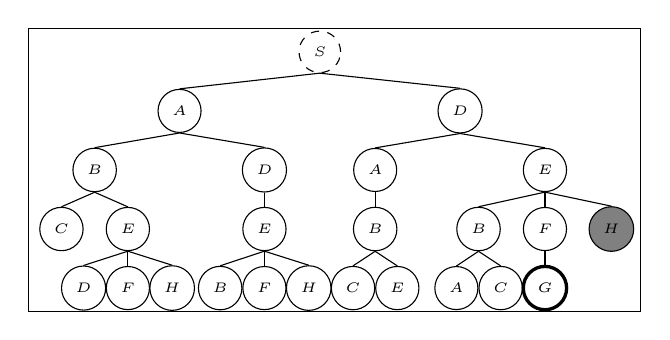
\begin{tikzpicture}[xscale=0.75,yscale=1,city/.style={shape=circle,draw=black},costc/.style={anchor=south east},heurh/.style={anchor=north east,gray},cityG/.style={city,very thick},cityM/.style={city,fill=gray}]
\def\dy{-0.75};
\def\dxa{4.75};
\def\dxb{2.875};
\def\dxc{1.125};
\def\dxd{0.75};
\def\dxe{0.75};

\draw (-0.5*\dxa-0.5*\dxb-\dxc,0.3) rectangle (0.5*\dxa+0.5*\dxb+\dxc+0.5,4*\dy-0.3);

\node[city,dashed] (S) at (0,0) {\tiny $S$};

\node[city] (A) at (-0.5*\dxa,\dy) {\tiny $A$};
\draw (S.south) -- (A.north);
\node[city] (D) at (0.5*\dxa,\dy) {\tiny $D$};
\draw (S.south) -- (D.north);

\node[city] (B) at (-0.5*\dxa-0.5*\dxb,2*\dy) {\tiny $B$};
\draw (A.south) -- (B.north);
\node[city] (D2) at (-0.5*\dxa+0.5*\dxb,2*\dy) {\tiny $D$};
\draw (A.south) -- (D2.north);
\node[city] (A2) at (0.5*\dxa-0.5*\dxb,2*\dy) {\tiny $A$};
\draw (D.south) -- (A2.north);
\node[city] (E) at (0.5*\dxa+0.5*\dxb,2*\dy) {\tiny $E$};
\draw (D.south) -- (E.north);

\node[city] (C) at (-0.5*\dxa-0.5*\dxb-0.5*\dxc,3*\dy) {\tiny $C$};
\draw (B.south) -- (C.north);
\node[city] (E2) at (-0.5*\dxa-0.5*\dxb+0.5*\dxc,3*\dy) {\tiny $E$};
\draw (B.south) -- (E2.north);
\node[city] (E3) at (-0.5*\dxa+0.5*\dxb,3*\dy) {\tiny $E$};
\draw (D2.south) -- (E3.north);
\node[city] (B2) at (0.5*\dxa-0.5*\dxb,3*\dy) {\tiny $B$};
\draw (A2.south) -- (B2.north);
\node[city] (B3) at (0.5*\dxa+0.5*\dxb-\dxc,3*\dy) {\tiny $B$};
\draw (E.south) -- (B3.north);
\node[city] (F) at (0.5*\dxa+0.5*\dxb,3*\dy) {\tiny $F$};
\draw (E.south) -- (F.north);
\node[cityM] (H) at (0.5*\dxa+0.5*\dxb+\dxc,3*\dy) {\tiny $H$};
\draw (E.south) -- (H.north);

\node[city] (D3) at (-0.5*\dxa-0.5*\dxb+0.5*\dxc-\dxd,4*\dy) {\tiny $D$};
\draw (E2.south) -- (D3.north);
\node[city] (F2) at (-0.5*\dxa-0.5*\dxb+0.5*\dxc,4*\dy) {\tiny $F$};
\draw (E2.south) -- (F2.north);
\node[city] (H2) at (-0.5*\dxa-0.5*\dxb+0.5*\dxc+\dxd,4*\dy) {\tiny $H$};
\draw (E2.south) -- (H2.north);
\node[city] (B4) at (-0.5*\dxa+0.5*\dxb-\dxd,4*\dy) {\tiny $B$};
\draw (E3.south) -- (B4.north);
\node[city] (F3) at (-0.5*\dxa+0.5*\dxb,4*\dy) {\tiny $F$};
\draw (E3.south) -- (F3.north);
\node[city] (H3) at (-0.5*\dxa+0.5*\dxb+\dxd,4*\dy) {\tiny $H$};
\draw (E3.south) -- (H3.north);
\node[city] (C2) at (0.5*\dxa-0.5*\dxb-0.5*\dxd,4*\dy) {\tiny $C$};
\draw (B2.south) -- (C2.north);
\node[city] (E4) at (0.5*\dxa-0.5*\dxb+0.5*\dxd,4*\dy) {\tiny $E$};
\draw (B2.south) -- (E4.north);
\node[city] (A3) at (0.5*\dxa+0.5*\dxb-\dxc-0.5*\dxd,4*\dy) {\tiny $A$};
\draw (B3.south) -- (A3.north);
\node[city] (C3) at (0.5*\dxa+0.5*\dxb-\dxc+0.5*\dxd,4*\dy) {\tiny $C$};
\draw (B3.south) -- (C3.north);
\node[cityG] (G) at (0.5*\dxa+0.5*\dxb,4*\dy) {\tiny $G$};
\draw (F.south) -- (G.north);
\end{tikzpicture}}
\caption{Breadth-First toegepast op het wegenplan}
\label{fig:breadthFirstCity}
\end{figure}
\begin{figure}[H]
\centering
\subfigure{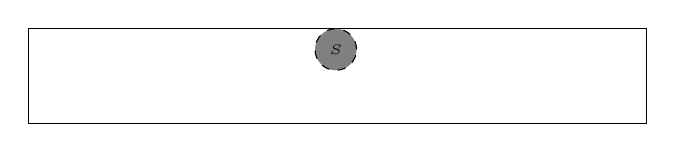
\begin{tikzpicture}[xscale=0.725,yscale=0.9,city/.style={shape=circle,draw=black},cityG/.style={city,very thick},cityM/.style={city,fill=gray}]
\def\dy{-0.75};
\def\dxa{4.75};
\def\dxb{2.875};
\def\dxc{1.125};
\def\dxd{0.75};
\def\dxe{0.75};

\draw (-0.5*\dxa-0.5*\dxb-\dxc-0.45,0.3) rectangle (0.5*\dxa+0.5*\dxb+\dxc+0.5,1*\dy-0.3);

\node[cityM,dashed] (S) at (0,0) {\tiny $S$};

\end{tikzpicture}}
\subfigure{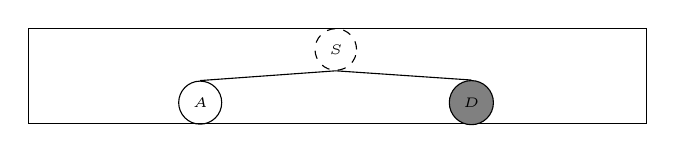
\begin{tikzpicture}[xscale=0.725,yscale=0.9,city/.style={shape=circle,draw=black},cityG/.style={city,very thick},cityM/.style={city,fill=gray}]
\def\dy{-0.75};
\def\dxa{4.75};
\def\dxb{2.875};
\def\dxc{1.125};
\def\dxd{0.75};
\def\dxe{0.75};

\draw (-0.5*\dxa-0.5*\dxb-\dxc-0.45,0.3) rectangle (0.5*\dxa+0.5*\dxb+\dxc+0.5,1*\dy-0.3);

\node[city,dashed] (S) at (0,0) {\tiny $S$};

\node[city] (A) at (-0.5*\dxa,\dy) {\tiny $A$};
\draw (S.south) -- (A.north);
\node[cityM] (D) at (0.5*\dxa,\dy) {\tiny $D$};
\draw (S.south) -- (D.north);

\end{tikzpicture}}
\subfigure{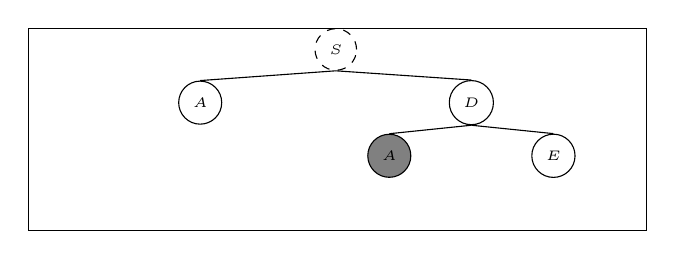
\begin{tikzpicture}[xscale=0.725,yscale=0.9,city/.style={shape=circle,draw=black},cityG/.style={city,very thick},cityM/.style={city,fill=gray}]
\def\dy{-0.75};
\def\dxa{4.75};
\def\dxb{2.875};
\def\dxc{1.125};
\def\dxd{0.75};
\def\dxe{0.75};

\draw (-0.5*\dxa-0.5*\dxb-\dxc-0.45,0.3) rectangle (0.5*\dxa+0.5*\dxb+\dxc+0.5,3*\dy-0.3);

\node[city,dashed] (S) at (0,0) {\tiny $S$};

\node[city] (A) at (-0.5*\dxa,\dy) {\tiny $A$};
\draw (S.south) -- (A.north);
\node[city] (D) at (0.5*\dxa,\dy) {\tiny $D$};
\draw (S.south) -- (D.north);

\node[cityM] (A2) at (0.5*\dxa-0.5*\dxb,2*\dy) {\tiny $A$};
\draw (D.south) -- (A2.north);
\node[city] (E) at (0.5*\dxa+0.5*\dxb,2*\dy) {\tiny $E$};
\draw (D.south) -- (E.north);
\end{tikzpicture}}
\subfigure{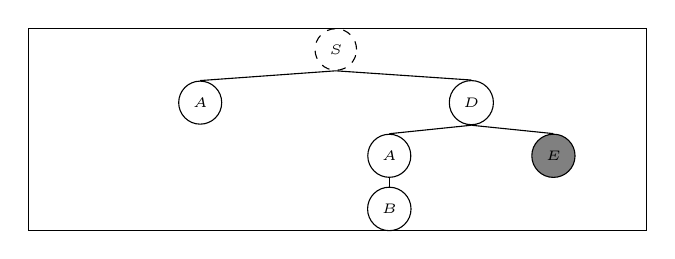
\begin{tikzpicture}[xscale=0.725,yscale=0.9,city/.style={shape=circle,draw=black},cityG/.style={city,very thick},cityM/.style={city,fill=gray}]
\def\dy{-0.75};
\def\dxa{4.75};
\def\dxb{2.875};
\def\dxc{1.125};
\def\dxd{0.75};
\def\dxe{0.75};

\draw (-0.5*\dxa-0.5*\dxb-\dxc-0.45,0.3) rectangle (0.5*\dxa+0.5*\dxb+\dxc+0.5,3*\dy-0.3);

\node[city,dashed] (S) at (0,0) {\tiny $S$};

\node[city] (A) at (-0.5*\dxa,\dy) {\tiny $A$};
\draw (S.south) -- (A.north);
\node[city] (D) at (0.5*\dxa,\dy) {\tiny $D$};
\draw (S.south) -- (D.north);

\node[city] (A2) at (0.5*\dxa-0.5*\dxb,2*\dy) {\tiny $A$};
\draw (D.south) -- (A2.north);
\node[cityM] (E) at (0.5*\dxa+0.5*\dxb,2*\dy) {\tiny $E$};
\draw (D.south) -- (E.north);

\node[city] (B2) at (0.5*\dxa-0.5*\dxb,3*\dy) {\tiny $B$};
\draw (A2.south) -- (B2.north);
\end{tikzpicture}}
\subfigure{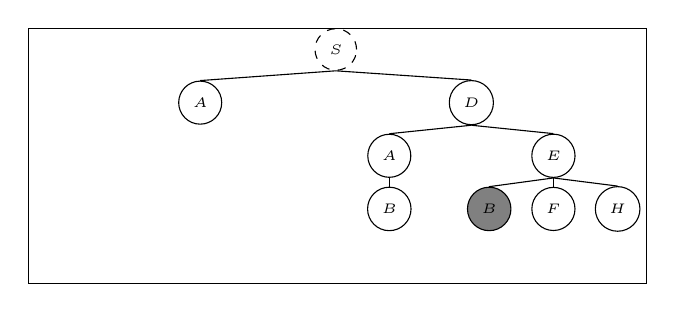
\begin{tikzpicture}[xscale=0.725,yscale=0.9,city/.style={shape=circle,draw=black},cityG/.style={city,very thick},cityM/.style={city,fill=gray}]
\def\dy{-0.75};
\def\dxa{4.75};
\def\dxb{2.875};
\def\dxc{1.125};
\def\dxd{0.75};
\def\dxe{0.75};

\draw (-0.5*\dxa-0.5*\dxb-\dxc-0.45,0.3) rectangle (0.5*\dxa+0.5*\dxb+\dxc+0.5,4*\dy-0.3);

\node[city,dashed] (S) at (0,0) {\tiny $S$};

\node[city] (A) at (-0.5*\dxa,\dy) {\tiny $A$};
\draw (S.south) -- (A.north);
\node[city] (D) at (0.5*\dxa,\dy) {\tiny $D$};
\draw (S.south) -- (D.north);

\node[city] (A2) at (0.5*\dxa-0.5*\dxb,2*\dy) {\tiny $A$};
\draw (D.south) -- (A2.north);
\node[city] (E) at (0.5*\dxa+0.5*\dxb,2*\dy) {\tiny $E$};
\draw (D.south) -- (E.north);

\node[city] (B2) at (0.5*\dxa-0.5*\dxb,3*\dy) {\tiny $B$};
\draw (A2.south) -- (B2.north);
\node[cityM] (B3) at (0.5*\dxa+0.5*\dxb-\dxc,3*\dy) {\tiny $B$};
\draw (E.south) -- (B3.north);
\node[city] (F) at (0.5*\dxa+0.5*\dxb,3*\dy) {\tiny $F$};
\draw (E.south) -- (F.north);
\node[city] (H) at (0.5*\dxa+0.5*\dxb+\dxc,3*\dy) {\tiny $H$};
\draw (E.south) -- (H.north);
\end{tikzpicture}}
\subfigure{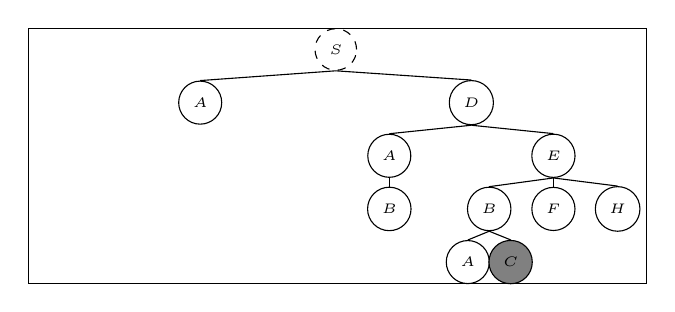
\begin{tikzpicture}[xscale=0.725,yscale=0.9,city/.style={shape=circle,draw=black},cityG/.style={city,very thick},cityM/.style={city,fill=gray}]
\def\dy{-0.75};
\def\dxa{4.75};
\def\dxb{2.875};
\def\dxc{1.125};
\def\dxd{0.75};
\def\dxe{0.75};

\draw (-0.5*\dxa-0.5*\dxb-\dxc-0.45,0.3) rectangle (0.5*\dxa+0.5*\dxb+\dxc+0.5,4*\dy-0.3);

\node[city,dashed] (S) at (0,0) {\tiny $S$};

\node[city] (A) at (-0.5*\dxa,\dy) {\tiny $A$};
\draw (S.south) -- (A.north);
\node[city] (D) at (0.5*\dxa,\dy) {\tiny $D$};
\draw (S.south) -- (D.north);

\node[city] (A2) at (0.5*\dxa-0.5*\dxb,2*\dy) {\tiny $A$};
\draw (D.south) -- (A2.north);
\node[city] (E) at (0.5*\dxa+0.5*\dxb,2*\dy) {\tiny $E$};
\draw (D.south) -- (E.north);

\node[city] (B2) at (0.5*\dxa-0.5*\dxb,3*\dy) {\tiny $B$};
\draw (A2.south) -- (B2.north);
\node[city] (B3) at (0.5*\dxa+0.5*\dxb-\dxc,3*\dy) {\tiny $B$};
\draw (E.south) -- (B3.north);
\node[city] (F) at (0.5*\dxa+0.5*\dxb,3*\dy) {\tiny $F$};
\draw (E.south) -- (F.north);
\node[city] (H) at (0.5*\dxa+0.5*\dxb+\dxc,3*\dy) {\tiny $H$};
\draw (E.south) -- (H.north);

\node[city] (A3) at (0.5*\dxa+0.5*\dxb-\dxc-0.5*\dxd,4*\dy) {\tiny $A$};
\draw (B3.south) -- (A3.north);
\node[cityM] (C3) at (0.5*\dxa+0.5*\dxb-\dxc+0.5*\dxd,4*\dy) {\tiny $C$};
\draw (B3.south) -- (C3.north);
\end{tikzpicture}}
\subfigure{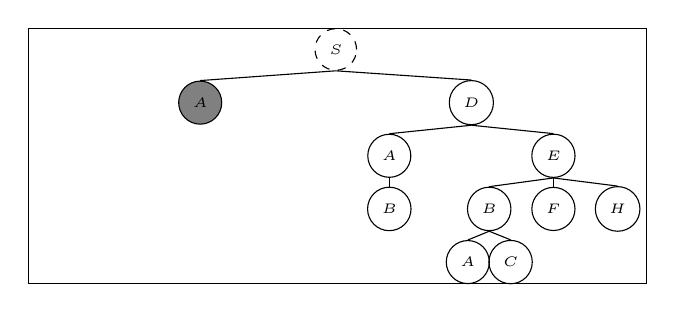
\begin{tikzpicture}[xscale=0.725,yscale=0.9,city/.style={shape=circle,draw=black},cityG/.style={city,very thick},cityM/.style={city,fill=gray}]
\def\dy{-0.75};
\def\dxa{4.75};
\def\dxb{2.875};
\def\dxc{1.125};
\def\dxd{0.75};
\def\dxe{0.75};

\draw (-0.5*\dxa-0.5*\dxb-\dxc-0.45,0.3) rectangle (0.5*\dxa+0.5*\dxb+\dxc+0.5,4*\dy-0.3);

\node[city,dashed] (S) at (0,0) {\tiny $S$};

\node[cityM] (A) at (-0.5*\dxa,\dy) {\tiny $A$};
\draw (S.south) -- (A.north);
\node[city] (D) at (0.5*\dxa,\dy) {\tiny $D$};
\draw (S.south) -- (D.north);

\node[city] (A2) at (0.5*\dxa-0.5*\dxb,2*\dy) {\tiny $A$};
\draw (D.south) -- (A2.north);
\node[city] (E) at (0.5*\dxa+0.5*\dxb,2*\dy) {\tiny $E$};
\draw (D.south) -- (E.north);

\node[city] (B2) at (0.5*\dxa-0.5*\dxb,3*\dy) {\tiny $B$};
\draw (A2.south) -- (B2.north);
\node[city] (B3) at (0.5*\dxa+0.5*\dxb-\dxc,3*\dy) {\tiny $B$};
\draw (E.south) -- (B3.north);
\node[city] (F) at (0.5*\dxa+0.5*\dxb,3*\dy) {\tiny $F$};
\draw (E.south) -- (F.north);
\node[city] (H) at (0.5*\dxa+0.5*\dxb+\dxc,3*\dy) {\tiny $H$};
\draw (E.south) -- (H.north);

\node[city] (A3) at (0.5*\dxa+0.5*\dxb-\dxc-0.5*\dxd,4*\dy) {\tiny $A$};
\draw (B3.south) -- (A3.north);
\node[city] (C3) at (0.5*\dxa+0.5*\dxb-\dxc+0.5*\dxd,4*\dy) {\tiny $C$};
\draw (B3.south) -- (C3.north);
\end{tikzpicture}}
\subfigure{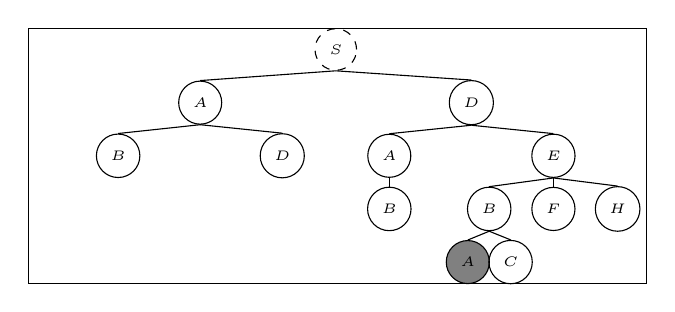
\begin{tikzpicture}[xscale=0.725,yscale=0.9,city/.style={shape=circle,draw=black},cityG/.style={city,very thick},cityM/.style={city,fill=gray}]
\def\dy{-0.75};
\def\dxa{4.75};
\def\dxb{2.875};
\def\dxc{1.125};
\def\dxd{0.75};
\def\dxe{0.75};

\draw (-0.5*\dxa-0.5*\dxb-\dxc-0.45,0.3) rectangle (0.5*\dxa+0.5*\dxb+\dxc+0.5,4*\dy-0.3);

\node[city,dashed] (S) at (0,0) {\tiny $S$};

\node[city] (A) at (-0.5*\dxa,\dy) {\tiny $A$};
\draw (S.south) -- (A.north);
\node[city] (D) at (0.5*\dxa,\dy) {\tiny $D$};
\draw (S.south) -- (D.north);

\node[city] (B) at (-0.5*\dxa-0.5*\dxb,2*\dy) {\tiny $B$};
\draw (A.south) -- (B.north);
\node[city] (D2) at (-0.5*\dxa+0.5*\dxb,2*\dy) {\tiny $D$};
\draw (A.south) -- (D2.north);
\node[city] (A2) at (0.5*\dxa-0.5*\dxb,2*\dy) {\tiny $A$};
\draw (D.south) -- (A2.north);
\node[city] (E) at (0.5*\dxa+0.5*\dxb,2*\dy) {\tiny $E$};
\draw (D.south) -- (E.north);

\node[city] (B2) at (0.5*\dxa-0.5*\dxb,3*\dy) {\tiny $B$};
\draw (A2.south) -- (B2.north);
\node[city] (B3) at (0.5*\dxa+0.5*\dxb-\dxc,3*\dy) {\tiny $B$};
\draw (E.south) -- (B3.north);
\node[city] (F) at (0.5*\dxa+0.5*\dxb,3*\dy) {\tiny $F$};
\draw (E.south) -- (F.north);
\node[city] (H) at (0.5*\dxa+0.5*\dxb+\dxc,3*\dy) {\tiny $H$};
\draw (E.south) -- (H.north);

\node[cityM] (A3) at (0.5*\dxa+0.5*\dxb-\dxc-0.5*\dxd,4*\dy) {\tiny $A$};
\draw (B3.south) -- (A3.north);
\node[city] (C3) at (0.5*\dxa+0.5*\dxb-\dxc+0.5*\dxd,4*\dy) {\tiny $C$};
\draw (B3.south) -- (C3.north);
\end{tikzpicture}}
\subfigure{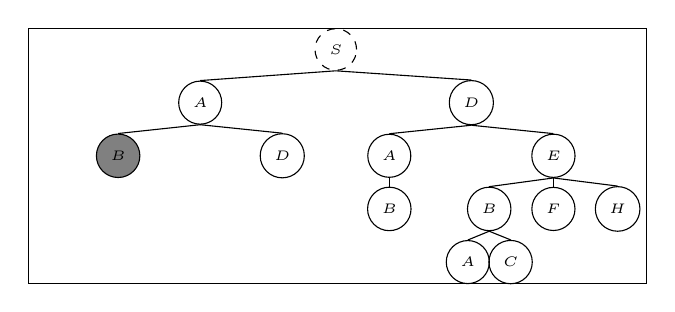
\begin{tikzpicture}[xscale=0.725,yscale=0.9,city/.style={shape=circle,draw=black},cityG/.style={city,very thick},cityM/.style={city,fill=gray}]
\def\dy{-0.75};
\def\dxa{4.75};
\def\dxb{2.875};
\def\dxc{1.125};
\def\dxd{0.75};
\def\dxe{0.75};

\draw (-0.5*\dxa-0.5*\dxb-\dxc-0.45,0.3) rectangle (0.5*\dxa+0.5*\dxb+\dxc+0.5,4*\dy-0.3);

\node[city,dashed] (S) at (0,0) {\tiny $S$};

\node[city] (A) at (-0.5*\dxa,\dy) {\tiny $A$};
\draw (S.south) -- (A.north);
\node[city] (D) at (0.5*\dxa,\dy) {\tiny $D$};
\draw (S.south) -- (D.north);

\node[cityM] (B) at (-0.5*\dxa-0.5*\dxb,2*\dy) {\tiny $B$};
\draw (A.south) -- (B.north);
\node[city] (D2) at (-0.5*\dxa+0.5*\dxb,2*\dy) {\tiny $D$};
\draw (A.south) -- (D2.north);
\node[city] (A2) at (0.5*\dxa-0.5*\dxb,2*\dy) {\tiny $A$};
\draw (D.south) -- (A2.north);
\node[city] (E) at (0.5*\dxa+0.5*\dxb,2*\dy) {\tiny $E$};
\draw (D.south) -- (E.north);

\node[city] (B2) at (0.5*\dxa-0.5*\dxb,3*\dy) {\tiny $B$};
\draw (A2.south) -- (B2.north);
\node[city] (B3) at (0.5*\dxa+0.5*\dxb-\dxc,3*\dy) {\tiny $B$};
\draw (E.south) -- (B3.north);
\node[city] (F) at (0.5*\dxa+0.5*\dxb,3*\dy) {\tiny $F$};
\draw (E.south) -- (F.north);
\node[city] (H) at (0.5*\dxa+0.5*\dxb+\dxc,3*\dy) {\tiny $H$};
\draw (E.south) -- (H.north);

\node[city] (A3) at (0.5*\dxa+0.5*\dxb-\dxc-0.5*\dxd,4*\dy) {\tiny $A$};
\draw (B3.south) -- (A3.north);
\node[city] (C3) at (0.5*\dxa+0.5*\dxb-\dxc+0.5*\dxd,4*\dy) {\tiny $C$};
\draw (B3.south) -- (C3.north);
\end{tikzpicture}}
\subfigure{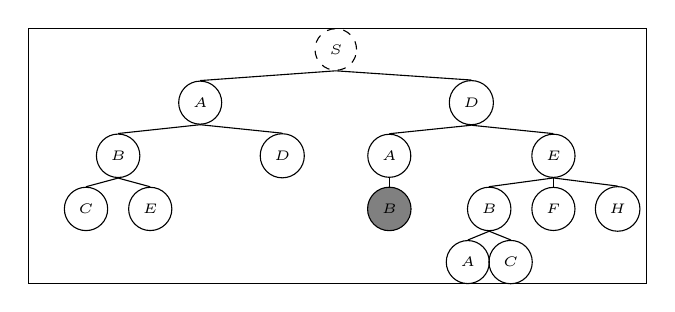
\begin{tikzpicture}[xscale=0.725,yscale=0.9,city/.style={shape=circle,draw=black},cityG/.style={city,very thick},cityM/.style={city,fill=gray}]
\def\dy{-0.75};
\def\dxa{4.75};
\def\dxb{2.875};
\def\dxc{1.125};
\def\dxd{0.75};
\def\dxe{0.75};

\draw (-0.5*\dxa-0.5*\dxb-\dxc-0.45,0.3) rectangle (0.5*\dxa+0.5*\dxb+\dxc+0.5,4*\dy-0.3);

\node[city,dashed] (S) at (0,0) {\tiny $S$};

\node[city] (A) at (-0.5*\dxa,\dy) {\tiny $A$};
\draw (S.south) -- (A.north);
\node[city] (D) at (0.5*\dxa,\dy) {\tiny $D$};
\draw (S.south) -- (D.north);

\node[city] (B) at (-0.5*\dxa-0.5*\dxb,2*\dy) {\tiny $B$};
\draw (A.south) -- (B.north);
\node[city] (D2) at (-0.5*\dxa+0.5*\dxb,2*\dy) {\tiny $D$};
\draw (A.south) -- (D2.north);
\node[city] (A2) at (0.5*\dxa-0.5*\dxb,2*\dy) {\tiny $A$};
\draw (D.south) -- (A2.north);
\node[city] (E) at (0.5*\dxa+0.5*\dxb,2*\dy) {\tiny $E$};
\draw (D.south) -- (E.north);

\node[city] (C) at (-0.5*\dxa-0.5*\dxb-0.5*\dxc,3*\dy) {\tiny $C$};
\draw (B.south) -- (C.north);
\node[city] (E2) at (-0.5*\dxa-0.5*\dxb+0.5*\dxc,3*\dy) {\tiny $E$};
\draw (B.south) -- (E2.north);
\node[cityM] (B2) at (0.5*\dxa-0.5*\dxb,3*\dy) {\tiny $B$};
\draw (A2.south) -- (B2.north);
\node[city] (B3) at (0.5*\dxa+0.5*\dxb-\dxc,3*\dy) {\tiny $B$};
\draw (E.south) -- (B3.north);
\node[city] (F) at (0.5*\dxa+0.5*\dxb,3*\dy) {\tiny $F$};
\draw (E.south) -- (F.north);
\node[city] (H) at (0.5*\dxa+0.5*\dxb+\dxc,3*\dy) {\tiny $H$};
\draw (E.south) -- (H.north);

\node[city] (A3) at (0.5*\dxa+0.5*\dxb-\dxc-0.5*\dxd,4*\dy) {\tiny $A$};
\draw (B3.south) -- (A3.north);
\node[city] (C3) at (0.5*\dxa+0.5*\dxb-\dxc+0.5*\dxd,4*\dy) {\tiny $C$};
\draw (B3.south) -- (C3.north);
\end{tikzpicture}}
\subfigure{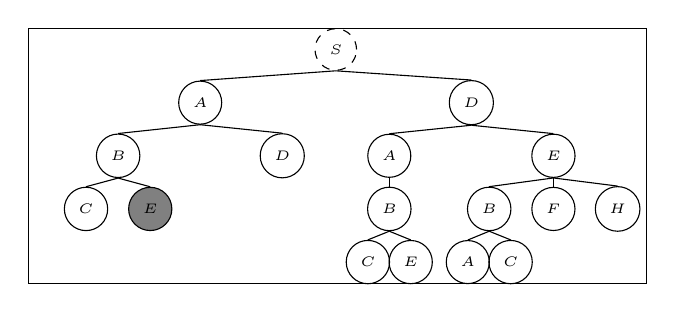
\begin{tikzpicture}[xscale=0.725,yscale=0.9,city/.style={shape=circle,draw=black},cityG/.style={city,very thick},cityM/.style={city,fill=gray}]
\def\dy{-0.75};
\def\dxa{4.75};
\def\dxb{2.875};
\def\dxc{1.125};
\def\dxd{0.75};
\def\dxe{0.75};

\draw (-0.5*\dxa-0.5*\dxb-\dxc-0.45,0.3) rectangle (0.5*\dxa+0.5*\dxb+\dxc+0.5,4*\dy-0.3);

\node[city,dashed] (S) at (0,0) {\tiny $S$};

\node[city] (A) at (-0.5*\dxa,\dy) {\tiny $A$};
\draw (S.south) -- (A.north);
\node[city] (D) at (0.5*\dxa,\dy) {\tiny $D$};
\draw (S.south) -- (D.north);

\node[city] (B) at (-0.5*\dxa-0.5*\dxb,2*\dy) {\tiny $B$};
\draw (A.south) -- (B.north);
\node[city] (D2) at (-0.5*\dxa+0.5*\dxb,2*\dy) {\tiny $D$};
\draw (A.south) -- (D2.north);
\node[city] (A2) at (0.5*\dxa-0.5*\dxb,2*\dy) {\tiny $A$};
\draw (D.south) -- (A2.north);
\node[city] (E) at (0.5*\dxa+0.5*\dxb,2*\dy) {\tiny $E$};
\draw (D.south) -- (E.north);

\node[city] (C) at (-0.5*\dxa-0.5*\dxb-0.5*\dxc,3*\dy) {\tiny $C$};
\draw (B.south) -- (C.north);
\node[cityM] (E2) at (-0.5*\dxa-0.5*\dxb+0.5*\dxc,3*\dy) {\tiny $E$};
\draw (B.south) -- (E2.north);
\node[city] (B2) at (0.5*\dxa-0.5*\dxb,3*\dy) {\tiny $B$};
\draw (A2.south) -- (B2.north);
\node[city] (B3) at (0.5*\dxa+0.5*\dxb-\dxc,3*\dy) {\tiny $B$};
\draw (E.south) -- (B3.north);
\node[city] (F) at (0.5*\dxa+0.5*\dxb,3*\dy) {\tiny $F$};
\draw (E.south) -- (F.north);
\node[city] (H) at (0.5*\dxa+0.5*\dxb+\dxc,3*\dy) {\tiny $H$};
\draw (E.south) -- (H.north);

\node[city] (C2) at (0.5*\dxa-0.5*\dxb-0.5*\dxd,4*\dy) {\tiny $C$};
\draw (B2.south) -- (C2.north);
\node[city] (E4) at (0.5*\dxa-0.5*\dxb+0.5*\dxd,4*\dy) {\tiny $E$};
\draw (B2.south) -- (E4.north);
\node[city] (A3) at (0.5*\dxa+0.5*\dxb-\dxc-0.5*\dxd,4*\dy) {\tiny $A$};
\draw (B3.south) -- (A3.north);
\node[city] (C3) at (0.5*\dxa+0.5*\dxb-\dxc+0.5*\dxd,4*\dy) {\tiny $C$};
\draw (B3.south) -- (C3.north);
\end{tikzpicture}}
\subfigure{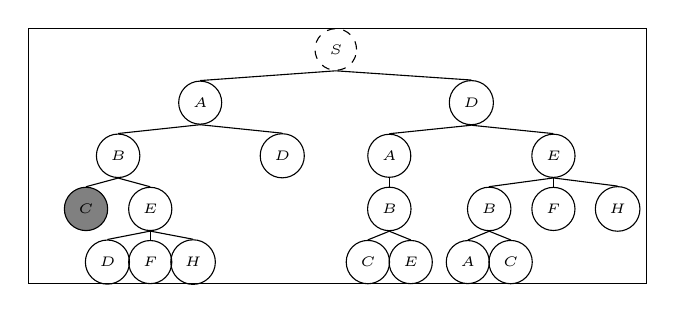
\begin{tikzpicture}[xscale=0.725,yscale=0.9,city/.style={shape=circle,draw=black},cityG/.style={city,very thick},cityM/.style={city,fill=gray}]
\def\dy{-0.75};
\def\dxa{4.75};
\def\dxb{2.875};
\def\dxc{1.125};
\def\dxd{0.75};
\def\dxe{0.75};

\draw (-0.5*\dxa-0.5*\dxb-\dxc-0.45,0.3) rectangle (0.5*\dxa+0.5*\dxb+\dxc+0.5,4*\dy-0.3);

\node[city,dashed] (S) at (0,0) {\tiny $S$};

\node[city] (A) at (-0.5*\dxa,\dy) {\tiny $A$};
\draw (S.south) -- (A.north);
\node[city] (D) at (0.5*\dxa,\dy) {\tiny $D$};
\draw (S.south) -- (D.north);

\node[city] (B) at (-0.5*\dxa-0.5*\dxb,2*\dy) {\tiny $B$};
\draw (A.south) -- (B.north);
\node[city] (D2) at (-0.5*\dxa+0.5*\dxb,2*\dy) {\tiny $D$};
\draw (A.south) -- (D2.north);
\node[city] (A2) at (0.5*\dxa-0.5*\dxb,2*\dy) {\tiny $A$};
\draw (D.south) -- (A2.north);
\node[city] (E) at (0.5*\dxa+0.5*\dxb,2*\dy) {\tiny $E$};
\draw (D.south) -- (E.north);

\node[cityM] (C) at (-0.5*\dxa-0.5*\dxb-0.5*\dxc,3*\dy) {\tiny $C$};
\draw (B.south) -- (C.north);
\node[city] (E2) at (-0.5*\dxa-0.5*\dxb+0.5*\dxc,3*\dy) {\tiny $E$};
\draw (B.south) -- (E2.north);
\node[city] (B2) at (0.5*\dxa-0.5*\dxb,3*\dy) {\tiny $B$};
\draw (A2.south) -- (B2.north);
\node[city] (B3) at (0.5*\dxa+0.5*\dxb-\dxc,3*\dy) {\tiny $B$};
\draw (E.south) -- (B3.north);
\node[city] (F) at (0.5*\dxa+0.5*\dxb,3*\dy) {\tiny $F$};
\draw (E.south) -- (F.north);
\node[city] (H) at (0.5*\dxa+0.5*\dxb+\dxc,3*\dy) {\tiny $H$};
\draw (E.south) -- (H.north);

\node[city] (D3) at (-0.5*\dxa-0.5*\dxb+0.5*\dxc-\dxd,4*\dy) {\tiny $D$};
\draw (E2.south) -- (D3.north);
\node[city] (F2) at (-0.5*\dxa-0.5*\dxb+0.5*\dxc,4*\dy) {\tiny $F$};
\draw (E2.south) -- (F2.north);
\node[city] (H2) at (-0.5*\dxa-0.5*\dxb+0.5*\dxc+\dxd,4*\dy) {\tiny $H$};
\draw (E2.south) -- (H2.north);
\node[city] (C2) at (0.5*\dxa-0.5*\dxb-0.5*\dxd,4*\dy) {\tiny $C$};
\draw (B2.south) -- (C2.north);
\node[city] (E4) at (0.5*\dxa-0.5*\dxb+0.5*\dxd,4*\dy) {\tiny $E$};
\draw (B2.south) -- (E4.north);
\node[city] (A3) at (0.5*\dxa+0.5*\dxb-\dxc-0.5*\dxd,4*\dy) {\tiny $A$};
\draw (B3.south) -- (A3.north);
\node[city] (C3) at (0.5*\dxa+0.5*\dxb-\dxc+0.5*\dxd,4*\dy) {\tiny $C$};
\draw (B3.south) -- (C3.north);
\end{tikzpicture}}
\subfigure{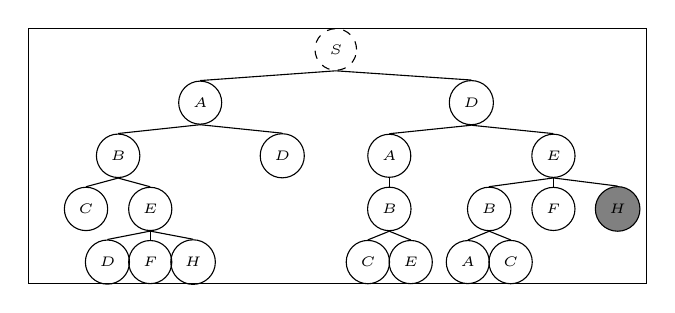
\begin{tikzpicture}[xscale=0.725,yscale=0.9,city/.style={shape=circle,draw=black},cityG/.style={city,very thick},cityM/.style={city,fill=gray}]
\def\dy{-0.75};
\def\dxa{4.75};
\def\dxb{2.875};
\def\dxc{1.125};
\def\dxd{0.75};
\def\dxe{0.75};

\draw (-0.5*\dxa-0.5*\dxb-\dxc-0.45,0.3) rectangle (0.5*\dxa+0.5*\dxb+\dxc+0.5,4*\dy-0.3);

\node[city,dashed] (S) at (0,0) {\tiny $S$};

\node[city] (A) at (-0.5*\dxa,\dy) {\tiny $A$};
\draw (S.south) -- (A.north);
\node[city] (D) at (0.5*\dxa,\dy) {\tiny $D$};
\draw (S.south) -- (D.north);

\node[city] (B) at (-0.5*\dxa-0.5*\dxb,2*\dy) {\tiny $B$};
\draw (A.south) -- (B.north);
\node[city] (D2) at (-0.5*\dxa+0.5*\dxb,2*\dy) {\tiny $D$};
\draw (A.south) -- (D2.north);
\node[city] (A2) at (0.5*\dxa-0.5*\dxb,2*\dy) {\tiny $A$};
\draw (D.south) -- (A2.north);
\node[city] (E) at (0.5*\dxa+0.5*\dxb,2*\dy) {\tiny $E$};
\draw (D.south) -- (E.north);

\node[city] (C) at (-0.5*\dxa-0.5*\dxb-0.5*\dxc,3*\dy) {\tiny $C$};
\draw (B.south) -- (C.north);
\node[city] (E2) at (-0.5*\dxa-0.5*\dxb+0.5*\dxc,3*\dy) {\tiny $E$};
\draw (B.south) -- (E2.north);
\node[city] (B2) at (0.5*\dxa-0.5*\dxb,3*\dy) {\tiny $B$};
\draw (A2.south) -- (B2.north);
\node[city] (B3) at (0.5*\dxa+0.5*\dxb-\dxc,3*\dy) {\tiny $B$};
\draw (E.south) -- (B3.north);
\node[city] (F) at (0.5*\dxa+0.5*\dxb,3*\dy) {\tiny $F$};
\draw (E.south) -- (F.north);
\node[cityM] (H) at (0.5*\dxa+0.5*\dxb+\dxc,3*\dy) {\tiny $H$};
\draw (E.south) -- (H.north);

\node[city] (D3) at (-0.5*\dxa-0.5*\dxb+0.5*\dxc-\dxd,4*\dy) {\tiny $D$};
\draw (E2.south) -- (D3.north);
\node[city] (F2) at (-0.5*\dxa-0.5*\dxb+0.5*\dxc,4*\dy) {\tiny $F$};
\draw (E2.south) -- (F2.north);
\node[city] (H2) at (-0.5*\dxa-0.5*\dxb+0.5*\dxc+\dxd,4*\dy) {\tiny $H$};
\draw (E2.south) -- (H2.north);
\node[city] (C2) at (0.5*\dxa-0.5*\dxb-0.5*\dxd,4*\dy) {\tiny $C$};
\draw (B2.south) -- (C2.north);
\node[city] (E4) at (0.5*\dxa-0.5*\dxb+0.5*\dxd,4*\dy) {\tiny $E$};
\draw (B2.south) -- (E4.north);
\node[city] (A3) at (0.5*\dxa+0.5*\dxb-\dxc-0.5*\dxd,4*\dy) {\tiny $A$};
\draw (B3.south) -- (A3.north);
\node[city] (C3) at (0.5*\dxa+0.5*\dxb-\dxc+0.5*\dxd,4*\dy) {\tiny $C$};
\draw (B3.south) -- (C3.north);
\end{tikzpicture}}
\subfigure{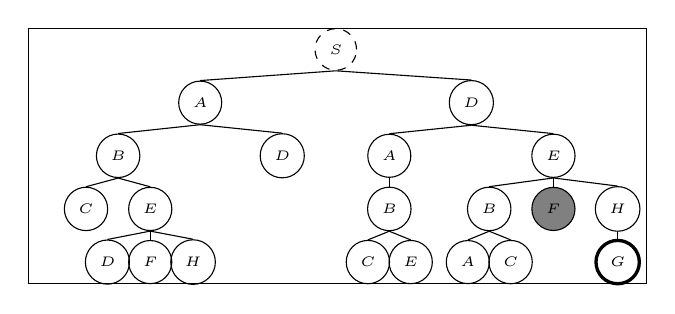
\begin{tikzpicture}[xscale=0.725,yscale=0.9,city/.style={shape=circle,draw=black},cityG/.style={city,very thick},cityM/.style={city,fill=gray}]
\def\dy{-0.75};
\def\dxa{4.75};
\def\dxb{2.875};
\def\dxc{1.125};
\def\dxd{0.75};
\def\dxe{0.75};

\draw (-0.5*\dxa-0.5*\dxb-\dxc-0.45,0.3) rectangle (0.5*\dxa+0.5*\dxb+\dxc+0.5,4*\dy-0.3);

\node[city,dashed] (S) at (0,0) {\tiny $S$};

\node[city] (A) at (-0.5*\dxa,\dy) {\tiny $A$};
\draw (S.south) -- (A.north);
\node[city] (D) at (0.5*\dxa,\dy) {\tiny $D$};
\draw (S.south) -- (D.north);

\node[city] (B) at (-0.5*\dxa-0.5*\dxb,2*\dy) {\tiny $B$};
\draw (A.south) -- (B.north);
\node[city] (D2) at (-0.5*\dxa+0.5*\dxb,2*\dy) {\tiny $D$};
\draw (A.south) -- (D2.north);
\node[city] (A2) at (0.5*\dxa-0.5*\dxb,2*\dy) {\tiny $A$};
\draw (D.south) -- (A2.north);
\node[city] (E) at (0.5*\dxa+0.5*\dxb,2*\dy) {\tiny $E$};
\draw (D.south) -- (E.north);

\node[city] (C) at (-0.5*\dxa-0.5*\dxb-0.5*\dxc,3*\dy) {\tiny $C$};
\draw (B.south) -- (C.north);
\node[city] (E2) at (-0.5*\dxa-0.5*\dxb+0.5*\dxc,3*\dy) {\tiny $E$};
\draw (B.south) -- (E2.north);
\node[city] (B2) at (0.5*\dxa-0.5*\dxb,3*\dy) {\tiny $B$};
\draw (A2.south) -- (B2.north);
\node[city] (B3) at (0.5*\dxa+0.5*\dxb-\dxc,3*\dy) {\tiny $B$};
\draw (E.south) -- (B3.north);
\node[cityM] (F) at (0.5*\dxa+0.5*\dxb,3*\dy) {\tiny $F$};
\draw (E.south) -- (F.north);
\node[city] (H) at (0.5*\dxa+0.5*\dxb+\dxc,3*\dy) {\tiny $H$};
\draw (E.south) -- (H.north);

\node[city] (D3) at (-0.5*\dxa-0.5*\dxb+0.5*\dxc-\dxd,4*\dy) {\tiny $D$};
\draw (E2.south) -- (D3.north);
\node[city] (F2) at (-0.5*\dxa-0.5*\dxb+0.5*\dxc,4*\dy) {\tiny $F$};
\draw (E2.south) -- (F2.north);
\node[city] (H2) at (-0.5*\dxa-0.5*\dxb+0.5*\dxc+\dxd,4*\dy) {\tiny $H$};
\draw (E2.south) -- (H2.north);
\node[city] (C2) at (0.5*\dxa-0.5*\dxb-0.5*\dxd,4*\dy) {\tiny $C$};
\draw (B2.south) -- (C2.north);
\node[city] (E4) at (0.5*\dxa-0.5*\dxb+0.5*\dxd,4*\dy) {\tiny $E$};
\draw (B2.south) -- (E4.north);
\node[city] (A3) at (0.5*\dxa+0.5*\dxb-\dxc-0.5*\dxd,4*\dy) {\tiny $A$};
\draw (B3.south) -- (A3.north);
\node[city] (C3) at (0.5*\dxa+0.5*\dxb-\dxc+0.5*\dxd,4*\dy) {\tiny $C$};
\draw (B3.south) -- (C3.north);
\node[cityG] (G2) at (0.5*\dxa+0.5*\dxb+\dxc,4*\dy) {\tiny $G$};
\draw (H.south) -- (G2.north);
\end{tikzpicture}}
\caption{Een mogelijk scenario van Non-Deterministic Search toegepast op het wegenplan}
\label{fig:nonDeterministicCity}
\end{figure}

\subsection{Heuristic Search Methods}
\begin{figure}[H]
\centering
\subfigure{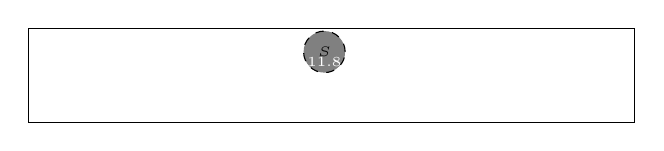
\begin{tikzpicture}[xscale=0.725,yscale=.8,city/.style={shape=circle,draw=black},heurh/.style={yshift=4,gray},heurhM/.style={heurh,white},cityG/.style={city,very thick},cityM/.style={city,fill=gray}]
\def\dy{-0.75};
\def\dxa{4.75};
\def\dxb{2.875};
\def\dxc{1.125};
\def\dxd{0.75};
\def\dxe{0.75};

\draw (-0.5*\dxa-0.5*\dxb-\dxc-0.25,0.375) rectangle (0.5*\dxa+0.5*\dxb+\dxc+0.5,1*\dy-0.375);

\node[cityM,dashed] (S) at (0,0) {\tiny $S$};
\node[heurhM] (Sh) at (S.south) {\tiny 11.8};
\end{tikzpicture}}
\subfigure{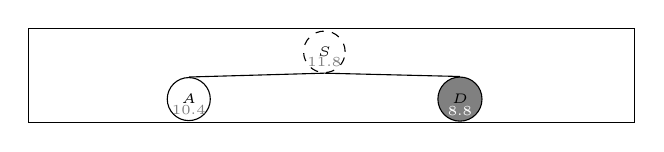
\begin{tikzpicture}[xscale=0.725,yscale=.8,city/.style={shape=circle,draw=black},heurh/.style={yshift=4,gray},heurhM/.style={heurh,white},cityG/.style={city,very thick},cityM/.style={city,fill=gray}]
\def\dy{-0.75};
\def\dxa{4.75};
\def\dxb{2.875};
\def\dxc{1.125};
\def\dxd{0.75};
\def\dxe{0.75};

\draw (-0.5*\dxa-0.5*\dxb-\dxc-0.25,0.375) rectangle (0.5*\dxa+0.5*\dxb+\dxc+0.5,1*\dy-0.375);

\node[city,dashed] (S) at (0,0) {\tiny $S$};
\node[heurh] (Sh) at (S.south) {\tiny 11.8};

\node[city] (A) at (-0.5*\dxa,\dy) {\tiny $A$};
\node[heurh] (Ah) at (A.south) {\tiny 10.4};
\draw (S.south) -- (A.north);
\node[cityM] (D) at (0.5*\dxa,\dy) {\tiny $D$};
\node[heurhM] (Dh) at (D.south) {\tiny 8.8};
\draw (S.south) -- (D.north);
\end{tikzpicture}}
\subfigure{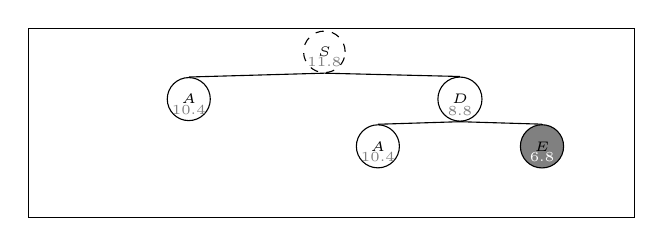
\begin{tikzpicture}[xscale=0.725,yscale=.8,city/.style={shape=circle,draw=black},heurh/.style={yshift=4,gray},heurhM/.style={heurh,white},cityG/.style={city,very thick},cityM/.style={city,fill=gray}]
\def\dy{-0.75};
\def\dxa{4.75};
\def\dxb{2.875};
\def\dxc{1.125};
\def\dxd{0.75};
\def\dxe{0.75};

\draw (-0.5*\dxa-0.5*\dxb-\dxc-0.25,0.375) rectangle (0.5*\dxa+0.5*\dxb+\dxc+0.5,3*\dy-0.375);

\node[city,dashed] (S) at (0,0) {\tiny $S$};
\node[heurh] (Sh) at (S.south) {\tiny 11.8};

\node[city] (A) at (-0.5*\dxa,\dy) {\tiny $A$};
\node[heurh] (Ah) at (A.south) {\tiny 10.4};
\draw (S.south) -- (A.north);
\node[city] (D) at (0.5*\dxa,\dy) {\tiny $D$};
\node[heurh] (Dh) at (D.south) {\tiny 8.8};
\draw (S.south) -- (D.north);

\node[city] (A2) at (0.5*\dxa-0.5*\dxb,2*\dy) {\tiny $A$};
\node[heurh] (A2h) at (A2.south) {\tiny 10.4};
\draw (D.south) -- (A2.north);
\node[cityM] (E) at (0.5*\dxa+0.5*\dxb,2*\dy) {\tiny $E$};
\node[heurhM] (Eh) at (E.south) {\tiny 6.8};
\draw (D.south) -- (E.north);
\end{tikzpicture}}
\subfigure{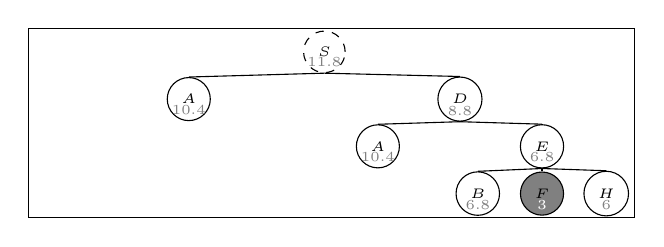
\begin{tikzpicture}[xscale=0.725,yscale=.8,city/.style={shape=circle,draw=black},heurh/.style={yshift=4,gray},heurhM/.style={heurh,white},cityG/.style={city,very thick},cityM/.style={city,fill=gray}]
\def\dy{-0.75};
\def\dxa{4.75};
\def\dxb{2.875};
\def\dxc{1.125};
\def\dxd{0.75};
\def\dxe{0.75};

\draw (-0.5*\dxa-0.5*\dxb-\dxc-0.25,0.375) rectangle (0.5*\dxa+0.5*\dxb+\dxc+0.5,3*\dy-0.375);

\node[city,dashed] (S) at (0,0) {\tiny $S$};
\node[heurh] (Sh) at (S.south) {\tiny 11.8};

\node[city] (A) at (-0.5*\dxa,\dy) {\tiny $A$};
\node[heurh] (Ah) at (A.south) {\tiny 10.4};
\draw (S.south) -- (A.north);
\node[city] (D) at (0.5*\dxa,\dy) {\tiny $D$};
\node[heurh] (Dh) at (D.south) {\tiny 8.8};
\draw (S.south) -- (D.north);

\node[city] (A2) at (0.5*\dxa-0.5*\dxb,2*\dy) {\tiny $A$};
\node[heurh] (A2h) at (A2.south) {\tiny 10.4};
\draw (D.south) -- (A2.north);
\node[city] (E) at (0.5*\dxa+0.5*\dxb,2*\dy) {\tiny $E$};
\node[heurh] (Eh) at (E.south) {\tiny 6.8};
\draw (D.south) -- (E.north);

\node[city] (B3) at (0.5*\dxa+0.5*\dxb-\dxc,3*\dy) {\tiny $B$};
\node[heurh] (B3h) at (B3.south) {\tiny 6.8};
\draw (E.south) -- (B3.north);
\node[cityM] (F) at (0.5*\dxa+0.5*\dxb,3*\dy) {\tiny $F$};
\node[heurhM] (Fh) at (F.south) {\tiny 3};
\draw (E.south) -- (F.north);
\node[city] (H) at (0.5*\dxa+0.5*\dxb+\dxc,3*\dy) {\tiny $H$};
\node[heurh] (Hh) at (H.south) {\tiny 6};
\draw (E.south) -- (H.north);
\end{tikzpicture}}
\subfigure{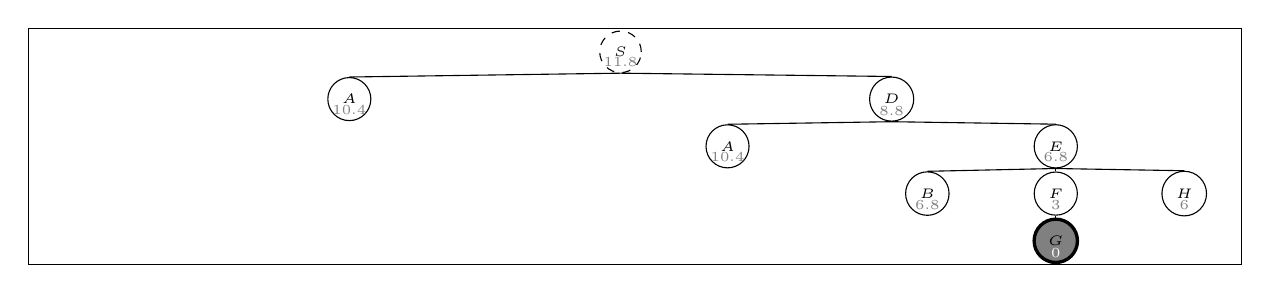
\begin{tikzpicture}[xscale=1.45,yscale=.8,city/.style={shape=circle,draw=black},heurh/.style={yshift=4,gray},heurhM/.style={heurh,white},cityG/.style={city,very thick},cityM/.style={city,fill=gray}]
\def\dy{-0.75};
\def\dxa{4.75};
\def\dxb{2.875};
\def\dxc{1.125};
\def\dxd{0.75};
\def\dxe{0.75};

\draw (-0.5*\dxa-0.5*\dxb-\dxc-0.25,0.375) rectangle (0.5*\dxa+0.5*\dxb+\dxc+0.5,4*\dy-0.375);

\node[city,dashed] (S) at (0,0) {\tiny $S$};
\node[heurh] (Sh) at (S.south) {\tiny 11.8};

\node[city] (A) at (-0.5*\dxa,\dy) {\tiny $A$};
\node[heurh] (Ah) at (A.south) {\tiny 10.4};
\draw (S.south) -- (A.north);
\node[city] (D) at (0.5*\dxa,\dy) {\tiny $D$};
\node[heurh] (Dh) at (D.south) {\tiny 8.8};
\draw (S.south) -- (D.north);

\node[city] (A2) at (0.5*\dxa-0.5*\dxb,2*\dy) {\tiny $A$};
\node[heurh] (A2h) at (A2.south) {\tiny 10.4};
\draw (D.south) -- (A2.north);
\node[city] (E) at (0.5*\dxa+0.5*\dxb,2*\dy) {\tiny $E$};
\node[heurh] (Eh) at (E.south) {\tiny 6.8};
\draw (D.south) -- (E.north);

\node[city] (B3) at (0.5*\dxa+0.5*\dxb-\dxc,3*\dy) {\tiny $B$};
\node[heurh] (B3h) at (B3.south) {\tiny 6.8};
\draw (E.south) -- (B3.north);
\node[city] (F) at (0.5*\dxa+0.5*\dxb,3*\dy) {\tiny $F$};
\node[heurh] (Fh) at (F.south) {\tiny 3};
\draw (E.south) -- (F.north);
\node[city] (H) at (0.5*\dxa+0.5*\dxb+\dxc,3*\dy) {\tiny $H$};
\node[heurh] (Hh) at (H.south) {\tiny 6};
\draw (E.south) -- (H.north);

\node[cityM,cityG] (G) at (0.5*\dxa+0.5*\dxb,4*\dy) {\tiny $G$};
\node[heurhM] (Gh) at (G.south) {\tiny 0};
\draw (F.south) -- (G.north);
\end{tikzpicture}}
\caption{Hill Climbing toegepast op het wegenplan}
\label{fig:hillClimbingCity}
\end{figure}
\begin{figure}[H]
\centering
\subfigure{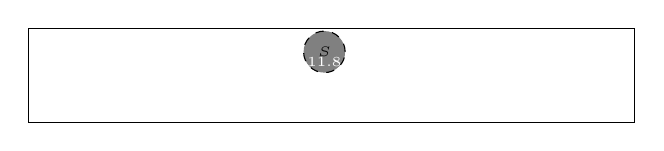
\begin{tikzpicture}[xscale=0.725,yscale=.8,city/.style={shape=circle,draw=black},heurh/.style={yshift=4,gray},heurhM/.style={heurh,white},cityG/.style={city,very thick},cityM/.style={city,fill=gray}]
\def\dy{-0.75};
\def\dxa{4.75};
\def\dxb{2.875};
\def\dxc{1.125};
\def\dxd{0.75};
\def\dxe{0.75};

\draw (-0.5*\dxa-0.5*\dxb-\dxc-0.25,0.375) rectangle (0.5*\dxa+0.5*\dxb+\dxc+0.5,1*\dy-0.375);

\node[cityM,dashed] (S) at (0,0) {\tiny $S$};
\node[heurhM] (Sh) at (S.south) {\tiny 11.8};
\end{tikzpicture}}
\subfigure{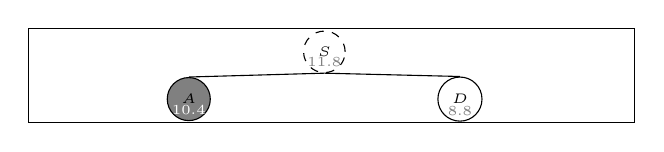
\begin{tikzpicture}[xscale=0.725,yscale=.8,city/.style={shape=circle,draw=black},heurh/.style={yshift=4,gray},heurhM/.style={heurh,white},cityG/.style={city,very thick},cityM/.style={city,fill=gray}]
\def\dy{-0.75};
\def\dxa{4.75};
\def\dxb{2.875};
\def\dxc{1.125};
\def\dxd{0.75};
\def\dxe{0.75};

\draw (-0.5*\dxa-0.5*\dxb-\dxc-0.25,0.375) rectangle (0.5*\dxa+0.5*\dxb+\dxc+0.5,1*\dy-0.375);

\node[city,dashed] (S) at (0,0) {\tiny $S$};
\node[heurh] (Sh) at (S.south) {\tiny 11.8};

\node[cityM] (A) at (-0.5*\dxa,\dy) {\tiny $A$};
\node[heurhM] (Ah) at (A.south) {\tiny 10.4};
\draw (S.south) -- (A.north);
\node[city] (D) at (0.5*\dxa,\dy) {\tiny $D$};
\node[heurh] (Dh) at (D.south) {\tiny 8.8};
\draw (S.south) -- (D.north);
\end{tikzpicture}}
\subfigure{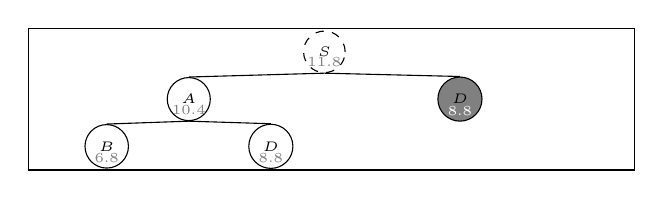
\begin{tikzpicture}[xscale=0.725,yscale=.8,city/.style={shape=circle,draw=black},heurh/.style={yshift=4,gray},heurhM/.style={heurh,white},cityG/.style={city,very thick},cityM/.style={city,fill=gray}]
\def\dy{-0.75};
\def\dxa{4.75};
\def\dxb{2.875};
\def\dxc{1.125};
\def\dxd{0.75};
\def\dxe{0.75};

\draw (-0.5*\dxa-0.5*\dxb-\dxc-0.25,0.375) rectangle (0.5*\dxa+0.5*\dxb+\dxc+0.5,2*\dy-0.375);

\node[city,dashed] (S) at (0,0) {\tiny $S$};
\node[heurh] (Sh) at (S.south) {\tiny 11.8};

\node[city] (A) at (-0.5*\dxa,\dy) {\tiny $A$};
\node[heurh] (Ah) at (A.south) {\tiny 10.4};
\draw (S.south) -- (A.north);
\node[cityM] (D) at (0.5*\dxa,\dy) {\tiny $D$};
\node[heurhM] (Dh) at (D.south) {\tiny 8.8};
\draw (S.south) -- (D.north);

\node[city] (B) at (-0.5*\dxa-0.5*\dxb,2*\dy) {\tiny $B$};
\node[heurh] (Bh) at (B.south) {\tiny 6.8};
\draw (A.south) -- (B.north);
\node[city] (D2) at (-0.5*\dxa+0.5*\dxb,2*\dy) {\tiny $D$};
\node[heurh] (D2h) at (D2.south) {\tiny 8.8};
\draw (A.south) -- (D2.north);
\end{tikzpicture}}
\subfigure{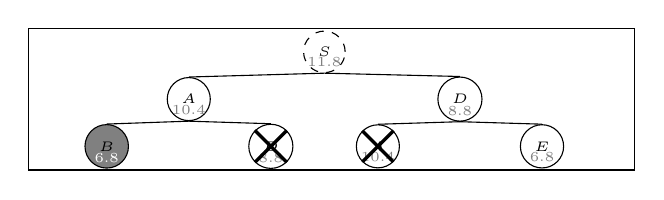
\begin{tikzpicture}[xscale=0.725,yscale=.8,city/.style={shape=circle,draw=black},heurh/.style={yshift=4,gray},heurhM/.style={heurh,white},cityG/.style={city,very thick},cityM/.style={city,fill=gray}]
\def\dy{-0.75};
\def\dxa{4.75};
\def\dxb{2.875};
\def\dxc{1.125};
\def\dxd{0.75};
\def\dxe{0.75};

\draw (-0.5*\dxa-0.5*\dxb-\dxc-0.25,0.375) rectangle (0.5*\dxa+0.5*\dxb+\dxc+0.5,2*\dy-0.375);

\node[city,dashed] (S) at (0,0) {\tiny $S$};
\node[heurh] (Sh) at (S.south) {\tiny 11.8};

\node[city] (A) at (-0.5*\dxa,\dy) {\tiny $A$};
\node[heurh] (Ah) at (A.south) {\tiny 10.4};
\draw (S.south) -- (A.north);
\node[city] (D) at (0.5*\dxa,\dy) {\tiny $D$};
\node[heurh] (Dh) at (D.south) {\tiny 8.8};
\draw (S.south) -- (D.north);

\node[cityM] (B) at (-0.5*\dxa-0.5*\dxb,2*\dy) {\tiny $B$};
\node[heurhM] (Bh) at (B.south) {\tiny 6.8};
\draw (A.south) -- (B.north);
\node[city] (D2) at (-0.5*\dxa+0.5*\dxb,2*\dy) {\tiny $D$};
\node[heurh] (D2h) at (D2.south) {\tiny 8.8};
\draw (A.south) -- (D2.north);
%CROSS D2
\draw[very thick] (D2.north east) -- (D2.south west);
\draw[very thick] (D2.north west) -- (D2.south east);
\node[city] (A2) at (0.5*\dxa-0.5*\dxb,2*\dy) {\tiny $A$};
\node[heurh] (A2h) at (A2.south) {\tiny 10.4};
\draw (D.south) -- (A2.north);
%CROSS A2
\draw[very thick] (A2.north east) -- (A2.south west);
\draw[very thick] (A2.north west) -- (A2.south east);
\node[city] (E) at (0.5*\dxa+0.5*\dxb,2*\dy) {\tiny $E$};
\node[heurh] (Eh) at (E.south) {\tiny 6.8};
\draw (D.south) -- (E.north);
\end{tikzpicture}}
\subfigure{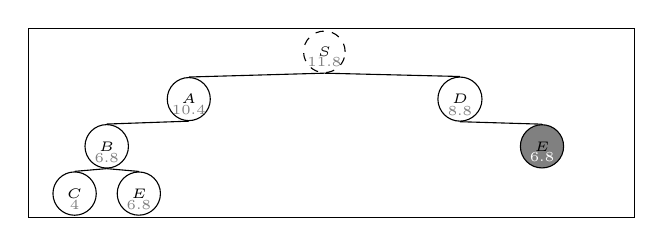
\begin{tikzpicture}[xscale=0.725,yscale=.8,city/.style={shape=circle,draw=black},heurh/.style={yshift=4,gray},heurhM/.style={heurh,white},cityG/.style={city,very thick},cityM/.style={city,fill=gray}]
\def\dy{-0.75};
\def\dxa{4.75};
\def\dxb{2.875};
\def\dxc{1.125};
\def\dxd{0.75};
\def\dxe{0.75};

\draw (-0.5*\dxa-0.5*\dxb-\dxc-0.25,0.375) rectangle (0.5*\dxa+0.5*\dxb+\dxc+0.5,3*\dy-0.375);

\node[city,dashed] (S) at (0,0) {\tiny $S$};
\node[heurh] (Sh) at (S.south) {\tiny 11.8};

\node[city] (A) at (-0.5*\dxa,\dy) {\tiny $A$};
\node[heurh] (Ah) at (A.south) {\tiny 10.4};
\draw (S.south) -- (A.north);
\node[city] (D) at (0.5*\dxa,\dy) {\tiny $D$};
\node[heurh] (Dh) at (D.south) {\tiny 8.8};
\draw (S.south) -- (D.north);

\node[city] (B) at (-0.5*\dxa-0.5*\dxb,2*\dy) {\tiny $B$};
\node[heurh] (Bh) at (B.south) {\tiny 6.8};
\draw (A.south) -- (B.north);
\node[cityM] (E) at (0.5*\dxa+0.5*\dxb,2*\dy) {\tiny $E$};
\node[heurhM] (Eh) at (E.south) {\tiny 6.8};
\draw (D.south) -- (E.north);

\node[city] (C) at (-0.5*\dxa-0.5*\dxb-0.5*\dxc,3*\dy) {\tiny $C$};
\node[heurh] (Ch) at (C.south) {\tiny 4};
\draw (B.south) -- (C.north);
\node[city] (E2) at (-0.5*\dxa-0.5*\dxb+0.5*\dxc,3*\dy) {\tiny $E$};
\node[heurh] (E2h) at (E2.south) {\tiny 6.8};
\draw (B.south) -- (E2.north);
\end{tikzpicture}}
\subfigure{\begin{tikzpicture}[xscale=0.725,yscale=.8,city/.style={shape=circle,draw=black},heurh/.style={yshift=4,gray},heurhM/.style={heurh,white},cityG/.style={city,very thick},cityM/.style={city,fill=gray}]
\def\dy{-0.75};
\def\dxa{4.75};
\def\dxb{2.875};
\def\dxc{1.125};
\def\dxd{0.75};
\def\dxe{0.75};

\draw (-0.5*\dxa-0.5*\dxb-\dxc-0.25,0.375) rectangle (0.5*\dxa+0.5*\dxb+\dxc+0.5,3*\dy-0.375);

\node[city,dashed] (S) at (0,0) {\tiny $S$};
\node[heurh] (Sh) at (S.south) {\tiny 11.8};

\node[city] (A) at (-0.5*\dxa,\dy) {\tiny $A$};
\node[heurh] (Ah) at (A.south) {\tiny 10.4};
\draw (S.south) -- (A.north);
\node[city] (D) at (0.5*\dxa,\dy) {\tiny $D$};
\node[heurh] (Dh) at (D.south) {\tiny 8.8};
\draw (S.south) -- (D.north);

\node[city] (B) at (-0.5*\dxa-0.5*\dxb,2*\dy) {\tiny $B$};
\node[heurh] (Bh) at (B.south) {\tiny 6.8};
\draw (A.south) -- (B.north);
\node[city] (E) at (0.5*\dxa+0.5*\dxb,2*\dy) {\tiny $E$};
\node[heurh] (Eh) at (E.south) {\tiny 6.8};
\draw (D.south) -- (E.north);

\node[cityM] (C) at (-0.5*\dxa-0.5*\dxb-0.5*\dxc,3*\dy) {\tiny $C$};
\node[heurhM] (Ch) at (C.south) {\tiny 4};
\draw (B.south) -- (C.north);
\node[city] (E2) at (-0.5*\dxa-0.5*\dxb+0.5*\dxc,3*\dy) {\tiny $E$};
\node[heurh] (E2h) at (E2.south) {\tiny 6.8};
\draw (B.south) -- (E2.north);
%CROSS E2
\draw[very thick] (E2.north east) -- (E2.south west);
\draw[very thick] (E2.north west) -- (E2.south east);
\node[city] (B3) at (0.5*\dxa+0.5*\dxb-\dxc,3*\dy) {\tiny $B$};
\node[heurh] (B3h) at (B3.south) {\tiny 6.8};
\draw (E.south) -- (B3.north);
%CROSS D2
\draw[very thick] (B3.north east) -- (B3.south west);
\draw[very thick] (B3.north west) -- (B3.south east);
\node[city] (F) at (0.5*\dxa+0.5*\dxb,3*\dy) {\tiny $F$};
\node[heurh] (Fh) at (F.south) {\tiny 3};
\draw (E.south) -- (F.north);
\node[city] (H) at (0.5*\dxa+0.5*\dxb+\dxc,3*\dy) {\tiny $H$};
\node[heurh] (Hh) at (H.south) {\tiny 6};
\draw (E.south) -- (H.north);
%CROSS D2
\draw[very thick] (H.north east) -- (H.south west);
\draw[very thick] (H.north west) -- (H.south east);
\end{tikzpicture}}
\subfigure{\begin{tikzpicture}[xscale=0.725,yscale=.8,city/.style={shape=circle,draw=black},heurh/.style={yshift=4,gray},heurhM/.style={heurh,white},cityG/.style={city,very thick},cityM/.style={city,fill=gray}]
\def\dy{-0.75};
\def\dxa{4.75};
\def\dxb{2.875};
\def\dxc{1.125};
\def\dxd{0.75};
\def\dxe{0.75};

\draw (-0.5*\dxa-0.5*\dxb-\dxc-0.25,0.375) rectangle (0.5*\dxa+0.5*\dxb+\dxc+0.5,4*\dy-0.375);

\node[city,dashed] (S) at (0,0) {\tiny $S$};
\node[heurh] (Sh) at (S.south) {\tiny 11.8};

\node[city] (A) at (-0.5*\dxa,\dy) {\tiny $A$};
\node[heurh] (Ah) at (A.south) {\tiny 10.4};
\draw (S.south) -- (A.north);
\node[city] (D) at (0.5*\dxa,\dy) {\tiny $D$};
\node[heurh] (Dh) at (D.south) {\tiny 8.8};
\draw (S.south) -- (D.north);

\node[city] (B) at (-0.5*\dxa-0.5*\dxb,2*\dy) {\tiny $B$};
\node[heurh] (Bh) at (B.south) {\tiny 6.8};
\draw (A.south) -- (B.north);
\node[city] (E) at (0.5*\dxa+0.5*\dxb,2*\dy) {\tiny $E$};
\node[heurh] (Eh) at (E.south) {\tiny 6.8};
\draw (D.south) -- (E.north);

\node[city] (C) at (-0.5*\dxa-0.5*\dxb-0.5*\dxc,3*\dy) {\tiny $C$};
\node[heurh] (Ch) at (C.south) {\tiny 4};
\draw (B.south) -- (C.north);
\node[cityM] (F) at (0.5*\dxa+0.5*\dxb,3*\dy) {\tiny $F$};
\node[heurhM] (Fh) at (F.south) {\tiny 3};
\draw (E.south) -- (F.north);
\end{tikzpicture}}
\subfigure{\begin{tikzpicture}[xscale=0.725,yscale=.8,city/.style={shape=circle,draw=black},heurh/.style={yshift=4,gray},heurhM/.style={heurh,white},cityG/.style={city,very thick},cityM/.style={city,fill=gray}]
\def\dy{-0.75};
\def\dxa{4.75};
\def\dxb{2.875};
\def\dxc{1.125};
\def\dxd{0.75};
\def\dxe{0.75};

\draw (-0.5*\dxa-0.5*\dxb-\dxc-0.25,0.375) rectangle (0.5*\dxa+0.5*\dxb+\dxc+0.5,4*\dy-0.375);

\node[city,dashed] (S) at (0,0) {\tiny $S$};
\node[heurh] (Sh) at (S.south) {\tiny 11.8};

\node[city] (A) at (-0.5*\dxa,\dy) {\tiny $A$};
\node[heurh] (Ah) at (A.south) {\tiny 10.4};
\draw (S.south) -- (A.north);
\node[city] (D) at (0.5*\dxa,\dy) {\tiny $D$};
\node[heurh] (Dh) at (D.south) {\tiny 8.8};
\draw (S.south) -- (D.north);

\node[city] (B) at (-0.5*\dxa-0.5*\dxb,2*\dy) {\tiny $B$};
\node[heurh] (Bh) at (B.south) {\tiny 6.8};
\draw (A.south) -- (B.north);
\node[city] (E) at (0.5*\dxa+0.5*\dxb,2*\dy) {\tiny $E$};
\node[heurh] (Eh) at (E.south) {\tiny 6.8};
\draw (D.south) -- (E.north);

\node[city] (C) at (-0.5*\dxa-0.5*\dxb-0.5*\dxc,3*\dy) {\tiny $C$};
\node[heurh] (Ch) at (C.south) {\tiny 4};
\draw (B.south) -- (C.north);
\node[city] (F) at (0.5*\dxa+0.5*\dxb,3*\dy) {\tiny $F$};
\node[heurh] (Fh) at (F.south) {\tiny 3};
\draw (E.south) -- (F.north);

\node[cityM,cityG] (G) at (0.5*\dxa+0.5*\dxb,4*\dy) {\tiny $G$};
\node[heurhM] (Gh) at (G.south) {\tiny 0};
\draw (F.south) -- (G.north);
\end{tikzpicture}}
\caption{Beam Search toegepast op het wegenplan (met $w=2$)}
\label{fig:beamSearchCity}
\end{figure}
\begin{figure}[H]
\centering
\subfigure{\begin{tikzpicture}[xscale=0.725,yscale=.8,city/.style={shape=circle,draw=black},heurh/.style={yshift=4,gray},heurhM/.style={heurh,white},cityG/.style={city,very thick},cityM/.style={city,fill=gray}]
\def\dy{-0.75};
\def\dxa{4.75};
\def\dxb{2.875};
\def\dxc{1.125};
\def\dxd{0.75};
\def\dxe{0.75};

\draw (-0.5*\dxa-0.5*\dxb-\dxc-0.25,0.375) rectangle (0.5*\dxa+0.5*\dxb+\dxc+0.5,1*\dy-0.375);

\node[cityM,dashed] (S) at (0,0) {\tiny $S$};
\node[heurhM] (Sh) at (S.south) {\tiny 11.8};
\end{tikzpicture}}
\subfigure{\begin{tikzpicture}[xscale=0.725,yscale=.8,city/.style={shape=circle,draw=black},heurh/.style={yshift=4,gray},heurhM/.style={heurh,white},cityG/.style={city,very thick},cityM/.style={city,fill=gray}]
\def\dy{-0.75};
\def\dxa{4.75};
\def\dxb{2.875};
\def\dxc{1.125};
\def\dxd{0.75};
\def\dxe{0.75};

\draw (-0.5*\dxa-0.5*\dxb-\dxc-0.25,0.375) rectangle (0.5*\dxa+0.5*\dxb+\dxc+0.5,1*\dy-0.375);

\node[city,dashed] (S) at (0,0) {\tiny $S$};
\node[heurh] (Sh) at (S.south) {\tiny 11.8};

\node[city] (A) at (-0.5*\dxa,\dy) {\tiny $A$};
\node[heurh] (Ah) at (A.south) {\tiny 10.4};
\draw (S.south) -- (A.north);
%CROSS A
\draw[very thick] (A.north east) -- (A.south west);
\draw[very thick] (A.north west) -- (A.south east);
\node[cityM] (D) at (0.5*\dxa,\dy) {\tiny $D$};
\node[heurhM] (Dh) at (D.south) {\tiny 8.8};
\draw (S.south) -- (D.north);
\end{tikzpicture}}
\subfigure{\begin{tikzpicture}[xscale=0.725,yscale=.8,city/.style={shape=circle,draw=black},heurh/.style={yshift=4,gray},heurhM/.style={heurh,white},cityG/.style={city,very thick},cityM/.style={city,fill=gray}]
\def\dy{-0.75};
\def\dxa{4.75};
\def\dxb{2.875};
\def\dxc{1.125};
\def\dxd{0.75};
\def\dxe{0.75};

\draw (-0.5*\dxa-0.5*\dxb-\dxc-0.25,0.375) rectangle (0.5*\dxa+0.5*\dxb+\dxc+0.5,3*\dy-0.375);

\node[city,dashed] (S) at (0,0) {\tiny $S$};
\node[heurh] (Sh) at (S.south) {\tiny 11.8};

\node[city] (D) at (0.5*\dxa,\dy) {\tiny $D$};
\node[heurh] (Dh) at (D.south) {\tiny 8.8};
\draw (S.south) -- (D.north);

\node[city] (A2) at (0.5*\dxa-0.5*\dxb,2*\dy) {\tiny $A$};
\node[heurh] (A2h) at (A2.south) {\tiny 10.4};
\draw (D.south) -- (A2.north);
%CROSS A2
\draw[very thick] (A2.north east) -- (A2.south west);
\draw[very thick] (A2.north west) -- (A2.south east);
\node[cityM] (E) at (0.5*\dxa+0.5*\dxb,2*\dy) {\tiny $E$};
\node[heurhM] (Eh) at (E.south) {\tiny 6.8};
\draw (D.south) -- (E.north);
\end{tikzpicture}}
\subfigure{\begin{tikzpicture}[xscale=0.725,yscale=.8,city/.style={shape=circle,draw=black},heurh/.style={yshift=4,gray},heurhM/.style={heurh,white},cityG/.style={city,very thick},cityM/.style={city,fill=gray}]
\def\dy{-0.75};
\def\dxa{4.75};
\def\dxb{2.875};
\def\dxc{1.125};
\def\dxd{0.75};
\def\dxe{0.75};

\draw (-0.5*\dxa-0.5*\dxb-\dxc-0.25,0.375) rectangle (0.5*\dxa+0.5*\dxb+\dxc+0.5,3*\dy-0.375);

\node[city,dashed] (S) at (0,0) {\tiny $S$};
\node[heurh] (Sh) at (S.south) {\tiny 11.8};

\node[city] (D) at (0.5*\dxa,\dy) {\tiny $D$};
\node[heurh] (Dh) at (D.south) {\tiny 8.8};
\draw (S.south) -- (D.north);

\node[city] (E) at (0.5*\dxa+0.5*\dxb,2*\dy) {\tiny $E$};
\node[heurh] (Eh) at (E.south) {\tiny 6.8};
\draw (D.south) -- (E.north);

\node[city] (B3) at (0.5*\dxa+0.5*\dxb-\dxc,3*\dy) {\tiny $B$};
\node[heurh] (B3h) at (B3.south) {\tiny 6.8};
\draw (E.south) -- (B3.north);
%CROSS B3
\draw[very thick] (B3.north east) -- (B3.south west);
\draw[very thick] (B3.north west) -- (B3.south east);
\node[cityM] (F) at (0.5*\dxa+0.5*\dxb,3*\dy) {\tiny $F$};
\node[heurhM] (Fh) at (F.south) {\tiny 3};
\draw (E.south) -- (F.north);
\node[city] (H) at (0.5*\dxa+0.5*\dxb+\dxc,3*\dy) {\tiny $H$};
\node[heurh] (Hh) at (H.south) {\tiny 6};
\draw (E.south) -- (H.north);
%CROSS H
\draw[very thick] (H.north east) -- (H.south west);
\draw[very thick] (H.north west) -- (H.south east);
\end{tikzpicture}}
\subfigure{\begin{tikzpicture}[xscale=1.45,yscale=.8,city/.style={shape=circle,draw=black},heurh/.style={yshift=4,gray},heurhM/.style={heurh,white},cityG/.style={city,very thick},cityM/.style={city,fill=gray}]
\def\dy{-0.75};
\def\dxa{4.75};
\def\dxb{2.875};
\def\dxc{1.125};
\def\dxd{0.75};
\def\dxe{0.75};

\draw (-0.5*\dxa-0.5*\dxb-\dxc-0.25,0.375) rectangle (0.5*\dxa+0.5*\dxb+\dxc+0.5,4*\dy-0.375);

\node[city,dashed] (S) at (0,0) {\tiny $S$};
\node[heurh] (Sh) at (S.south) {\tiny 11.8};

\node[city] (D) at (0.5*\dxa,\dy) {\tiny $D$};
\node[heurh] (Dh) at (D.south) {\tiny 8.8};
\draw (S.south) -- (D.north);

\node[city] (E) at (0.5*\dxa+0.5*\dxb,2*\dy) {\tiny $E$};
\node[heurh] (Eh) at (E.south) {\tiny 6.8};
\draw (D.south) -- (E.north);

\node[city] (F) at (0.5*\dxa+0.5*\dxb,3*\dy) {\tiny $F$};
\node[heurh] (Fh) at (F.south) {\tiny 3};
\draw (E.south) -- (F.north);

\node[cityM,cityG] (G) at (0.5*\dxa+0.5*\dxb,4*\dy) {\tiny $G$};
\node[heurhM] (Gh) at (G.south) {\tiny 0};
\draw (F.south) -- (G.north);
\end{tikzpicture}}
\caption{Hill Climbing 2 toegepast op het wegenplan}
\label{fig:hillClimbing2City}
\end{figure}
\subsection{Optimal Search Methods}
\begin{figure}[H]
\subfigure{\begin{tikzpicture}[xscale=0.725,yscale=0.9,city/.style={shape=circle,draw=black},costc/.style={yshift=-3},heurh/.style={anchor=north east,gray},cityG/.style={city,very thick},cityM/.style={city,fill=gray}]
\def\dy{-0.75};
\def\dxa{4.75};
\def\dxb{2.875};
\def\dxc{1.125};
\def\dxd{0.75};
\def\dxe{0.75};

\draw (-0.5*\dxa-0.5*\dxb-\dxc-0.45,0.3) rectangle (0.5*\dxa+0.5*\dxb+\dxc+0.5,1*\dy-0.3);

\node[cityM,dashed] (S) at (0,0) {\tiny $S$};
\node[costc] (Sc) at (S.north) {\tiny 0};

\end{tikzpicture}}
\subfigure{\begin{tikzpicture}[xscale=0.725,yscale=0.9,city/.style={shape=circle,draw=black},costc/.style={yshift=-3},heurh/.style={anchor=north east,gray},cityG/.style={city,very thick},cityM/.style={city,fill=gray}]
\def\dy{-0.75};
\def\dxa{4.75};
\def\dxb{2.875};
\def\dxc{1.125};
\def\dxd{0.75};
\def\dxe{0.75};

\draw (-0.5*\dxa-0.5*\dxb-\dxc-0.45,0.3) rectangle (0.5*\dxa+0.5*\dxb+\dxc+0.5,1*\dy-0.3);

\node[city,dashed] (S) at (0,0) {\tiny $S$};
\node[costc] (Sc) at (S.north) {\tiny 0};

\node[cityM] (A) at (-0.5*\dxa,\dy) {\tiny $A$};
\node[costc] (Ac) at (A.north) {\tiny 3};
\draw (S.south) -- (A.north);
\node[city] (D) at (0.5*\dxa,\dy) {\tiny $D$};
\node[costc] (Dc) at (D.north) {\tiny 4};
\draw (S.south) -- (D.north);

\end{tikzpicture}}
\subfigure{\begin{tikzpicture}[xscale=0.725,yscale=0.9,city/.style={shape=circle,draw=black},costc/.style={yshift=-3},heurh/.style={anchor=north east,gray},cityG/.style={city,very thick},cityM/.style={city,fill=gray}]
\def\dy{-0.75};
\def\dxa{4.75};
\def\dxb{2.875};
\def\dxc{1.125};
\def\dxd{0.75};
\def\dxe{0.75};

\draw (-0.5*\dxa-0.5*\dxb-\dxc-0.45,0.3) rectangle (0.5*\dxa+0.5*\dxb+\dxc+0.5,2*\dy-0.3);

\node[city,dashed] (S) at (0,0) {\tiny $S$};
\node[costc] (Sc) at (S.north) {\tiny 0};

\node[city] (A) at (-0.5*\dxa,\dy) {\tiny $A$};
\node[costc] (Ac) at (A.north) {\tiny 3};
\draw (S.south) -- (A.north);
\node[cityM] (D) at (0.5*\dxa,\dy) {\tiny $D$};
\node[costc] (Dc) at (D.north) {\tiny 4};
\draw (S.south) -- (D.north);

\node[city] (B) at (-0.5*\dxa-0.5*\dxb,2*\dy) {\tiny $B$};
\node[costc] (Bc) at (B.north) {\tiny 7};
\draw (A.south) -- (B.north);
\node[city] (D2) at (-0.5*\dxa+0.5*\dxb,2*\dy) {\tiny $D$};
\node[costc] (D2c) at (D2.north) {\tiny 8};
\draw (A.south) -- (D2.north);
\end{tikzpicture}}
\subfigure{\begin{tikzpicture}[xscale=0.725,yscale=0.9,city/.style={shape=circle,draw=black},costc/.style={yshift=-3},heurh/.style={anchor=north east,gray},cityG/.style={city,very thick},cityM/.style={city,fill=gray}]
\def\dy{-0.75};
\def\dxa{4.75};
\def\dxb{2.875};
\def\dxc{1.125};
\def\dxd{0.75};
\def\dxe{0.75};

\draw (-0.5*\dxa-0.5*\dxb-\dxc-0.45,0.3) rectangle (0.5*\dxa+0.5*\dxb+\dxc+0.5,2*\dy-0.3);

\node[city,dashed] (S) at (0,0) {\tiny $S$};
\node[costc] (Sc) at (S.north) {\tiny 0};

\node[city] (A) at (-0.5*\dxa,\dy) {\tiny $A$};
\node[costc] (Ac) at (A.north) {\tiny 3};
\draw (S.south) -- (A.north);
\node[city] (D) at (0.5*\dxa,\dy) {\tiny $D$};
\node[costc] (Dc) at (D.north) {\tiny 4};
\draw (S.south) -- (D.north);

\node[city] (B) at (-0.5*\dxa-0.5*\dxb,2*\dy) {\tiny $B$};
\node[costc] (Bc) at (B.north) {\tiny 7};
\draw (A.south) -- (B.north);
\node[city] (D2) at (-0.5*\dxa+0.5*\dxb,2*\dy) {\tiny $D$};
\node[costc] (D2c) at (D2.north) {\tiny 8};
\draw (A.south) -- (D2.north);
\node[city] (A2) at (0.5*\dxa-0.5*\dxb,2*\dy) {\tiny $A$};
\node[costc] (A2c) at (A2.north) {\tiny 9};
\draw (D.south) -- (A2.north);
\node[cityM] (E) at (0.5*\dxa+0.5*\dxb,2*\dy) {\tiny $E$};
\node[costc] (Ec) at (E.north) {\tiny 6};
\draw (D.south) -- (E.north);
\end{tikzpicture}}
\subfigure{\begin{tikzpicture}[xscale=0.725,yscale=0.9,city/.style={shape=circle,draw=black},costc/.style={yshift=-3},heurh/.style={anchor=north east,gray},cityG/.style={city,very thick},cityM/.style={city,fill=gray}]
\def\dy{-0.75};
\def\dxa{4.75};
\def\dxb{2.875};
\def\dxc{1.125};
\def\dxd{0.75};
\def\dxe{0.75};

\draw (-0.5*\dxa-0.5*\dxb-\dxc-0.45,0.3) rectangle (0.5*\dxa+0.5*\dxb+\dxc+0.5,3*\dy-0.3);

\node[city,dashed] (S) at (0,0) {\tiny $S$};
\node[costc] (Sc) at (S.north) {\tiny 0};

\node[city] (A) at (-0.5*\dxa,\dy) {\tiny $A$};
\node[costc] (Ac) at (A.north) {\tiny 3};
\draw (S.south) -- (A.north);
\node[city] (D) at (0.5*\dxa,\dy) {\tiny $D$};
\node[costc] (Dc) at (D.north) {\tiny 4};
\draw (S.south) -- (D.north);

\node[cityM] (B) at (-0.5*\dxa-0.5*\dxb,2*\dy) {\tiny $B$};
\node[costc] (Bc) at (B.north) {\tiny 7};
\draw (A.south) -- (B.north);
\node[city] (D2) at (-0.5*\dxa+0.5*\dxb,2*\dy) {\tiny $D$};
\node[costc] (D2c) at (D2.north) {\tiny 8};
\draw (A.south) -- (D2.north);
\node[city] (A2) at (0.5*\dxa-0.5*\dxb,2*\dy) {\tiny $A$};
\node[costc] (A2c) at (A2.north) {\tiny 9};
\draw (D.south) -- (A2.north);
\node[city] (E) at (0.5*\dxa+0.5*\dxb,2*\dy) {\tiny $E$};
\node[costc] (Ec) at (E.north) {\tiny 6};
\draw (D.south) -- (E.north);

\node[city] (B3) at (0.5*\dxa+0.5*\dxb-\dxc,3*\dy) {\tiny $B$};
\node[costc] (B3c) at (B3.north) {\tiny 11};
\draw (E.south) -- (B3.north);
\node[city] (F) at (0.5*\dxa+0.5*\dxb,3*\dy) {\tiny $F$};
\node[costc] (Fc) at (F.north) {\tiny 10};
\draw (E.south) -- (F.north);
\node[city] (H) at (0.5*\dxa+0.5*\dxb+\dxc,3*\dy) {\tiny $H$};
\node[costc] (Hc) at (H.north) {\tiny 9};
\draw (E.south) -- (H.north);
\end{tikzpicture}}
\subfigure{\begin{tikzpicture}[xscale=0.725,yscale=0.9,city/.style={shape=circle,draw=black},costc/.style={yshift=-3},heurh/.style={anchor=north east,gray},cityG/.style={city,very thick},cityM/.style={city,fill=gray}]
\def\dy{-0.75};
\def\dxa{4.75};
\def\dxb{2.875};
\def\dxc{1.125};
\def\dxd{0.75};
\def\dxe{0.75};

\draw (-0.5*\dxa-0.5*\dxb-\dxc-0.45,0.3) rectangle (0.5*\dxa+0.5*\dxb+\dxc+0.5,3*\dy-0.3);

\node[city,dashed] (S) at (0,0) {\tiny $S$};
\node[costc] (Sc) at (S.north) {\tiny 0};

\node[city] (A) at (-0.5*\dxa,\dy) {\tiny $A$};
\node[costc] (Ac) at (A.north) {\tiny 3};
\draw (S.south) -- (A.north);
\node[city] (D) at (0.5*\dxa,\dy) {\tiny $D$};
\node[costc] (Dc) at (D.north) {\tiny 4};
\draw (S.south) -- (D.north);

\node[city] (B) at (-0.5*\dxa-0.5*\dxb,2*\dy) {\tiny $B$};
\node[costc] (Bc) at (B.north) {\tiny 7};
\draw (A.south) -- (B.north);
\node[cityM] (D2) at (-0.5*\dxa+0.5*\dxb,2*\dy) {\tiny $D$};
\node[costc] (D2c) at (D2.north) {\tiny 8};
\draw (A.south) -- (D2.north);
\node[city] (A2) at (0.5*\dxa-0.5*\dxb,2*\dy) {\tiny $A$};
\node[costc] (A2c) at (A2.north) {\tiny 9};
\draw (D.south) -- (A2.north);
\node[city] (E) at (0.5*\dxa+0.5*\dxb,2*\dy) {\tiny $E$};
\node[costc] (Ec) at (E.north) {\tiny 6};
\draw (D.south) -- (E.north);

\node[city] (C) at (-0.5*\dxa-0.5*\dxb-0.5*\dxc,3*\dy) {\tiny $C$};
\node[costc] (Cc) at (C.north) {\tiny 11};
\draw (B.south) -- (C.north);
\node[city] (E2) at (-0.5*\dxa-0.5*\dxb+0.5*\dxc,3*\dy) {\tiny $E$};
\node[costc] (E2c) at (E2.north) {\tiny 12};
\draw (B.south) -- (E2.north);
\node[city] (B3) at (0.5*\dxa+0.5*\dxb-\dxc,3*\dy) {\tiny $B$};
\node[costc] (B3c) at (B3.north) {\tiny 11};
\draw (E.south) -- (B3.north);
\node[city] (F) at (0.5*\dxa+0.5*\dxb,3*\dy) {\tiny $F$};
\node[costc] (Fc) at (F.north) {\tiny 10};
\draw (E.south) -- (F.north);
\node[city] (H) at (0.5*\dxa+0.5*\dxb+\dxc,3*\dy) {\tiny $H$};
\node[costc] (Hc) at (H.north) {\tiny 9};
\draw (E.south) -- (H.north);
\end{tikzpicture}}
\subfigure{\begin{tikzpicture}[xscale=0.725,yscale=0.9,city/.style={shape=circle,draw=black},costc/.style={yshift=-3},heurh/.style={anchor=north east,gray},cityG/.style={city,very thick},cityM/.style={city,fill=gray}]
\def\dy{-0.75};
\def\dxa{4.75};
\def\dxb{2.875};
\def\dxc{1.125};
\def\dxd{0.75};
\def\dxe{0.75};

\draw (-0.5*\dxa-0.5*\dxb-\dxc-0.45,0.3) rectangle (0.5*\dxa+0.5*\dxb+\dxc+0.5,3*\dy-0.3);

\node[city,dashed] (S) at (0,0) {\tiny $S$};
\node[costc] (Sc) at (S.north) {\tiny 0};

\node[city] (A) at (-0.5*\dxa,\dy) {\tiny $A$};
\node[costc] (Ac) at (A.north) {\tiny 3};
\draw (S.south) -- (A.north);
\node[city] (D) at (0.5*\dxa,\dy) {\tiny $D$};
\node[costc] (Dc) at (D.north) {\tiny 4};
\draw (S.south) -- (D.north);

\node[city] (B) at (-0.5*\dxa-0.5*\dxb,2*\dy) {\tiny $B$};
\node[costc] (Bc) at (B.north) {\tiny 7};
\draw (A.south) -- (B.north);
\node[city] (D2) at (-0.5*\dxa+0.5*\dxb,2*\dy) {\tiny $D$};
\node[costc] (D2c) at (D2.north) {\tiny 8};
\draw (A.south) -- (D2.north);
\node[cityM] (A2) at (0.5*\dxa-0.5*\dxb,2*\dy) {\tiny $A$};
\node[costc] (A2c) at (A2.north) {\tiny 9};
\draw (D.south) -- (A2.north);
\node[city] (E) at (0.5*\dxa+0.5*\dxb,2*\dy) {\tiny $E$};
\node[costc] (Ec) at (E.north) {\tiny 6};
\draw (D.south) -- (E.north);

\node[city] (C) at (-0.5*\dxa-0.5*\dxb-0.5*\dxc,3*\dy) {\tiny $C$};
\node[costc] (Cc) at (C.north) {\tiny 11};
\draw (B.south) -- (C.north);
\node[city] (E2) at (-0.5*\dxa-0.5*\dxb+0.5*\dxc,3*\dy) {\tiny $E$};
\node[costc] (E2c) at (E2.north) {\tiny 12};
\draw (B.south) -- (E2.north);
\node[city] (E3) at (-0.5*\dxa+0.5*\dxb,3*\dy) {\tiny $E$};
\node[costc] (E3c) at (E3.north) {\tiny 10};
\draw (D2.south) -- (E3.north);
\node[city] (B3) at (0.5*\dxa+0.5*\dxb-\dxc,3*\dy) {\tiny $B$};
\node[costc] (B3c) at (B3.north) {\tiny 11};
\draw (E.south) -- (B3.north);
\node[city] (F) at (0.5*\dxa+0.5*\dxb,3*\dy) {\tiny $F$};
\node[costc] (Fc) at (F.north) {\tiny 10};
\draw (E.south) -- (F.north);
\node[city] (H) at (0.5*\dxa+0.5*\dxb+\dxc,3*\dy) {\tiny $H$};
\node[costc] (Hc) at (H.north) {\tiny 9};
\draw (E.south) -- (H.north);
\end{tikzpicture}}
\subfigure{\begin{tikzpicture}[xscale=0.725,yscale=0.9,city/.style={shape=circle,draw=black},costc/.style={yshift=-3},heurh/.style={anchor=north east,gray},cityG/.style={city,very thick},cityM/.style={city,fill=gray}]
\def\dy{-0.75};
\def\dxa{4.75};
\def\dxb{2.875};
\def\dxc{1.125};
\def\dxd{0.75};
\def\dxe{0.75};

\draw (-0.5*\dxa-0.5*\dxb-\dxc-0.45,0.3) rectangle (0.5*\dxa+0.5*\dxb+\dxc+0.5,3*\dy-0.3);

\node[city,dashed] (S) at (0,0) {\tiny $S$};
\node[costc] (Sc) at (S.north) {\tiny 0};

\node[city] (A) at (-0.5*\dxa,\dy) {\tiny $A$};
\node[costc] (Ac) at (A.north) {\tiny 3};
\draw (S.south) -- (A.north);
\node[city] (D) at (0.5*\dxa,\dy) {\tiny $D$};
\node[costc] (Dc) at (D.north) {\tiny 4};
\draw (S.south) -- (D.north);

\node[city] (B) at (-0.5*\dxa-0.5*\dxb,2*\dy) {\tiny $B$};
\node[costc] (Bc) at (B.north) {\tiny 7};
\draw (A.south) -- (B.north);
\node[city] (D2) at (-0.5*\dxa+0.5*\dxb,2*\dy) {\tiny $D$};
\node[costc] (D2c) at (D2.north) {\tiny 8};
\draw (A.south) -- (D2.north);
\node[city] (A2) at (0.5*\dxa-0.5*\dxb,2*\dy) {\tiny $A$};
\node[costc] (A2c) at (A2.north) {\tiny 9};
\draw (D.south) -- (A2.north);
\node[city] (E) at (0.5*\dxa+0.5*\dxb,2*\dy) {\tiny $E$};
\node[costc] (Ec) at (E.north) {\tiny 6};
\draw (D.south) -- (E.north);

\node[city] (C) at (-0.5*\dxa-0.5*\dxb-0.5*\dxc,3*\dy) {\tiny $C$};
\node[costc] (Cc) at (C.north) {\tiny 11};
\draw (B.south) -- (C.north);
\node[city] (E2) at (-0.5*\dxa-0.5*\dxb+0.5*\dxc,3*\dy) {\tiny $E$};
\node[costc] (E2c) at (E2.north) {\tiny 12};
\draw (B.south) -- (E2.north);
\node[city] (E3) at (-0.5*\dxa+0.5*\dxb,3*\dy) {\tiny $E$};
\node[costc] (E3c) at (E3.north) {\tiny 10};
\draw (D2.south) -- (E3.north);
\node[city] (B2) at (0.5*\dxa-0.5*\dxb,3*\dy) {\tiny $B$};
\node[costc] (B2c) at (B2.north) {\tiny 13};
\draw (A2.south) -- (B2.north);
\node[city] (B3) at (0.5*\dxa+0.5*\dxb-\dxc,3*\dy) {\tiny $B$};
\node[costc] (B3c) at (B3.north) {\tiny 11};
\draw (E.south) -- (B3.north);
\node[city] (F) at (0.5*\dxa+0.5*\dxb,3*\dy) {\tiny $F$};
\node[costc] (Fc) at (F.north) {\tiny 10};
\draw (E.south) -- (F.north);
\node[cityM] (H) at (0.5*\dxa+0.5*\dxb+\dxc,3*\dy) {\tiny $H$};
\node[costc] (Hc) at (H.north) {\tiny 9};
\draw (E.south) -- (H.north);
\end{tikzpicture}}
\centering
\subfigure{\begin{tikzpicture}[xscale=1.45,yscale=0.9,city/.style={shape=circle,draw=black},costc/.style={yshift=-3},heurh/.style={anchor=north east,gray},cityG/.style={city,very thick},cityM/.style={city,fill=gray}]
\def\dy{-0.75};
\def\dxa{4.75};
\def\dxb{2.875};
\def\dxc{1.125};
\def\dxd{0.75};
\def\dxe{0.75};

\draw (-0.5*\dxa-0.5*\dxb-\dxc-0.45,0.3) rectangle (0.5*\dxa+0.5*\dxb+\dxc+0.5,4*\dy-0.3);

\node[city,dashed] (S) at (0,0) {\tiny $S$};
\node[costc] (Sc) at (S.north) {\tiny 0};

\node[city] (A) at (-0.5*\dxa,\dy) {\tiny $A$};
\node[costc] (Ac) at (A.north) {\tiny 3};
\draw (S.south) -- (A.north);
\node[city] (D) at (0.5*\dxa,\dy) {\tiny $D$};
\node[costc] (Dc) at (D.north) {\tiny 4};
\draw (S.south) -- (D.north);

\node[city] (B) at (-0.5*\dxa-0.5*\dxb,2*\dy) {\tiny $B$};
\node[costc] (Bc) at (B.north) {\tiny 7};
\draw (A.south) -- (B.north);
\node[city] (D2) at (-0.5*\dxa+0.5*\dxb,2*\dy) {\tiny $D$};
\node[costc] (D2c) at (D2.north) {\tiny 8};
\draw (A.south) -- (D2.north);
\node[city] (A2) at (0.5*\dxa-0.5*\dxb,2*\dy) {\tiny $A$};
\node[costc] (A2c) at (A2.north) {\tiny 9};
\draw (D.south) -- (A2.north);
\node[city] (E) at (0.5*\dxa+0.5*\dxb,2*\dy) {\tiny $E$};
\node[costc] (Ec) at (E.north) {\tiny 6};
\draw (D.south) -- (E.north);

\node[city] (C) at (-0.5*\dxa-0.5*\dxb-0.5*\dxc,3*\dy) {\tiny $C$};
\node[costc] (Cc) at (C.north) {\tiny 11};
\draw (B.south) -- (C.north);
\node[city] (E2) at (-0.5*\dxa-0.5*\dxb+0.5*\dxc,3*\dy) {\tiny $E$};
\node[costc] (E2c) at (E2.north) {\tiny 12};
\draw (B.south) -- (E2.north);
\node[city] (E3) at (-0.5*\dxa+0.5*\dxb,3*\dy) {\tiny $E$};
\node[costc] (E3c) at (E3.north) {\tiny 10};
\draw (D2.south) -- (E3.north);
\node[city] (B2) at (0.5*\dxa-0.5*\dxb,3*\dy) {\tiny $B$};
\node[costc] (B2c) at (B2.north) {\tiny 13};
\draw (A2.south) -- (B2.north);
\node[city] (B3) at (0.5*\dxa+0.5*\dxb-\dxc,3*\dy) {\tiny $B$};
\node[costc] (B3c) at (B3.north) {\tiny 11};
\draw (E.south) -- (B3.north);
\node[cityM] (F) at (0.5*\dxa+0.5*\dxb,3*\dy) {\tiny $F$};
\node[costc] (Fc) at (F.north) {\tiny 10};
\draw (E.south) -- (F.north);
\node[city] (H) at (0.5*\dxa+0.5*\dxb+\dxc,3*\dy) {\tiny $H$};
\node[costc] (Hc) at (H.north) {\tiny 9};
\draw (E.south) -- (H.north);

\node[cityG] (G2) at (0.5*\dxa+0.5*\dxb+\dxc,4*\dy) {\tiny $G$};
\node[costc] (G2c) at (G2.north) {\tiny 15};
\draw (H.south) -- (G2.north);
\end{tikzpicture}}
\caption{Uniform Cost Search toegepast op het wegenplan}
\label{fig:uniformCostCity}
\end{figure}
\begin{figure}[H]
\centering
\subfigure{\begin{tikzpicture}[xscale=0.725,yscale=.8,city/.style={shape=circle,draw=black},costc/.style={yshift=-3},heurh/.style={anchor=north east,gray},cityG/.style={city,very thick},cityM/.style={city,fill=gray}]
\def\dy{-0.75};
\def\dxa{4.75};
\def\dxb{2.875};
\def\dxc{1.125};
\def\dxd{0.75};
\def\dxe{0.75};

\draw (-0.5*\dxa-0.5*\dxb-\dxc-0.45,0.35) rectangle (0.5*\dxa+0.5*\dxb+\dxc+0.5,1*\dy-0.35);

\node[cityM,dashed] (S) at (0,0) {\tiny $S$};
\node[costc] (Sc) at (S.north) {\tiny 0};

\end{tikzpicture}}
\subfigure{\begin{tikzpicture}[xscale=0.725,yscale=.8,city/.style={shape=circle,draw=black},costc/.style={yshift=-3},heurh/.style={anchor=north east,gray},cityG/.style={city,very thick},cityM/.style={city,fill=gray}]
\def\dy{-0.75};
\def\dxa{4.75};
\def\dxb{2.875};
\def\dxc{1.125};
\def\dxd{0.75};
\def\dxe{0.75};

\draw (-0.5*\dxa-0.5*\dxb-\dxc-0.45,0.35) rectangle (0.5*\dxa+0.5*\dxb+\dxc+0.5,1*\dy-0.35);

\node[city,dashed] (S) at (0,0) {\tiny $S$};
\node[costc] (Sc) at (S.north) {\tiny 0};

\node[cityM] (A) at (-0.5*\dxa,\dy) {\tiny $A$};
\node[costc] (Ac) at (A.north) {\tiny 3};
\draw (S.south) -- (A.north);
\node[city] (D) at (0.5*\dxa,\dy) {\tiny $D$};
\node[costc] (Dc) at (D.north) {\tiny 4};
\draw (S.south) -- (D.north);

\end{tikzpicture}}
\subfigure{\begin{tikzpicture}[xscale=0.725,yscale=.8,city/.style={shape=circle,draw=black},costc/.style={yshift=-3},heurh/.style={anchor=north east,gray},cityG/.style={city,very thick},cityM/.style={city,fill=gray}]
\def\dy{-0.75};
\def\dxa{4.75};
\def\dxb{2.875};
\def\dxc{1.125};
\def\dxd{0.75};
\def\dxe{0.75};

\draw (-0.5*\dxa-0.5*\dxb-\dxc-0.45,0.35) rectangle (0.5*\dxa+0.5*\dxb+\dxc+0.5,2*\dy-0.35);

\node[city,dashed] (S) at (0,0) {\tiny $S$};
\node[costc] (Sc) at (S.north) {\tiny 0};

\node[city] (A) at (-0.5*\dxa,\dy) {\tiny $A$};
\node[costc] (Ac) at (A.north) {\tiny 3};
\draw (S.south) -- (A.north);
\node[cityM] (D) at (0.5*\dxa,\dy) {\tiny $D$};
\node[costc] (Dc) at (D.north) {\tiny 4};
\draw (S.south) -- (D.north);

\node[city] (B) at (-0.5*\dxa-0.5*\dxb,2*\dy) {\tiny $B$};
\node[costc] (Bc) at (B.north) {\tiny 7};
\draw (A.south) -- (B.north);
\node[city] (D2) at (-0.5*\dxa+0.5*\dxb,2*\dy) {\tiny $D$};
\node[costc] (D2c) at (D2.north) {\tiny 8};
\draw (A.south) -- (D2.north);
\end{tikzpicture}}
\subfigure{\begin{tikzpicture}[xscale=0.725,yscale=.8,city/.style={shape=circle,draw=black},costc/.style={yshift=-3},heurh/.style={anchor=north east,gray},cityG/.style={city,very thick},cityM/.style={city,fill=gray}]
\def\dy{-0.75};
\def\dxa{4.75};
\def\dxb{2.875};
\def\dxc{1.125};
\def\dxd{0.75};
\def\dxe{0.75};

\draw (-0.5*\dxa-0.5*\dxb-\dxc-0.45,0.35) rectangle (0.5*\dxa+0.5*\dxb+\dxc+0.5,2*\dy-0.35);

\node[city,dashed] (S) at (0,0) {\tiny $S$};
\node[costc] (Sc) at (S.north) {\tiny 0};

\node[city] (A) at (-0.5*\dxa,\dy) {\tiny $A$};
\node[costc] (Ac) at (A.north) {\tiny 3};
\draw (S.south) -- (A.north);
\node[city] (D) at (0.5*\dxa,\dy) {\tiny $D$};
\node[costc] (Dc) at (D.north) {\tiny 4};
\draw (S.south) -- (D.north);

\node[city] (B) at (-0.5*\dxa-0.5*\dxb,2*\dy) {\tiny $B$};
\node[costc] (Bc) at (B.north) {\tiny 7};
\draw (A.south) -- (B.north);
\node[city] (D2) at (-0.5*\dxa+0.5*\dxb,2*\dy) {\tiny $D$};
\node[costc] (D2c) at (D2.north) {\tiny 8};
\draw (A.south) -- (D2.north);
\node[city] (A2) at (0.5*\dxa-0.5*\dxb,2*\dy) {\tiny $A$};
\node[costc] (A2c) at (A2.north) {\tiny 9};
\draw (D.south) -- (A2.north);
\node[cityM] (E) at (0.5*\dxa+0.5*\dxb,2*\dy) {\tiny $E$};
\node[costc] (Ec) at (E.north) {\tiny 6};
\draw (D.south) -- (E.north);
\end{tikzpicture}}
\subfigure{\begin{tikzpicture}[xscale=0.725,yscale=.8,city/.style={shape=circle,draw=black},costc/.style={yshift=-3},heurh/.style={anchor=north east,gray},cityG/.style={city,very thick},cityM/.style={city,fill=gray}]
\def\dy{-0.75};
\def\dxa{4.75};
\def\dxb{2.875};
\def\dxc{1.125};
\def\dxd{0.75};
\def\dxe{0.75};

\draw (-0.5*\dxa-0.5*\dxb-\dxc-0.45,0.35) rectangle (0.5*\dxa+0.5*\dxb+\dxc+0.5,3*\dy-0.35);

\node[city,dashed] (S) at (0,0) {\tiny $S$};
\node[costc] (Sc) at (S.north) {\tiny 0};

\node[city] (A) at (-0.5*\dxa,\dy) {\tiny $A$};
\node[costc] (Ac) at (A.north) {\tiny 3};
\draw (S.south) -- (A.north);
\node[city] (D) at (0.5*\dxa,\dy) {\tiny $D$};
\node[costc] (Dc) at (D.north) {\tiny 4};
\draw (S.south) -- (D.north);

\node[cityM] (B) at (-0.5*\dxa-0.5*\dxb,2*\dy) {\tiny $B$};
\node[costc] (Bc) at (B.north) {\tiny 7};
\draw (A.south) -- (B.north);
\node[city] (D2) at (-0.5*\dxa+0.5*\dxb,2*\dy) {\tiny $D$};
\node[costc] (D2c) at (D2.north) {\tiny 8};
\draw (A.south) -- (D2.north);
\node[city] (A2) at (0.5*\dxa-0.5*\dxb,2*\dy) {\tiny $A$};
\node[costc] (A2c) at (A2.north) {\tiny 9};
\draw (D.south) -- (A2.north);
\node[city] (E) at (0.5*\dxa+0.5*\dxb,2*\dy) {\tiny $E$};
\node[costc] (Ec) at (E.north) {\tiny 6};
\draw (D.south) -- (E.north);

\node[city] (B3) at (0.5*\dxa+0.5*\dxb-\dxc,3*\dy) {\tiny $B$};
\node[costc] (B3c) at (B3.north) {\tiny 11};
\draw (E.south) -- (B3.north);
\node[city] (F) at (0.5*\dxa+0.5*\dxb,3*\dy) {\tiny $F$};
\node[costc] (Fc) at (F.north) {\tiny 10};
\draw (E.south) -- (F.north);
\node[city] (H) at (0.5*\dxa+0.5*\dxb+\dxc,3*\dy) {\tiny $H$};
\node[costc] (Hc) at (H.north) {\tiny 9};
\draw (E.south) -- (H.north);
\end{tikzpicture}}
\subfigure{\begin{tikzpicture}[xscale=0.725,yscale=.8,city/.style={shape=circle,draw=black},costc/.style={yshift=-3},heurh/.style={anchor=north east,gray},cityG/.style={city,very thick},cityM/.style={city,fill=gray}]
\def\dy{-0.75};
\def\dxa{4.75};
\def\dxb{2.875};
\def\dxc{1.125};
\def\dxd{0.75};
\def\dxe{0.75};

\draw (-0.5*\dxa-0.5*\dxb-\dxc-0.45,0.35) rectangle (0.5*\dxa+0.5*\dxb+\dxc+0.5,3*\dy-0.35);

\node[city,dashed] (S) at (0,0) {\tiny $S$};
\node[costc] (Sc) at (S.north) {\tiny 0};

\node[city] (A) at (-0.5*\dxa,\dy) {\tiny $A$};
\node[costc] (Ac) at (A.north) {\tiny 3};
\draw (S.south) -- (A.north);
\node[city] (D) at (0.5*\dxa,\dy) {\tiny $D$};
\node[costc] (Dc) at (D.north) {\tiny 4};
\draw (S.south) -- (D.north);

\node[city] (B) at (-0.5*\dxa-0.5*\dxb,2*\dy) {\tiny $B$};
\node[costc] (Bc) at (B.north) {\tiny 7};
\draw (A.south) -- (B.north);
\node[cityM] (D2) at (-0.5*\dxa+0.5*\dxb,2*\dy) {\tiny $D$};
\node[costc] (D2c) at (D2.north) {\tiny 8};
\draw (A.south) -- (D2.north);
\node[city] (A2) at (0.5*\dxa-0.5*\dxb,2*\dy) {\tiny $A$};
\node[costc] (A2c) at (A2.north) {\tiny 9};
\draw (D.south) -- (A2.north);
\node[city] (E) at (0.5*\dxa+0.5*\dxb,2*\dy) {\tiny $E$};
\node[costc] (Ec) at (E.north) {\tiny 6};
\draw (D.south) -- (E.north);

\node[city] (C) at (-0.5*\dxa-0.5*\dxb-0.5*\dxc,3*\dy) {\tiny $C$};
\node[costc] (Cc) at (C.north) {\tiny 11};
\draw (B.south) -- (C.north);
\node[city] (E2) at (-0.5*\dxa-0.5*\dxb+0.5*\dxc,3*\dy) {\tiny $E$};
\node[costc] (E2c) at (E2.north) {\tiny 12};
\draw (B.south) -- (E2.north);
\node[city] (B3) at (0.5*\dxa+0.5*\dxb-\dxc,3*\dy) {\tiny $B$};
\node[costc] (B3c) at (B3.north) {\tiny 11};
\draw (E.south) -- (B3.north);
\node[city] (F) at (0.5*\dxa+0.5*\dxb,3*\dy) {\tiny $F$};
\node[costc] (Fc) at (F.north) {\tiny 10};
\draw (E.south) -- (F.north);
\node[city] (H) at (0.5*\dxa+0.5*\dxb+\dxc,3*\dy) {\tiny $H$};
\node[costc] (Hc) at (H.north) {\tiny 9};
\draw (E.south) -- (H.north);
\end{tikzpicture}}
\subfigure{\begin{tikzpicture}[xscale=0.725,yscale=.8,city/.style={shape=circle,draw=black},costc/.style={yshift=-3},heurh/.style={anchor=north east,gray},cityG/.style={city,very thick},cityM/.style={city,fill=gray}]
\def\dy{-0.75};
\def\dxa{4.75};
\def\dxb{2.875};
\def\dxc{1.125};
\def\dxd{0.75};
\def\dxe{0.75};

\draw (-0.5*\dxa-0.5*\dxb-\dxc-0.45,0.35) rectangle (0.5*\dxa+0.5*\dxb+\dxc+0.5,3*\dy-0.35);

\node[city,dashed] (S) at (0,0) {\tiny $S$};
\node[costc] (Sc) at (S.north) {\tiny 0};

\node[city] (A) at (-0.5*\dxa,\dy) {\tiny $A$};
\node[costc] (Ac) at (A.north) {\tiny 3};
\draw (S.south) -- (A.north);
\node[city] (D) at (0.5*\dxa,\dy) {\tiny $D$};
\node[costc] (Dc) at (D.north) {\tiny 4};
\draw (S.south) -- (D.north);

\node[city] (B) at (-0.5*\dxa-0.5*\dxb,2*\dy) {\tiny $B$};
\node[costc] (Bc) at (B.north) {\tiny 7};
\draw (A.south) -- (B.north);
\node[city] (D2) at (-0.5*\dxa+0.5*\dxb,2*\dy) {\tiny $D$};
\node[costc] (D2c) at (D2.north) {\tiny 8};
\draw (A.south) -- (D2.north);
\node[cityM] (A2) at (0.5*\dxa-0.5*\dxb,2*\dy) {\tiny $A$};
\node[costc] (A2c) at (A2.north) {\tiny 9};
\draw (D.south) -- (A2.north);
\node[city] (E) at (0.5*\dxa+0.5*\dxb,2*\dy) {\tiny $E$};
\node[costc] (Ec) at (E.north) {\tiny 6};
\draw (D.south) -- (E.north);

\node[city] (C) at (-0.5*\dxa-0.5*\dxb-0.5*\dxc,3*\dy) {\tiny $C$};
\node[costc] (Cc) at (C.north) {\tiny 11};
\draw (B.south) -- (C.north);
\node[city] (E2) at (-0.5*\dxa-0.5*\dxb+0.5*\dxc,3*\dy) {\tiny $E$};
\node[costc] (E2c) at (E2.north) {\tiny 12};
\draw (B.south) -- (E2.north);
\node[city] (E3) at (-0.5*\dxa+0.5*\dxb,3*\dy) {\tiny $E$};
\node[costc] (E3c) at (E3.north) {\tiny 10};
\draw (D2.south) -- (E3.north);
\node[city] (B3) at (0.5*\dxa+0.5*\dxb-\dxc,3*\dy) {\tiny $B$};
\node[costc] (B3c) at (B3.north) {\tiny 11};
\draw (E.south) -- (B3.north);
\node[city] (F) at (0.5*\dxa+0.5*\dxb,3*\dy) {\tiny $F$};
\node[costc] (Fc) at (F.north) {\tiny 10};
\draw (E.south) -- (F.north);
\node[city] (H) at (0.5*\dxa+0.5*\dxb+\dxc,3*\dy) {\tiny $H$};
\node[costc] (Hc) at (H.north) {\tiny 9};
\draw (E.south) -- (H.north);
\end{tikzpicture}}
\subfigure{\begin{tikzpicture}[xscale=0.725,yscale=.8,city/.style={shape=circle,draw=black},costc/.style={yshift=-3},heurh/.style={anchor=north east,gray},cityG/.style={city,very thick},cityM/.style={city,fill=gray}]
\def\dy{-0.75};
\def\dxa{4.75};
\def\dxb{2.875};
\def\dxc{1.125};
\def\dxd{0.75};
\def\dxe{0.75};

\draw (-0.5*\dxa-0.5*\dxb-\dxc-0.45,0.35) rectangle (0.5*\dxa+0.5*\dxb+\dxc+0.5,3*\dy-0.35);

\node[city,dashed] (S) at (0,0) {\tiny $S$};
\node[costc] (Sc) at (S.north) {\tiny 0};

\node[city] (A) at (-0.5*\dxa,\dy) {\tiny $A$};
\node[costc] (Ac) at (A.north) {\tiny 3};
\draw (S.south) -- (A.north);
\node[city] (D) at (0.5*\dxa,\dy) {\tiny $D$};
\node[costc] (Dc) at (D.north) {\tiny 4};
\draw (S.south) -- (D.north);

\node[city] (B) at (-0.5*\dxa-0.5*\dxb,2*\dy) {\tiny $B$};
\node[costc] (Bc) at (B.north) {\tiny 7};
\draw (A.south) -- (B.north);
\node[city] (D2) at (-0.5*\dxa+0.5*\dxb,2*\dy) {\tiny $D$};
\node[costc] (D2c) at (D2.north) {\tiny 8};
\draw (A.south) -- (D2.north);
\node[city] (A2) at (0.5*\dxa-0.5*\dxb,2*\dy) {\tiny $A$};
\node[costc] (A2c) at (A2.north) {\tiny 9};
\draw (D.south) -- (A2.north);
\node[city] (E) at (0.5*\dxa+0.5*\dxb,2*\dy) {\tiny $E$};
\node[costc] (Ec) at (E.north) {\tiny 6};
\draw (D.south) -- (E.north);

\node[city] (C) at (-0.5*\dxa-0.5*\dxb-0.5*\dxc,3*\dy) {\tiny $C$};
\node[costc] (Cc) at (C.north) {\tiny 11};
\draw (B.south) -- (C.north);
\node[city] (E2) at (-0.5*\dxa-0.5*\dxb+0.5*\dxc,3*\dy) {\tiny $E$};
\node[costc] (E2c) at (E2.north) {\tiny 12};
\draw (B.south) -- (E2.north);
\node[city] (E3) at (-0.5*\dxa+0.5*\dxb,3*\dy) {\tiny $E$};
\node[costc] (E3c) at (E3.north) {\tiny 10};
\draw (D2.south) -- (E3.north);
\node[city] (B2) at (0.5*\dxa-0.5*\dxb,3*\dy) {\tiny $B$};
\node[costc] (B2c) at (B2.north) {\tiny 13};
\draw (A2.south) -- (B2.north);
\node[city] (B3) at (0.5*\dxa+0.5*\dxb-\dxc,3*\dy) {\tiny $B$};
\node[costc] (B3c) at (B3.north) {\tiny 11};
\draw (E.south) -- (B3.north);
\node[city] (F) at (0.5*\dxa+0.5*\dxb,3*\dy) {\tiny $F$};
\node[costc] (Fc) at (F.north) {\tiny 10};
\draw (E.south) -- (F.north);
\node[cityM] (H) at (0.5*\dxa+0.5*\dxb+\dxc,3*\dy) {\tiny $H$};
\node[costc] (Hc) at (H.north) {\tiny 9};
\draw (E.south) -- (H.north);
\end{tikzpicture}}
\subfigure{\begin{tikzpicture}[xscale=0.725,yscale=.8,city/.style={shape=circle,draw=black},costc/.style={yshift=-3},heurh/.style={anchor=north east,gray},cityG/.style={city,very thick},cityM/.style={city,fill=gray}]
\def\dy{-0.75};
\def\dxa{4.75};
\def\dxb{2.875};
\def\dxc{1.125};
\def\dxd{0.75};
\def\dxe{0.75};

\draw (-0.5*\dxa-0.5*\dxb-\dxc-0.45,0.35) rectangle (0.5*\dxa+0.5*\dxb+\dxc+0.5,4*\dy-0.35);

\node[city,dashed] (S) at (0,0) {\tiny $S$};
\node[costc] (Sc) at (S.north) {\tiny 0};

\node[city] (A) at (-0.5*\dxa,\dy) {\tiny $A$};
\node[costc] (Ac) at (A.north) {\tiny 3};
\draw (S.south) -- (A.north);
\node[city] (D) at (0.5*\dxa,\dy) {\tiny $D$};
\node[costc] (Dc) at (D.north) {\tiny 4};
\draw (S.south) -- (D.north);

\node[city] (B) at (-0.5*\dxa-0.5*\dxb,2*\dy) {\tiny $B$};
\node[costc] (Bc) at (B.north) {\tiny 7};
\draw (A.south) -- (B.north);
\node[city] (D2) at (-0.5*\dxa+0.5*\dxb,2*\dy) {\tiny $D$};
\node[costc] (D2c) at (D2.north) {\tiny 8};
\draw (A.south) -- (D2.north);
\node[city] (A2) at (0.5*\dxa-0.5*\dxb,2*\dy) {\tiny $A$};
\node[costc] (A2c) at (A2.north) {\tiny 9};
\draw (D.south) -- (A2.north);
\node[city] (E) at (0.5*\dxa+0.5*\dxb,2*\dy) {\tiny $E$};
\node[costc] (Ec) at (E.north) {\tiny 6};
\draw (D.south) -- (E.north);

\node[city] (C) at (-0.5*\dxa-0.5*\dxb-0.5*\dxc,3*\dy) {\tiny $C$};
\node[costc] (Cc) at (C.north) {\tiny 11};
\draw (B.south) -- (C.north);
\node[city] (E2) at (-0.5*\dxa-0.5*\dxb+0.5*\dxc,3*\dy) {\tiny $E$};
\node[costc] (E2c) at (E2.north) {\tiny 12};
\draw (B.south) -- (E2.north);
\node[city] (E3) at (-0.5*\dxa+0.5*\dxb,3*\dy) {\tiny $E$};
\node[costc] (E3c) at (E3.north) {\tiny 10};
\draw (D2.south) -- (E3.north);
\node[city] (B2) at (0.5*\dxa-0.5*\dxb,3*\dy) {\tiny $B$};
\node[costc] (B2c) at (B2.north) {\tiny 13};
\draw (A2.south) -- (B2.north);
\node[city] (B3) at (0.5*\dxa+0.5*\dxb-\dxc,3*\dy) {\tiny $B$};
\node[costc] (B3c) at (B3.north) {\tiny 11};
\draw (E.south) -- (B3.north);
\node[cityM] (F) at (0.5*\dxa+0.5*\dxb,3*\dy) {\tiny $F$};
\node[costc] (Fc) at (F.north) {\tiny 10};
\draw (E.south) -- (F.north);
\node[city] (H) at (0.5*\dxa+0.5*\dxb+\dxc,3*\dy) {\tiny $H$};
\node[costc] (Hc) at (H.north) {\tiny 9};
\draw (E.south) -- (H.north);

\node[cityG] (G2) at (0.5*\dxa+0.5*\dxb+\dxc,4*\dy) {\tiny $G$};
\node[costc] (G2c) at (G2.north) {\tiny 15};
\draw (H.south) -- (G2.north);
\end{tikzpicture}}
\subfigure{\begin{tikzpicture}[xscale=0.725,yscale=.8,city/.style={shape=circle,draw=black},costc/.style={yshift=-3},heurh/.style={anchor=north east,gray},cityG/.style={city,very thick},cityM/.style={city,fill=gray}]
\def\dy{-0.75};
\def\dxa{4.75};
\def\dxb{2.875};
\def\dxc{1.125};
\def\dxd{0.75};
\def\dxe{0.75};

\draw (-0.5*\dxa-0.5*\dxb-\dxc-0.45,0.35) rectangle (0.5*\dxa+0.5*\dxb+\dxc+0.5,4*\dy-0.35);

\node[city,dashed] (S) at (0,0) {\tiny $S$};
\node[costc] (Sc) at (S.north) {\tiny 0};

\node[city] (A) at (-0.5*\dxa,\dy) {\tiny $A$};
\node[costc] (Ac) at (A.north) {\tiny 3};
\draw (S.south) -- (A.north);
\node[city] (D) at (0.5*\dxa,\dy) {\tiny $D$};
\node[costc] (Dc) at (D.north) {\tiny 4};
\draw (S.south) -- (D.north);

\node[city] (B) at (-0.5*\dxa-0.5*\dxb,2*\dy) {\tiny $B$};
\node[costc] (Bc) at (B.north) {\tiny 7};
\draw (A.south) -- (B.north);
\node[city] (D2) at (-0.5*\dxa+0.5*\dxb,2*\dy) {\tiny $D$};
\node[costc] (D2c) at (D2.north) {\tiny 8};
\draw (A.south) -- (D2.north);
\node[city] (A2) at (0.5*\dxa-0.5*\dxb,2*\dy) {\tiny $A$};
\node[costc] (A2c) at (A2.north) {\tiny 9};
\draw (D.south) -- (A2.north);
\node[city] (E) at (0.5*\dxa+0.5*\dxb,2*\dy) {\tiny $E$};
\node[costc] (Ec) at (E.north) {\tiny 6};
\draw (D.south) -- (E.north);

\node[city] (C) at (-0.5*\dxa-0.5*\dxb-0.5*\dxc,3*\dy) {\tiny $C$};
\node[costc] (Cc) at (C.north) {\tiny 11};
\draw (B.south) -- (C.north);
\node[city] (E2) at (-0.5*\dxa-0.5*\dxb+0.5*\dxc,3*\dy) {\tiny $E$};
\node[costc] (E2c) at (E2.north) {\tiny 12};
\draw (B.south) -- (E2.north);
\node[cityM] (E3) at (-0.5*\dxa+0.5*\dxb,3*\dy) {\tiny $E$};
\node[costc] (E3c) at (E3.north) {\tiny 10};
\draw (D2.south) -- (E3.north);
\node[city] (B2) at (0.5*\dxa-0.5*\dxb,3*\dy) {\tiny $B$};
\node[costc] (B2c) at (B2.north) {\tiny 13};
\draw (A2.south) -- (B2.north);
\node[city] (B3) at (0.5*\dxa+0.5*\dxb-\dxc,3*\dy) {\tiny $B$};
\node[costc] (B3c) at (B3.north) {\tiny 11};
\draw (E.south) -- (B3.north);
\node[city] (F) at (0.5*\dxa+0.5*\dxb,3*\dy) {\tiny $F$};
\node[costc] (Fc) at (F.north) {\tiny 10};
\draw (E.south) -- (F.north);
\node[city] (H) at (0.5*\dxa+0.5*\dxb+\dxc,3*\dy) {\tiny $H$};
\node[costc] (Hc) at (H.north) {\tiny 9};
\draw (E.south) -- (H.north);

\node[cityG] (G) at (0.5*\dxa+0.5*\dxb,4*\dy) {\tiny $G$};
\node[costc] (Gc) at (G.north) {\tiny 13};
\draw (F.south) -- (G.north);
\node[cityG] (G2) at (0.5*\dxa+0.5*\dxb+\dxc,4*\dy) {\tiny $G$};
\node[costc] (G2c) at (G2.north) {\tiny 15};
\draw (H.south) -- (G2.north);
\end{tikzpicture}}
\subfigure{\begin{tikzpicture}[xscale=0.725,yscale=.8,city/.style={shape=circle,draw=black},costc/.style={yshift=-3},heurh/.style={anchor=north east,gray},cityG/.style={city,very thick},cityM/.style={city,fill=gray}]
\def\dy{-0.75};
\def\dxa{4.75};
\def\dxb{2.875};
\def\dxc{1.125};
\def\dxd{0.75};
\def\dxe{0.75};

\draw (-0.5*\dxa-0.5*\dxb-\dxc-0.45,0.35) rectangle (0.5*\dxa+0.5*\dxb+\dxc+0.5,4*\dy-0.35);

\node[city,dashed] (S) at (0,0) {\tiny $S$};
\node[costc] (Sc) at (S.north) {\tiny 0};

\node[city] (A) at (-0.5*\dxa,\dy) {\tiny $A$};
\node[costc] (Ac) at (A.north) {\tiny 3};
\draw (S.south) -- (A.north);
\node[city] (D) at (0.5*\dxa,\dy) {\tiny $D$};
\node[costc] (Dc) at (D.north) {\tiny 4};
\draw (S.south) -- (D.north);

\node[city] (B) at (-0.5*\dxa-0.5*\dxb,2*\dy) {\tiny $B$};
\node[costc] (Bc) at (B.north) {\tiny 7};
\draw (A.south) -- (B.north);
\node[city] (D2) at (-0.5*\dxa+0.5*\dxb,2*\dy) {\tiny $D$};
\node[costc] (D2c) at (D2.north) {\tiny 8};
\draw (A.south) -- (D2.north);
\node[city] (A2) at (0.5*\dxa-0.5*\dxb,2*\dy) {\tiny $A$};
\node[costc] (A2c) at (A2.north) {\tiny 9};
\draw (D.south) -- (A2.north);
\node[city] (E) at (0.5*\dxa+0.5*\dxb,2*\dy) {\tiny $E$};
\node[costc] (Ec) at (E.north) {\tiny 6};
\draw (D.south) -- (E.north);

\node[city] (C) at (-0.5*\dxa-0.5*\dxb-0.5*\dxc,3*\dy) {\tiny $C$};
\node[costc] (Cc) at (C.north) {\tiny 11};
\draw (B.south) -- (C.north);
\node[city] (E2) at (-0.5*\dxa-0.5*\dxb+0.5*\dxc,3*\dy) {\tiny $E$};
\node[costc] (E2c) at (E2.north) {\tiny 12};
\draw (B.south) -- (E2.north);
\node[city] (E3) at (-0.5*\dxa+0.5*\dxb,3*\dy) {\tiny $E$};
\node[costc] (E3c) at (E3.north) {\tiny 10};
\draw (D2.south) -- (E3.north);
\node[city] (B2) at (0.5*\dxa-0.5*\dxb,3*\dy) {\tiny $B$};
\node[costc] (B2c) at (B2.north) {\tiny 13};
\draw (A2.south) -- (B2.north);
\node[cityM] (B3) at (0.5*\dxa+0.5*\dxb-\dxc,3*\dy) {\tiny $B$};
\node[costc] (B3c) at (B3.north) {\tiny 11};
\draw (E.south) -- (B3.north);
\node[city] (F) at (0.5*\dxa+0.5*\dxb,3*\dy) {\tiny $F$};
\node[costc] (Fc) at (F.north) {\tiny 10};
\draw (E.south) -- (F.north);
\node[city] (H) at (0.5*\dxa+0.5*\dxb+\dxc,3*\dy) {\tiny $H$};
\node[costc] (Hc) at (H.north) {\tiny 9};
\draw (E.south) -- (H.north);

\node[city] (B4) at (-0.5*\dxa+0.5*\dxb-\dxd,4*\dy) {\tiny $B$};
\node[costc] (B4c) at (B4.north) {\tiny 15};
\draw (E3.south) -- (B4.north);
\node[city] (F3) at (-0.5*\dxa+0.5*\dxb,4*\dy) {\tiny $F$};
\node[costc] (F3c) at (F3.north) {\tiny 14};
\draw (E3.south) -- (F3.north);
\node[city] (H3) at (-0.5*\dxa+0.5*\dxb+\dxd,4*\dy) {\tiny $H$};
\node[costc] (H3c) at (H3.north) {\tiny 13};
\draw (E3.south) -- (H3.north);
\node[cityG] (G) at (0.5*\dxa+0.5*\dxb,4*\dy) {\tiny $G$};
\node[costc] (Gc) at (G.north) {\tiny 13};
\draw (F.south) -- (G.north);
\node[cityG] (G2) at (0.5*\dxa+0.5*\dxb+\dxc,4*\dy) {\tiny $G$};
\node[costc] (G2c) at (G2.north) {\tiny 15};
\draw (H.south) -- (G2.north);
\end{tikzpicture}}
\subfigure{\begin{tikzpicture}[xscale=0.725,yscale=.8,city/.style={shape=circle,draw=black},costc/.style={yshift=-3},heurh/.style={anchor=north east,gray},cityG/.style={city,very thick},cityM/.style={city,fill=gray}]
\def\dy{-0.75};
\def\dxa{4.75};
\def\dxb{2.875};
\def\dxc{1.125};
\def\dxd{0.75};
\def\dxe{0.75};

\draw (-0.5*\dxa-0.5*\dxb-\dxc-0.45,0.35) rectangle (0.5*\dxa+0.5*\dxb+\dxc+0.5,4*\dy-0.35);

\node[city,dashed] (S) at (0,0) {\tiny $S$};
\node[costc] (Sc) at (S.north) {\tiny 0};

\node[city] (A) at (-0.5*\dxa,\dy) {\tiny $A$};
\node[costc] (Ac) at (A.north) {\tiny 3};
\draw (S.south) -- (A.north);
\node[city] (D) at (0.5*\dxa,\dy) {\tiny $D$};
\node[costc] (Dc) at (D.north) {\tiny 4};
\draw (S.south) -- (D.north);

\node[city] (B) at (-0.5*\dxa-0.5*\dxb,2*\dy) {\tiny $B$};
\node[costc] (Bc) at (B.north) {\tiny 7};
\draw (A.south) -- (B.north);
\node[city] (D2) at (-0.5*\dxa+0.5*\dxb,2*\dy) {\tiny $D$};
\node[costc] (D2c) at (D2.north) {\tiny 8};
\draw (A.south) -- (D2.north);
\node[city] (A2) at (0.5*\dxa-0.5*\dxb,2*\dy) {\tiny $A$};
\node[costc] (A2c) at (A2.north) {\tiny 9};
\draw (D.south) -- (A2.north);
\node[city] (E) at (0.5*\dxa+0.5*\dxb,2*\dy) {\tiny $E$};
\node[costc] (Ec) at (E.north) {\tiny 6};
\draw (D.south) -- (E.north);

\node[cityM] (C) at (-0.5*\dxa-0.5*\dxb-0.5*\dxc,3*\dy) {\tiny $C$};
\node[costc] (Cc) at (C.north) {\tiny 11};
\draw (B.south) -- (C.north);
\node[city] (E2) at (-0.5*\dxa-0.5*\dxb+0.5*\dxc,3*\dy) {\tiny $E$};
\node[costc] (E2c) at (E2.north) {\tiny 12};
\draw (B.south) -- (E2.north);
\node[city] (E3) at (-0.5*\dxa+0.5*\dxb,3*\dy) {\tiny $E$};
\node[costc] (E3c) at (E3.north) {\tiny 10};
\draw (D2.south) -- (E3.north);
\node[city] (B2) at (0.5*\dxa-0.5*\dxb,3*\dy) {\tiny $B$};
\node[costc] (B2c) at (B2.north) {\tiny 13};
\draw (A2.south) -- (B2.north);
\node[city] (B3) at (0.5*\dxa+0.5*\dxb-\dxc,3*\dy) {\tiny $B$};
\node[costc] (B3c) at (B3.north) {\tiny 11};
\draw (E.south) -- (B3.north);
\node[city] (F) at (0.5*\dxa+0.5*\dxb,3*\dy) {\tiny $F$};
\node[costc] (Fc) at (F.north) {\tiny 10};
\draw (E.south) -- (F.north);
\node[city] (H) at (0.5*\dxa+0.5*\dxb+\dxc,3*\dy) {\tiny $H$};
\node[costc] (Hc) at (H.north) {\tiny 9};
\draw (E.south) -- (H.north);

\node[city] (B4) at (-0.5*\dxa+0.5*\dxb-\dxd,4*\dy) {\tiny $B$};
\node[costc] (B4c) at (B4.north) {\tiny 15};
\draw (E3.south) -- (B4.north);
\node[city] (F3) at (-0.5*\dxa+0.5*\dxb,4*\dy) {\tiny $F$};
\node[costc] (F3c) at (F3.north) {\tiny 14};
\draw (E3.south) -- (F3.north);
\node[city] (H3) at (-0.5*\dxa+0.5*\dxb+\dxd,4*\dy) {\tiny $H$};
\node[costc] (H3c) at (H3.north) {\tiny 13};
\draw (E3.south) -- (H3.north);
\node[city] (A3) at (0.5*\dxa+0.5*\dxb-\dxc-0.5*\dxd,4*\dy) {\tiny $A$};
\node[costc] (A3c) at (A3.north) {\tiny 15};
\draw (B3.south) -- (A3.north);
\node[city] (C3) at (0.5*\dxa+0.5*\dxb-\dxc+0.5*\dxd,4*\dy) {\tiny $C$};
\node[costc] (C3c) at (C3.north) {\tiny 15};
\draw (B3.south) -- (C3.north);
\node[cityG] (G) at (0.5*\dxa+0.5*\dxb,4*\dy) {\tiny $G$};
\node[costc] (Gc) at (G.north) {\tiny 13};
\draw (F.south) -- (G.north);
\node[cityG] (G2) at (0.5*\dxa+0.5*\dxb+\dxc,4*\dy) {\tiny $G$};
\node[costc] (G2c) at (G2.north) {\tiny 15};
\draw (H.south) -- (G2.north);
\end{tikzpicture}}
\subfigure{\begin{tikzpicture}[xscale=0.725,yscale=.8,city/.style={shape=circle,draw=black},costc/.style={yshift=-3},heurh/.style={anchor=north east,gray},cityG/.style={city,very thick},cityM/.style={city,fill=gray}]
\def\dy{-0.75};
\def\dxa{4.75};
\def\dxb{2.875};
\def\dxc{1.125};
\def\dxd{0.75};
\def\dxe{0.75};

\draw (-0.5*\dxa-0.5*\dxb-\dxc-0.45,0.35) rectangle (0.5*\dxa+0.5*\dxb+\dxc+0.5,4*\dy-0.35);

\node[city,dashed] (S) at (0,0) {\tiny $S$};
\node[costc] (Sc) at (S.north) {\tiny 0};

\node[city] (A) at (-0.5*\dxa,\dy) {\tiny $A$};
\node[costc] (Ac) at (A.north) {\tiny 3};
\draw (S.south) -- (A.north);
\node[city] (D) at (0.5*\dxa,\dy) {\tiny $D$};
\node[costc] (Dc) at (D.north) {\tiny 4};
\draw (S.south) -- (D.north);

\node[city] (B) at (-0.5*\dxa-0.5*\dxb,2*\dy) {\tiny $B$};
\node[costc] (Bc) at (B.north) {\tiny 7};
\draw (A.south) -- (B.north);
\node[city] (D2) at (-0.5*\dxa+0.5*\dxb,2*\dy) {\tiny $D$};
\node[costc] (D2c) at (D2.north) {\tiny 8};
\draw (A.south) -- (D2.north);
\node[city] (A2) at (0.5*\dxa-0.5*\dxb,2*\dy) {\tiny $A$};
\node[costc] (A2c) at (A2.north) {\tiny 9};
\draw (D.south) -- (A2.north);
\node[city] (E) at (0.5*\dxa+0.5*\dxb,2*\dy) {\tiny $E$};
\node[costc] (Ec) at (E.north) {\tiny 6};
\draw (D.south) -- (E.north);

\node[city] (C) at (-0.5*\dxa-0.5*\dxb-0.5*\dxc,3*\dy) {\tiny $C$};
\node[costc] (Cc) at (C.north) {\tiny 11};
\draw (B.south) -- (C.north);
\node[cityM] (E2) at (-0.5*\dxa-0.5*\dxb+0.5*\dxc,3*\dy) {\tiny $E$};
\node[costc] (E2c) at (E2.north) {\tiny 12};
\draw (B.south) -- (E2.north);
\node[city] (E3) at (-0.5*\dxa+0.5*\dxb,3*\dy) {\tiny $E$};
\node[costc] (E3c) at (E3.north) {\tiny 10};
\draw (D2.south) -- (E3.north);
\node[city] (B2) at (0.5*\dxa-0.5*\dxb,3*\dy) {\tiny $B$};
\node[costc] (B2c) at (B2.north) {\tiny 13};
\draw (A2.south) -- (B2.north);
\node[city] (B3) at (0.5*\dxa+0.5*\dxb-\dxc,3*\dy) {\tiny $B$};
\node[costc] (B3c) at (B3.north) {\tiny 11};
\draw (E.south) -- (B3.north);
\node[city] (F) at (0.5*\dxa+0.5*\dxb,3*\dy) {\tiny $F$};
\node[costc] (Fc) at (F.north) {\tiny 10};
\draw (E.south) -- (F.north);
\node[city] (H) at (0.5*\dxa+0.5*\dxb+\dxc,3*\dy) {\tiny $H$};
\node[costc] (Hc) at (H.north) {\tiny 9};
\draw (E.south) -- (H.north);

\node[city] (B4) at (-0.5*\dxa+0.5*\dxb-\dxd,4*\dy) {\tiny $B$};
\node[costc] (B4c) at (B4.north) {\tiny 15};
\draw (E3.south) -- (B4.north);
\node[city] (F3) at (-0.5*\dxa+0.5*\dxb,4*\dy) {\tiny $F$};
\node[costc] (F3c) at (F3.north) {\tiny 14};
\draw (E3.south) -- (F3.north);
\node[city] (H3) at (-0.5*\dxa+0.5*\dxb+\dxd,4*\dy) {\tiny $H$};
\node[costc] (H3c) at (H3.north) {\tiny 13};
\draw (E3.south) -- (H3.north);
\node[city] (A3) at (0.5*\dxa+0.5*\dxb-\dxc-0.5*\dxd,4*\dy) {\tiny $A$};
\node[costc] (A3c) at (A3.north) {\tiny 15};
\draw (B3.south) -- (A3.north);
\node[city] (C3) at (0.5*\dxa+0.5*\dxb-\dxc+0.5*\dxd,4*\dy) {\tiny $C$};
\node[costc] (C3c) at (C3.north) {\tiny 15};
\draw (B3.south) -- (C3.north);
\node[cityG] (G) at (0.5*\dxa+0.5*\dxb,4*\dy) {\tiny $G$};
\node[costc] (Gc) at (G.north) {\tiny 13};
\draw (F.south) -- (G.north);
\node[cityG] (G2) at (0.5*\dxa+0.5*\dxb+\dxc,4*\dy) {\tiny $G$};
\node[costc] (G2c) at (G2.north) {\tiny 15};
\draw (H.south) -- (G2.north);
\end{tikzpicture}}
\subfigure{\begin{tikzpicture}[xscale=0.725,yscale=.8,city/.style={shape=circle,draw=black},costc/.style={yshift=-3},heurh/.style={anchor=north east,gray},cityG/.style={city,very thick},cityM/.style={city,fill=gray}]
\def\dy{-0.75};
\def\dxa{4.75};
\def\dxb{2.875};
\def\dxc{1.125};
\def\dxd{0.75};
\def\dxe{0.75};

\draw (-0.5*\dxa-0.5*\dxb-\dxc-0.45,0.35) rectangle (0.5*\dxa+0.5*\dxb+\dxc+0.5,4*\dy-0.35);

\node[city,dashed] (S) at (0,0) {\tiny $S$};
\node[costc] (Sc) at (S.north) {\tiny 0};

\node[city] (A) at (-0.5*\dxa,\dy) {\tiny $A$};
\node[costc] (Ac) at (A.north) {\tiny 3};
\draw (S.south) -- (A.north);
\node[city] (D) at (0.5*\dxa,\dy) {\tiny $D$};
\node[costc] (Dc) at (D.north) {\tiny 4};
\draw (S.south) -- (D.north);

\node[city] (B) at (-0.5*\dxa-0.5*\dxb,2*\dy) {\tiny $B$};
\node[costc] (Bc) at (B.north) {\tiny 7};
\draw (A.south) -- (B.north);
\node[city] (D2) at (-0.5*\dxa+0.5*\dxb,2*\dy) {\tiny $D$};
\node[costc] (D2c) at (D2.north) {\tiny 8};
\draw (A.south) -- (D2.north);
\node[city] (A2) at (0.5*\dxa-0.5*\dxb,2*\dy) {\tiny $A$};
\node[costc] (A2c) at (A2.north) {\tiny 9};
\draw (D.south) -- (A2.north);
\node[city] (E) at (0.5*\dxa+0.5*\dxb,2*\dy) {\tiny $E$};
\node[costc] (Ec) at (E.north) {\tiny 6};
\draw (D.south) -- (E.north);

\node[city] (C) at (-0.5*\dxa-0.5*\dxb-0.5*\dxc,3*\dy) {\tiny $C$};
\node[costc] (Cc) at (C.north) {\tiny 11};
\draw (B.south) -- (C.north);
\node[city] (E2) at (-0.5*\dxa-0.5*\dxb+0.5*\dxc,3*\dy) {\tiny $E$};
\node[costc] (E2c) at (E2.north) {\tiny 12};
\draw (B.south) -- (E2.north);
\node[city] (E3) at (-0.5*\dxa+0.5*\dxb,3*\dy) {\tiny $E$};
\node[costc] (E3c) at (E3.north) {\tiny 10};
\draw (D2.south) -- (E3.north);
\node[cityM] (B2) at (0.5*\dxa-0.5*\dxb,3*\dy) {\tiny $B$};
\node[costc] (B2c) at (B2.north) {\tiny 13};
\draw (A2.south) -- (B2.north);
\node[city] (B3) at (0.5*\dxa+0.5*\dxb-\dxc,3*\dy) {\tiny $B$};
\node[costc] (B3c) at (B3.north) {\tiny 11};
\draw (E.south) -- (B3.north);
\node[city] (F) at (0.5*\dxa+0.5*\dxb,3*\dy) {\tiny $F$};
\node[costc] (Fc) at (F.north) {\tiny 10};
\draw (E.south) -- (F.north);
\node[city] (H) at (0.5*\dxa+0.5*\dxb+\dxc,3*\dy) {\tiny $H$};
\node[costc] (Hc) at (H.north) {\tiny 9};
\draw (E.south) -- (H.north);

\node[city] (D3) at (-0.5*\dxa-0.5*\dxb+0.5*\dxc-\dxd,4*\dy) {\tiny $D$};
\node[costc] (D3c) at (D3.north) {\tiny 14};
\draw (E2.south) -- (D3.north);
\node[city] (F2) at (-0.5*\dxa-0.5*\dxb+0.5*\dxc,4*\dy) {\tiny $F$};
\node[costc] (F2c) at (F2.north) {\tiny 16};
\draw (E2.south) -- (F2.north);
\node[city] (H2) at (-0.5*\dxa-0.5*\dxb+0.5*\dxc+\dxd,4*\dy) {\tiny $H$};
\node[costc] (H2c) at (H2.north) {\tiny 15};
\draw (E2.south) -- (H2.north);
\node[city] (B4) at (-0.5*\dxa+0.5*\dxb-\dxd,4*\dy) {\tiny $B$};
\node[costc] (B4c) at (B4.north) {\tiny 15};
\draw (E3.south) -- (B4.north);
\node[city] (F3) at (-0.5*\dxa+0.5*\dxb,4*\dy) {\tiny $F$};
\node[costc] (F3c) at (F3.north) {\tiny 14};
\draw (E3.south) -- (F3.north);
\node[city] (H3) at (-0.5*\dxa+0.5*\dxb+\dxd,4*\dy) {\tiny $H$};
\node[costc] (H3c) at (H3.north) {\tiny 13};
\draw (E3.south) -- (H3.north);
\node[city] (A3) at (0.5*\dxa+0.5*\dxb-\dxc-0.5*\dxd,4*\dy) {\tiny $A$};
\node[costc] (A3c) at (A3.north) {\tiny 15};
\draw (B3.south) -- (A3.north);
\node[city] (C3) at (0.5*\dxa+0.5*\dxb-\dxc+0.5*\dxd,4*\dy) {\tiny $C$};
\node[costc] (C3c) at (C3.north) {\tiny 15};
\draw (B3.south) -- (C3.north);
\node[cityG] (G) at (0.5*\dxa+0.5*\dxb,4*\dy) {\tiny $G$};
\node[costc] (Gc) at (G.north) {\tiny 13};
\draw (F.south) -- (G.north);
\node[cityG] (G2) at (0.5*\dxa+0.5*\dxb+\dxc,4*\dy) {\tiny $G$};
\node[costc] (G2c) at (G2.north) {\tiny 15};
\draw (H.south) -- (G2.north);
\end{tikzpicture}}
\subfigure{\begin{tikzpicture}[xscale=1.45,yscale=.8,city/.style={shape=circle,draw=black},costc/.style={yshift=-3},heurh/.style={anchor=north east,gray},cityG/.style={city,very thick},cityM/.style={city,fill=gray}]
\def\dy{-0.75};
\def\dxa{4.75};
\def\dxb{2.875};
\def\dxc{1.125};
\def\dxd{0.75};
\def\dxe{0.75};

\draw (-0.5*\dxa-0.5*\dxb-\dxc-0.45,0.35) rectangle (0.5*\dxa+0.5*\dxb+\dxc+0.5,4*\dy-0.35);

\node[city,dashed] (S) at (0,0) {\tiny $S$};
\node[costc] (Sc) at (S.north) {\tiny 0};

\node[city] (A) at (-0.5*\dxa,\dy) {\tiny $A$};
\node[costc] (Ac) at (A.north) {\tiny 3};
\draw (S.south) -- (A.north);
\node[city] (D) at (0.5*\dxa,\dy) {\tiny $D$};
\node[costc] (Dc) at (D.north) {\tiny 4};
\draw (S.south) -- (D.north);

\node[city] (B) at (-0.5*\dxa-0.5*\dxb,2*\dy) {\tiny $B$};
\node[costc] (Bc) at (B.north) {\tiny 7};
\draw (A.south) -- (B.north);
\node[city] (D2) at (-0.5*\dxa+0.5*\dxb,2*\dy) {\tiny $D$};
\node[costc] (D2c) at (D2.north) {\tiny 8};
\draw (A.south) -- (D2.north);
\node[city] (A2) at (0.5*\dxa-0.5*\dxb,2*\dy) {\tiny $A$};
\node[costc] (A2c) at (A2.north) {\tiny 9};
\draw (D.south) -- (A2.north);
\node[city] (E) at (0.5*\dxa+0.5*\dxb,2*\dy) {\tiny $E$};
\node[costc] (Ec) at (E.north) {\tiny 6};
\draw (D.south) -- (E.north);

\node[city] (C) at (-0.5*\dxa-0.5*\dxb-0.5*\dxc,3*\dy) {\tiny $C$};
\node[costc] (Cc) at (C.north) {\tiny 11};
\draw (B.south) -- (C.north);
\node[city] (E2) at (-0.5*\dxa-0.5*\dxb+0.5*\dxc,3*\dy) {\tiny $E$};
\node[costc] (E2c) at (E2.north) {\tiny 12};
\draw (B.south) -- (E2.north);
\node[city] (E3) at (-0.5*\dxa+0.5*\dxb,3*\dy) {\tiny $E$};
\node[costc] (E3c) at (E3.north) {\tiny 10};
\draw (D2.south) -- (E3.north);
\node[city] (B2) at (0.5*\dxa-0.5*\dxb,3*\dy) {\tiny $B$};
\node[costc] (B2c) at (B2.north) {\tiny 13};
\draw (A2.south) -- (B2.north);
\node[city] (B3) at (0.5*\dxa+0.5*\dxb-\dxc,3*\dy) {\tiny $B$};
\node[costc] (B3c) at (B3.north) {\tiny 11};
\draw (E.south) -- (B3.north);
\node[city] (F) at (0.5*\dxa+0.5*\dxb,3*\dy) {\tiny $F$};
\node[costc] (Fc) at (F.north) {\tiny 10};
\draw (E.south) -- (F.north);
\node[city] (H) at (0.5*\dxa+0.5*\dxb+\dxc,3*\dy) {\tiny $H$};
\node[costc] (Hc) at (H.north) {\tiny 9};
\draw (E.south) -- (H.north);

\node[city] (D3) at (-0.5*\dxa-0.5*\dxb+0.5*\dxc-\dxd,4*\dy) {\tiny $D$};
\node[costc] (D3c) at (D3.north) {\tiny 14};
\draw (E2.south) -- (D3.north);
\node[city] (F2) at (-0.5*\dxa-0.5*\dxb+0.5*\dxc,4*\dy) {\tiny $F$};
\node[costc] (F2c) at (F2.north) {\tiny 16};
\draw (E2.south) -- (F2.north);
\node[city] (H2) at (-0.5*\dxa-0.5*\dxb+0.5*\dxc+\dxd,4*\dy) {\tiny $H$};
\node[costc] (H2c) at (H2.north) {\tiny 15};
\draw (E2.south) -- (H2.north);
\node[city] (B4) at (-0.5*\dxa+0.5*\dxb-\dxd,4*\dy) {\tiny $B$};
\node[costc] (B4c) at (B4.north) {\tiny 15};
\draw (E3.south) -- (B4.north);
\node[city] (F3) at (-0.5*\dxa+0.5*\dxb,4*\dy) {\tiny $F$};
\node[costc] (F3c) at (F3.north) {\tiny 14};
\draw (E3.south) -- (F3.north);
\node[city] (H3) at (-0.5*\dxa+0.5*\dxb+\dxd,4*\dy) {\tiny $H$};
\node[costc] (H3c) at (H3.north) {\tiny 13};
\draw (E3.south) -- (H3.north);
\node[city] (C2) at (0.5*\dxa-0.5*\dxb-0.5*\dxd,4*\dy) {\tiny $C$};
\node[costc] (C2c) at (C2.north) {\tiny 17};
\draw (B2.south) -- (C2.north);
\node[city] (E4) at (0.5*\dxa-0.5*\dxb+0.5*\dxd,4*\dy) {\tiny $E$};
\node[costc] (E4c) at (E4.north) {\tiny 18};
\draw (B2.south) -- (E4.north);
\node[city] (A3) at (0.5*\dxa+0.5*\dxb-\dxc-0.5*\dxd,4*\dy) {\tiny $A$};
\node[costc] (A3c) at (A3.north) {\tiny 15};
\draw (B3.south) -- (A3.north);
\node[city] (C3) at (0.5*\dxa+0.5*\dxb-\dxc+0.5*\dxd,4*\dy) {\tiny $C$};
\node[costc] (C3c) at (C3.north) {\tiny 15};
\draw (B3.south) -- (C3.north);
\node[cityG,cityM] (G) at (0.5*\dxa+0.5*\dxb,4*\dy) {\tiny $G$};
\node[costc] (Gc) at (G.north) {\tiny 13};
\draw (F.south) -- (G.north);
\node[cityG] (G2) at (0.5*\dxa+0.5*\dxb+\dxc,4*\dy) {\tiny $G$};
\node[costc] (G2c) at (G2.north) {\tiny 15};
\draw (H.south) -- (G2.north);
\end{tikzpicture}}
\caption{Optimal Uniform Cost Search toegepast op het wegenplan}
\label{fig:optimalUniformCostCity}
\end{figure}
\begin{figure}[H]
\centering
\subfigure{\begin{tikzpicture}[xscale=0.725,yscale=1.1,city/.style={shape=circle,draw=black},costc/.style={yshift=-3},heurh/.style={yshift=4,gray},heurhM/.style={heurh,white},cityG/.style={city,very thick},cityM/.style={city,fill=gray}]
\def\dy{-0.75};
\def\dxa{4.75};
\def\dxb{2.875};
\def\dxc{1.125};
\def\dxd{0.75};
\def\dxe{0.75};

\draw (-0.5*\dxa-0.5*\dxb-\dxc-0.25,0.375) rectangle (0.5*\dxa+0.5*\dxb+\dxc+0.5,1*\dy-0.375);

\node[cityM,dashed] (S) at (0,0) {\tiny $S$};
\node[costc] (Sc) at (S.north) {\tiny 0};
\node[heurhM] (Sh) at (S.south) {\tiny 11.8};
\end{tikzpicture}}
\subfigure{\begin{tikzpicture}[xscale=0.725,yscale=1.1,city/.style={shape=circle,draw=black},costc/.style={yshift=-3},heurh/.style={yshift=4,gray},heurhM/.style={heurh,white},cityG/.style={city,very thick},cityM/.style={city,fill=gray}]
\def\dy{-0.75};
\def\dxa{4.75};
\def\dxb{2.875};
\def\dxc{1.125};
\def\dxd{0.75};
\def\dxe{0.75};

\draw (-0.5*\dxa-0.5*\dxb-\dxc-0.25,0.375) rectangle (0.5*\dxa+0.5*\dxb+\dxc+0.5,1*\dy-0.375);

\node[city,dashed] (S) at (0,0) {\tiny $S$};
\node[costc] (Sc) at (S.north) {\tiny 0};
\node[heurh] (Sh) at (S.south) {\tiny 11.8};

\node[city] (A) at (-0.5*\dxa,\dy) {\tiny $A$};
\node[costc] (Ac) at (A.north) {\tiny 3};
\node[heurh] (Ah) at (A.south) {\tiny 10.4};
\draw (S.south) -- (A.north);
\node[cityM] (D) at (0.5*\dxa,\dy) {\tiny $D$};
\node[costc] (Dc) at (D.north) {\tiny 4};
\node[heurhM] (Dh) at (D.south) {\tiny 8.8};
\draw (S.south) -- (D.north);
\end{tikzpicture}}
\subfigure{\begin{tikzpicture}[xscale=0.725,yscale=1.1,city/.style={shape=circle,draw=black},costc/.style={yshift=-3},heurh/.style={yshift=4,gray},heurhM/.style={heurh,white},cityG/.style={city,very thick},cityM/.style={city,fill=gray}]
\def\dy{-0.75};
\def\dxa{4.75};
\def\dxb{2.875};
\def\dxc{1.125};
\def\dxd{0.75};
\def\dxe{0.75};

\draw (-0.5*\dxa-0.5*\dxb-\dxc-0.25,0.375) rectangle (0.5*\dxa+0.5*\dxb+\dxc+0.5,3*\dy-0.375);

\node[city,dashed] (S) at (0,0) {\tiny $S$};
\node[costc] (Sc) at (S.north) {\tiny 0};
\node[heurh] (Sh) at (S.south) {\tiny 11.8};

\node[city] (A) at (-0.5*\dxa,\dy) {\tiny $A$};
\node[costc] (Ac) at (A.north) {\tiny 3};
\node[heurh] (Ah) at (A.south) {\tiny 10.4};
\draw (S.south) -- (A.north);
\node[city] (D) at (0.5*\dxa,\dy) {\tiny $D$};
\node[costc] (Dc) at (D.north) {\tiny 4};
\node[heurh] (Dh) at (D.south) {\tiny 8.8};
\draw (S.south) -- (D.north);

\node[city] (A2) at (0.5*\dxa-0.5*\dxb,2*\dy) {\tiny $A$};
\node[costc] (A2c) at (A2.north) {\tiny 9};
\node[heurh] (A2h) at (A2.south) {\tiny 10.4};
\draw (D.south) -- (A2.north);
\node[cityM] (E) at (0.5*\dxa+0.5*\dxb,2*\dy) {\tiny $E$};
\node[costc] (Ec) at (E.north) {\tiny 6};
\node[heurhM] (Eh) at (E.south) {\tiny 6.8};
\draw (D.south) -- (E.north);
\end{tikzpicture}}
\subfigure{\begin{tikzpicture}[xscale=0.725,yscale=1.1,city/.style={shape=circle,draw=black},costc/.style={yshift=-3},heurh/.style={yshift=4,gray},heurhM/.style={heurh,white},cityG/.style={city,very thick},cityM/.style={city,fill=gray}]
\def\dy{-0.75};
\def\dxa{4.75};
\def\dxb{2.875};
\def\dxc{1.125};
\def\dxd{0.75};
\def\dxe{0.75};

\draw (-0.5*\dxa-0.5*\dxb-\dxc-0.25,0.375) rectangle (0.5*\dxa+0.5*\dxb+\dxc+0.5,3*\dy-0.375);

\node[city,dashed] (S) at (0,0) {\tiny $S$};
\node[costc] (Sc) at (S.north) {\tiny 0};
\node[heurh] (Sh) at (S.south) {\tiny 11.8};

\node[city] (A) at (-0.5*\dxa,\dy) {\tiny $A$};
\node[costc] (Ac) at (A.north) {\tiny 3};
\node[heurh] (Ah) at (A.south) {\tiny 10.4};
\draw (S.south) -- (A.north);
\node[city] (D) at (0.5*\dxa,\dy) {\tiny $D$};
\node[costc] (Dc) at (D.north) {\tiny 4};
\node[heurh] (Dh) at (D.south) {\tiny 8.8};
\draw (S.south) -- (D.north);

\node[city] (A2) at (0.5*\dxa-0.5*\dxb,2*\dy) {\tiny $A$};
\node[costc] (A2c) at (A2.north) {\tiny 9};
\node[heurh] (A2h) at (A2.south) {\tiny 10.4};
\draw (D.south) -- (A2.north);
\node[city] (E) at (0.5*\dxa+0.5*\dxb,2*\dy) {\tiny $E$};
\node[costc] (Ec) at (E.north) {\tiny 6};
\node[heurh] (Eh) at (E.south) {\tiny 6.8};
\draw (D.south) -- (E.north);

\node[city] (B3) at (0.5*\dxa+0.5*\dxb-\dxc,3*\dy) {\tiny $B$};
\node[costc] (B3c) at (B3.north) {\tiny 11};
\node[heurh] (B3h) at (B3.south) {\tiny 6.8};
\draw (E.south) -- (B3.north);
\node[cityM] (F) at (0.5*\dxa+0.5*\dxb,3*\dy) {\tiny $F$};
\node[costc] (Fc) at (F.north) {\tiny 10};
\node[heurhM] (Fh) at (F.south) {\tiny 3};
\draw (E.south) -- (F.north);
\node[city] (H) at (0.5*\dxa+0.5*\dxb+\dxc,3*\dy) {\tiny $H$};
\node[costc] (Hc) at (H.north) {\tiny 9};
\node[heurh] (Hh) at (H.south) {\tiny 6};
\draw (E.south) -- (H.north);
\end{tikzpicture}}
\subfigure{\begin{tikzpicture}[xscale=1.45,yscale=1.1,city/.style={shape=circle,draw=black},costc/.style={yshift=-3},heurh/.style={yshift=4,gray},heurhM/.style={heurh,white},cityG/.style={city,very thick},cityM/.style={city,fill=gray}]
\def\dy{-0.75};
\def\dxa{4.75};
\def\dxb{2.875};
\def\dxc{1.125};
\def\dxd{0.75};
\def\dxe{0.75};

\draw (-0.5*\dxa-0.5*\dxb-\dxc-0.25,0.375) rectangle (0.5*\dxa+0.5*\dxb+\dxc+0.5,4*\dy-0.375);

\node[city,dashed] (S) at (0,0) {\tiny $S$};
\node[costc] (Sc) at (S.north) {\tiny 0};
\node[heurh] (Sh) at (S.south) {\tiny 11.8};

\node[city] (A) at (-0.5*\dxa,\dy) {\tiny $A$};
\node[costc] (Ac) at (A.north) {\tiny 3};
\node[heurh] (Ah) at (A.south) {\tiny 10.4};
\draw (S.south) -- (A.north);
\node[city] (D) at (0.5*\dxa,\dy) {\tiny $D$};
\node[costc] (Dc) at (D.north) {\tiny 4};
\node[heurh] (Dh) at (D.south) {\tiny 8.8};
\draw (S.south) -- (D.north);

\node[city] (A2) at (0.5*\dxa-0.5*\dxb,2*\dy) {\tiny $A$};
\node[costc] (A2c) at (A2.north) {\tiny 9};
\node[heurh] (A2h) at (A2.south) {\tiny 10.4};
\draw (D.south) -- (A2.north);
\node[city] (E) at (0.5*\dxa+0.5*\dxb,2*\dy) {\tiny $E$};
\node[costc] (Ec) at (E.north) {\tiny 6};
\node[heurh] (Eh) at (E.south) {\tiny 6.8};
\draw (D.south) -- (E.north);

\node[city] (B3) at (0.5*\dxa+0.5*\dxb-\dxc,3*\dy) {\tiny $B$};
\node[costc] (B3c) at (B3.north) {\tiny 11};
\node[heurh] (B3h) at (B3.south) {\tiny 6.8};
\draw (E.south) -- (B3.north);
\node[city] (F) at (0.5*\dxa+0.5*\dxb,3*\dy) {\tiny $F$};
\node[costc] (Fc) at (F.north) {\tiny 10};
\node[heurh] (Fh) at (F.south) {\tiny 3};
\draw (E.south) -- (F.north);
\node[city] (H) at (0.5*\dxa+0.5*\dxb+\dxc,3*\dy) {\tiny $H$};
\node[costc] (Hc) at (H.north) {\tiny 9};
\node[heurh] (Hh) at (H.south) {\tiny 6};
\draw (E.south) -- (H.north);

\node[cityM,cityG] (G) at (0.5*\dxa+0.5*\dxb,4*\dy) {\tiny $G$};
\node[costc] (Gc) at (G.north) {\tiny 13};
\node[heurhM] (Gh) at (G.south) {\tiny 0};
\draw (F.south) -- (G.north);
\end{tikzpicture}}
\caption{Estimate-Extended Uniform Cost Search toegepast op het wegenplan}
\label{fig:estimateExtendedUniformCostCity}
\end{figure}
\begin{figure}[H]
\centering
\subfigure{\begin{tikzpicture}[xscale=0.725,yscale=1.1,city/.style={shape=circle,draw=black},costc/.style={yshift=-3},heurh/.style={yshift=4,gray},heurhM/.style={heurh,white},cityG/.style={city,very thick},cityM/.style={city,fill=gray}]
\def\dy{-0.75};
\def\dxa{4.75};
\def\dxb{2.875};
\def\dxc{1.125};
\def\dxd{0.75};
\def\dxe{0.75};

\draw (-0.5*\dxa-0.5*\dxb-\dxc-0.25,0.375) rectangle (0.5*\dxa+0.5*\dxb+\dxc+0.5,1*\dy-0.375);

\node[cityM,dashed] (S) at (0,0) {\tiny $S$};
\node[costc] (Sc) at (S.north) {\tiny 0};
\node[heurhM] (Sh) at (S.south) {\tiny 11.8};
\end{tikzpicture}}
\subfigure{\begin{tikzpicture}[xscale=0.725,yscale=1.1,city/.style={shape=circle,draw=black},costc/.style={yshift=-3},heurh/.style={yshift=4,gray},heurhM/.style={heurh,white},cityG/.style={city,very thick},cityM/.style={city,fill=gray}]
\def\dy{-0.75};
\def\dxa{4.75};
\def\dxb{2.875};
\def\dxc{1.125};
\def\dxd{0.75};
\def\dxe{0.75};

\draw (-0.5*\dxa-0.5*\dxb-\dxc-0.25,0.375) rectangle (0.5*\dxa+0.5*\dxb+\dxc+0.5,1*\dy-0.375);

\node[city,dashed] (S) at (0,0) {\tiny $S$};
\node[costc] (Sc) at (S.north) {\tiny 0};
\node[heurh] (Sh) at (S.south) {\tiny 11.8};

\node[city] (A) at (-0.5*\dxa,\dy) {\tiny $A$};
\node[costc] (Ac) at (A.north) {\tiny 3};
\node[heurh] (Ah) at (A.south) {\tiny 10.4};
\draw (S.south) -- (A.north);
\node[cityM] (D) at (0.5*\dxa,\dy) {\tiny $D$};
\node[costc] (Dc) at (D.north) {\tiny 4};
\node[heurhM] (Dh) at (D.south) {\tiny 8.8};
\draw (S.south) -- (D.north);
\end{tikzpicture}}
\subfigure{\begin{tikzpicture}[xscale=0.725,yscale=1.1,city/.style={shape=circle,draw=black},costc/.style={yshift=-3},heurh/.style={yshift=4,gray},heurhM/.style={heurh,white},cityG/.style={city,very thick},cityM/.style={city,fill=gray}]
\def\dy{-0.75};
\def\dxa{4.75};
\def\dxb{2.875};
\def\dxc{1.125};
\def\dxd{0.75};
\def\dxe{0.75};

\draw (-0.5*\dxa-0.5*\dxb-\dxc-0.25,0.375) rectangle (0.5*\dxa+0.5*\dxb+\dxc+0.5,3*\dy-0.375);

\node[city,dashed] (S) at (0,0) {\tiny $S$};
\node[costc] (Sc) at (S.north) {\tiny 0};
\node[heurh] (Sh) at (S.south) {\tiny 11.8};

\node[city] (A) at (-0.5*\dxa,\dy) {\tiny $A$};
\node[costc] (Ac) at (A.north) {\tiny 3};
\node[heurh] (Ah) at (A.south) {\tiny 10.4};
\draw (S.south) -- (A.north);
\node[city] (D) at (0.5*\dxa,\dy) {\tiny $D$};
\node[costc] (Dc) at (D.north) {\tiny 4};
\node[heurh] (Dh) at (D.south) {\tiny 8.8};
\draw (S.south) -- (D.north);

\node[city] (A2) at (0.5*\dxa-0.5*\dxb,2*\dy) {\tiny $A$};
\node[costc] (A2c) at (A2.north) {\tiny 9};
\node[heurh] (A2h) at (A2.south) {\tiny 10.4};
%CROSS A
\draw[very thick] (A2.north east) -- (A2.south west);
\draw[very thick] (A2.north west) -- (A2.south east);
\draw (D.south) -- (A2.north);
\node[cityM] (E) at (0.5*\dxa+0.5*\dxb,2*\dy) {\tiny $E$};
\node[costc] (Ec) at (E.north) {\tiny 6};
\node[heurhM] (Eh) at (E.south) {\tiny 6.8};
\draw (D.south) -- (E.north);
\end{tikzpicture}}
\subfigure{\begin{tikzpicture}[xscale=0.725,yscale=1.1,city/.style={shape=circle,draw=black},costc/.style={yshift=-3},heurh/.style={yshift=4,gray},heurhM/.style={heurh,white},cityG/.style={city,very thick},cityM/.style={city,fill=gray}]
\def\dy{-0.75};
\def\dxa{4.75};
\def\dxb{2.875};
\def\dxc{1.125};
\def\dxd{0.75};
\def\dxe{0.75};

\draw (-0.5*\dxa-0.5*\dxb-\dxc-0.25,0.375) rectangle (0.5*\dxa+0.5*\dxb+\dxc+0.5,3*\dy-0.375);

\node[city,dashed] (S) at (0,0) {\tiny $S$};
\node[costc] (Sc) at (S.north) {\tiny 0};
\node[heurh] (Sh) at (S.south) {\tiny 11.8};

\node[city] (A) at (-0.5*\dxa,\dy) {\tiny $A$};
\node[costc] (Ac) at (A.north) {\tiny 3};
\node[heurh] (Ah) at (A.south) {\tiny 10.4};
\draw (S.south) -- (A.north);
\node[city] (D) at (0.5*\dxa,\dy) {\tiny $D$};
\node[costc] (Dc) at (D.north) {\tiny 4};
\node[heurh] (Dh) at (D.south) {\tiny 8.8};
\draw (S.south) -- (D.north);

\node[city] (E) at (0.5*\dxa+0.5*\dxb,2*\dy) {\tiny $E$};
\node[costc] (Ec) at (E.north) {\tiny 6};
\node[heurh] (Eh) at (E.south) {\tiny 6.8};
\draw (D.south) -- (E.north);

\node[city] (B3) at (0.5*\dxa+0.5*\dxb-\dxc,3*\dy) {\tiny $B$};
\node[costc] (B3c) at (B3.north) {\tiny 11};
\node[heurh] (B3h) at (B3.south) {\tiny 6.8};
\draw (E.south) -- (B3.north);
\node[cityM] (F) at (0.5*\dxa+0.5*\dxb,3*\dy) {\tiny $F$};
\node[costc] (Fc) at (F.north) {\tiny 10};
\node[heurhM] (Fh) at (F.south) {\tiny 3};
\draw (E.south) -- (F.north);
\node[city] (H) at (0.5*\dxa+0.5*\dxb+\dxc,3*\dy) {\tiny $H$};
\node[costc] (Hc) at (H.north) {\tiny 9};
\node[heurh] (Hh) at (H.south) {\tiny 6};
\draw (E.south) -- (H.north);
\end{tikzpicture}}
\subfigure{\begin{tikzpicture}[xscale=1.45,yscale=1.1,city/.style={shape=circle,draw=black},costc/.style={yshift=-3},heurh/.style={yshift=4,gray},heurhM/.style={heurh,white},cityG/.style={city,very thick},cityM/.style={city,fill=gray}]
\def\dy{-0.75};
\def\dxa{4.75};
\def\dxb{2.875};
\def\dxc{1.125};
\def\dxd{0.75};
\def\dxe{0.75};

\draw (-0.5*\dxa-0.5*\dxb-\dxc-0.25,0.375) rectangle (0.5*\dxa+0.5*\dxb+\dxc+0.5,4*\dy-0.375);

\node[city,dashed] (S) at (0,0) {\tiny $S$};
\node[costc] (Sc) at (S.north) {\tiny 0};
\node[heurh] (Sh) at (S.south) {\tiny 11.8};

\node[city] (A) at (-0.5*\dxa,\dy) {\tiny $A$};
\node[costc] (Ac) at (A.north) {\tiny 3};
\node[heurh] (Ah) at (A.south) {\tiny 10.4};
\draw (S.south) -- (A.north);
\node[city] (D) at (0.5*\dxa,\dy) {\tiny $D$};
\node[costc] (Dc) at (D.north) {\tiny 4};
\node[heurh] (Dh) at (D.south) {\tiny 8.8};
\draw (S.south) -- (D.north);

\node[city] (E) at (0.5*\dxa+0.5*\dxb,2*\dy) {\tiny $E$};
\node[costc] (Ec) at (E.north) {\tiny 6};
\node[heurh] (Eh) at (E.south) {\tiny 6.8};
\draw (D.south) -- (E.north);

\node[city] (B3) at (0.5*\dxa+0.5*\dxb-\dxc,3*\dy) {\tiny $B$};
\node[costc] (B3c) at (B3.north) {\tiny 11};
\node[heurh] (B3h) at (B3.south) {\tiny 6.8};
\draw (E.south) -- (B3.north);
\node[city] (F) at (0.5*\dxa+0.5*\dxb,3*\dy) {\tiny $F$};
\node[costc] (Fc) at (F.north) {\tiny 10};
\node[heurh] (Fh) at (F.south) {\tiny 3};
\draw (E.south) -- (F.north);
\node[city] (H) at (0.5*\dxa+0.5*\dxb+\dxc,3*\dy) {\tiny $H$};
\node[costc] (Hc) at (H.north) {\tiny 9};
\node[heurh] (Hh) at (H.south) {\tiny 6};
\draw (E.south) -- (H.north);

\node[cityM,cityG] (G) at (0.5*\dxa+0.5*\dxb,4*\dy) {\tiny $G$};
\node[costc] (Gc) at (G.north) {\tiny 13};
\node[heurhM] (Gh) at (G.south) {\tiny 0};
\draw (F.south) -- (G.north);
\end{tikzpicture}}
\caption{A* Search toegepast op het wegenplan}
\label{fig:aStarCity}
\end{figure}